\documentclass[Orbiter User Manual.tex]{subfiles}
\begin{document}

\section{Multi-functional display modes}
\label{sec:mfd}
Multifunctional displays (or MFDs) are used in the cockpits of most military aircraft and modern airliners. The combine the function of a variety of traditional instruments in a compact format, and in combination with computerised avionics data processing they present the pilot with situation-dependent relevant data.\\
In spaceflight, providing the pilot with information appropriate to the current flight regime is even more critical, so for example the Space Shuttle made extensive use of MFD displays. Orbiter uses the MFD paradigm in a general and extendable way to provide flight data independent of vessel type (although vessel-specific MFD modes can be implemented by add-on developers).

\begin{figure}[H]
  \centering
  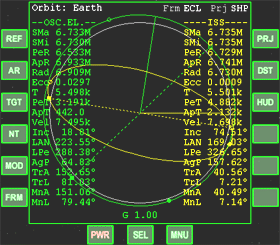
\includegraphics[width=0.5\hsize]{mfd_main.png}
\end{figure}

\noindent
The user interface of an MFD is essentially a computer display (e.g. an LED screen) and a set of input controls (usually push buttons arranged around the screen, or a separate keyboard). In Orbiter, all spacecraft MFDs work the same way, even if the specific layout varies. The picture shows the MFD representation for the generic cockpit view, which supports two MFD positions. 2D panel and virtual cockpit views may use a different number of MFD instruments.\\
In the centre of the MFD is the data display. The 12 buttons along the left and right edge are mode-dependent function buttons. Their labels may change according to the current operation modus of the instrument. The three buttons along the bottom edge are static and perform mode-independent system functions.\\
The MFDs can be operated either by left-clicking the buttons with the mouse, or via the keyboard. All MFD keyboard functions are \Shift-key combinations, where the left and right \Shift keys operate the left and right MFD, respectively. For instrument panels with more than two MFD displays, only two can be operated with the keyboard; the others are limited to mouse control.\\
\\
\textbf{Turning the MFD on and off}\\
The PWR button activates and deactivates the MFD display (keyboard shortcut: \Shift\keystroke{Esc}). In glass cockpit mode, turning off the MFD also hides the buttons (except the power button, so it can be turned on again).\\
\\
\textbf{Mode selection}\\
The SEL button activates the \textit{mode selection screen} (keyboard shortcut: \Ctrl\keystroke{F1}). Each MFD mode provides information for a different navigation or avionics situation (orbital parameters, surface parameters, docking and landing aids, etc.) The default modes are described below in this section. Many additional modes are available via 3$^{rd}$ party add-ons.\\
The mode selection screen shows the available modes in the display area, one mode next to each function button. To select a mode, simply click the corresponding button. For selection with the keyboard, press the \Ctrl key together with the mode selection key displayed in grey with each of the listed modes (for example, \Ctrl\keystroke{O} for Orbit mode).

\begin{figure}[H]
  \centering
  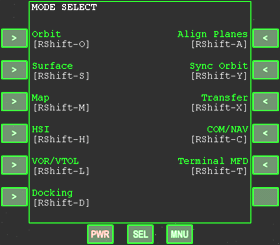
\includegraphics[width=0.5\hsize]{mfd_mode.png}
\end{figure}

\noindent
If there are more modes than can be displayed in a single page, pressing SEL (or \Ctrl\keystroke{F1}) repeatedly cycles through all mode pages. Pressing SEL on the last mode page returns to the previously selected MFD mode. Note that mode selection with keyboard shortcuts works from any of the mode selection pages, even if the requested mode is not displayed on the current page.\\
\\
\textbf{Function buttons}\\
The function of the buttons to the left and right of the display depends on the current MFD mode, and their labels change accordingly. Functions and user interface for the standard MFD modes are described below. For modes provided by 3$^{rd}$ party add-ons, consult the accompanying documentation. In some cases the buttons may act as switches, where each press executes a discrete operation. In other cases it may be necessary to press down a button continuously to adjust a parameter.

\begin{figure}[H]
  \centering
  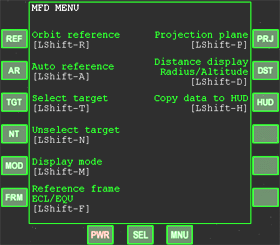
\includegraphics[width=0.5\hsize]{mfd_menu.png}
\end{figure}

\noindent
Function buttons for the two main MFD instruments can also be activated with \Ctrl-key combinations. On pressing the MNU button below the bottom edge of the screen (keyboard shortcut: \Ctrl\keystroke{`}) a short description of all function buttons for this mode is displayed, together with the keyboard shortcuts to activate them. Pressing MNU again, or pressing a function button, restores the display.\\
In glass cockpit view, and in most instrument panels in Orbiter, each MFD has 12 function buttons, but individual spacecraft can adopt a different layout in their panels. If an MFD mode assigns more function buttons than are physically present, pressing MNU repeatedly cycles through the available function pages.\\
\\
\textbf{Colour customisation}\\
The default colour schemes for MFD displays can be modified by editing the Config\textbackslash MFD\textbackslash default.cfg text file. Note that some add-on MFD Modes may define their own colour scheme which cannot be customised.


\subsection{NAV receiver/transmitter setup}
\label{ssec:mfd_comnav}
The \textit{COM/NAV setup} MFD mode provides an interface to the ship's navigation radio receivers which feed data into the navigation instruments. It also allows to select the frequency of the ship's long-range transponder which sends a signal identifying the vessel and its position. The mode is activated via the COM/NAV entry from the MFD mode selection page (shortcut: \Ctrl\keystroke{,} + \Ctrl\keystroke{.}).\\
\\
\textbf{Key options:}

%\begin{table}[H]
	%\centering
	\begin{longtable}{ |p{0.15\textwidth}|p{0.15\textwidth}|p{0.6\textwidth}| }
	\hline\rule{0pt}{2ex}
	\textbf{Button} & \textbf{Shortcut} & \textbf{Action}\\
	\hline\rule{0pt}{2ex}
	SL- & \Shift\keystroke{,} & Move selection up\\
	\hline\rule{0pt}{2ex}
	SL+ & \Shift\keystroke{.} & Move selection down\\
	\hline\rule{0pt}{2ex}
	< & \Shift\keystroke{[} & Step frequency down 0.05 MHz\\
	\hline\rule{0pt}{2ex}
	<{}< & \Shift\keystroke{-} & Step frequency down 1 MHz\\
	\hline\rule{0pt}{2ex}
	> & \Shift\keystroke{]} & Step frequency up 0.05 MHz\\
	\hline\rule{0pt}{2ex}
	>{}> & \Shift\keystroke{=} & Step frequency up 1 MHz\\
	\hline\rule{0pt}{2ex}
	SC< & \Shift\keystroke{Z} & Scan frequency downward\\
	\hline\rule{0pt}{2ex}
	SC> & \Shift\keystroke{X} & Scan frequency upward\\
	\hline
	\end{longtable}
%\end{table}

\noindent
\textbf{MFD control layout:}

\begin{figure}[H]
  \centering
  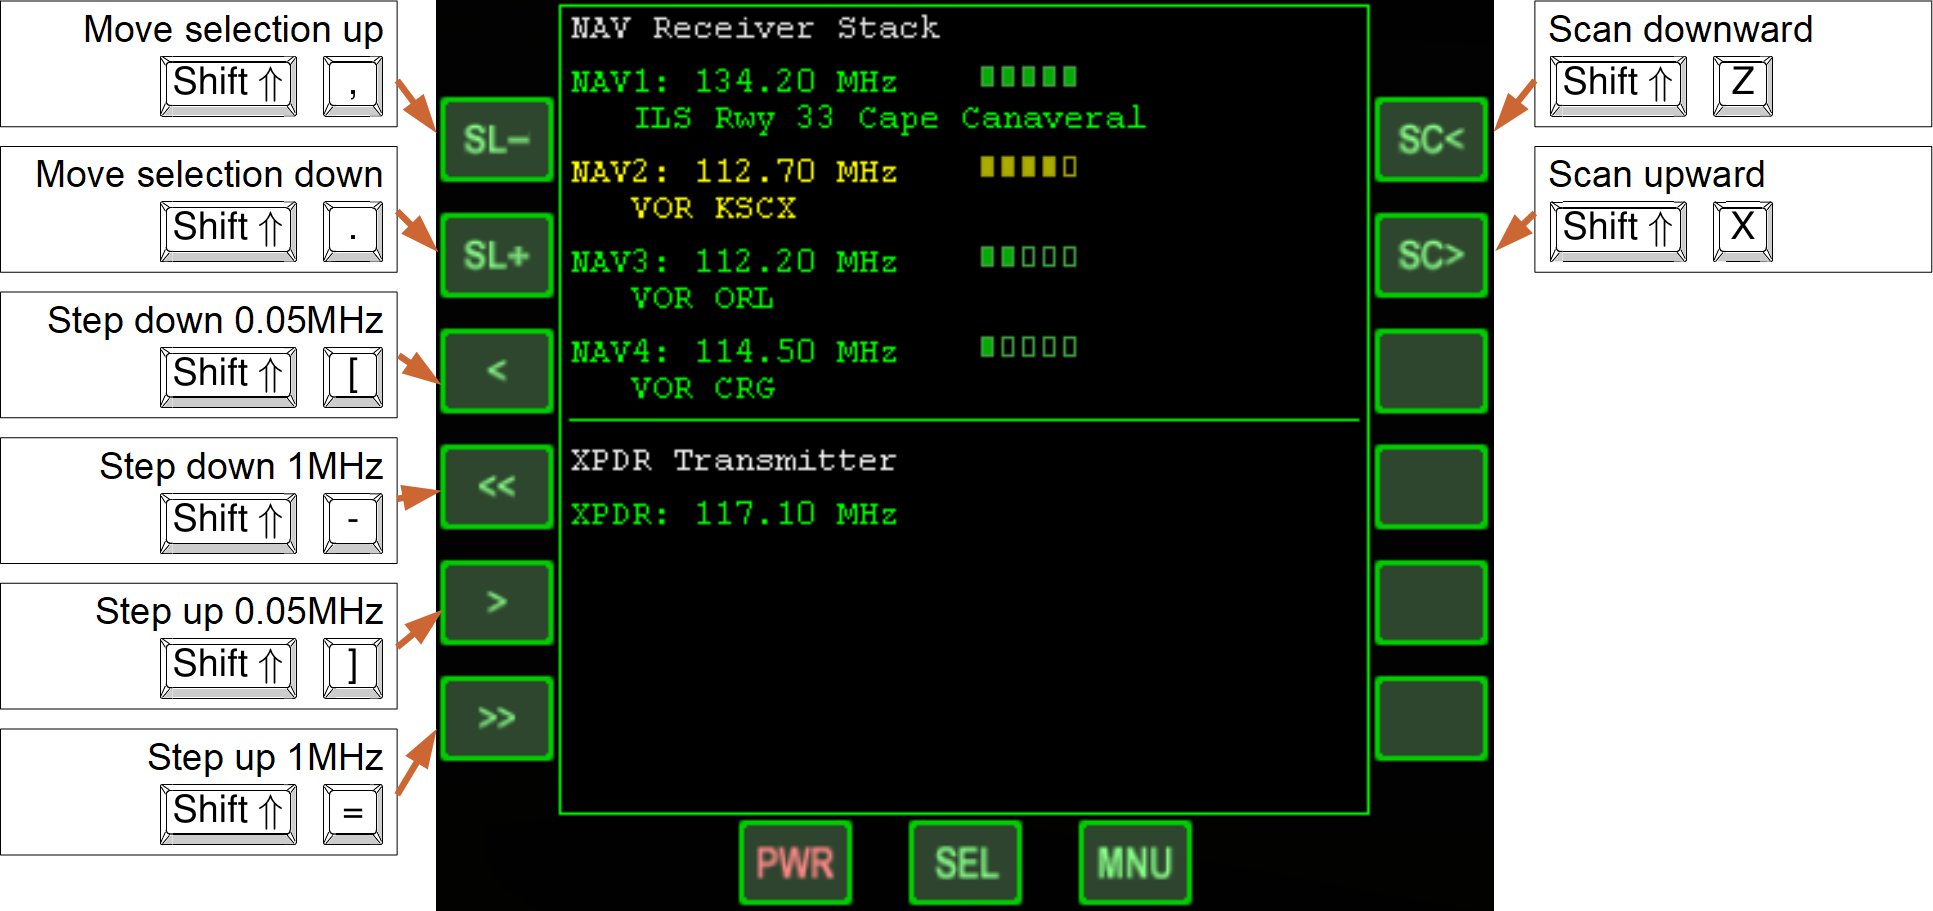
\includegraphics[width=0.99\hsize]{nav_input.png}
\end{figure}

\noindent
\textbf{MFD display components:}\\
The top part of the MFD display shows the NAV radio receiver stack. For each available receiver, the current frequency setting is shown, together with an identification of the received signal (if any) and a field strength indicator. The lower part of the display shows the transponder (XPDR) frequency.\\
The currently selected entry is highlighted in yellow. The selection can be moved up and down with the SL- (or \Shift\keystroke{,}) and SL+ (or \Shift\keystroke{.}) buttons.\\
The frequency of the selected receiver or transmitter can be tuned in steps of 1 MHz with \Shift\keystroke{-} and  \Shift\keystroke{=}, and in steps of 0.05 MHz with \Shift\keystroke{[} and \Shift\keystroke{]}, in the range from 108.00-140.00 MHz. You can sweep the frequency range down or up with \Shift\keystroke{Z} and \Shift\keystroke{X} until a signal is detected. If a compatible NAV transmitter is within range, the instrument displays information about the signal source and strength.

\begin{figure}[H]
  \centering
  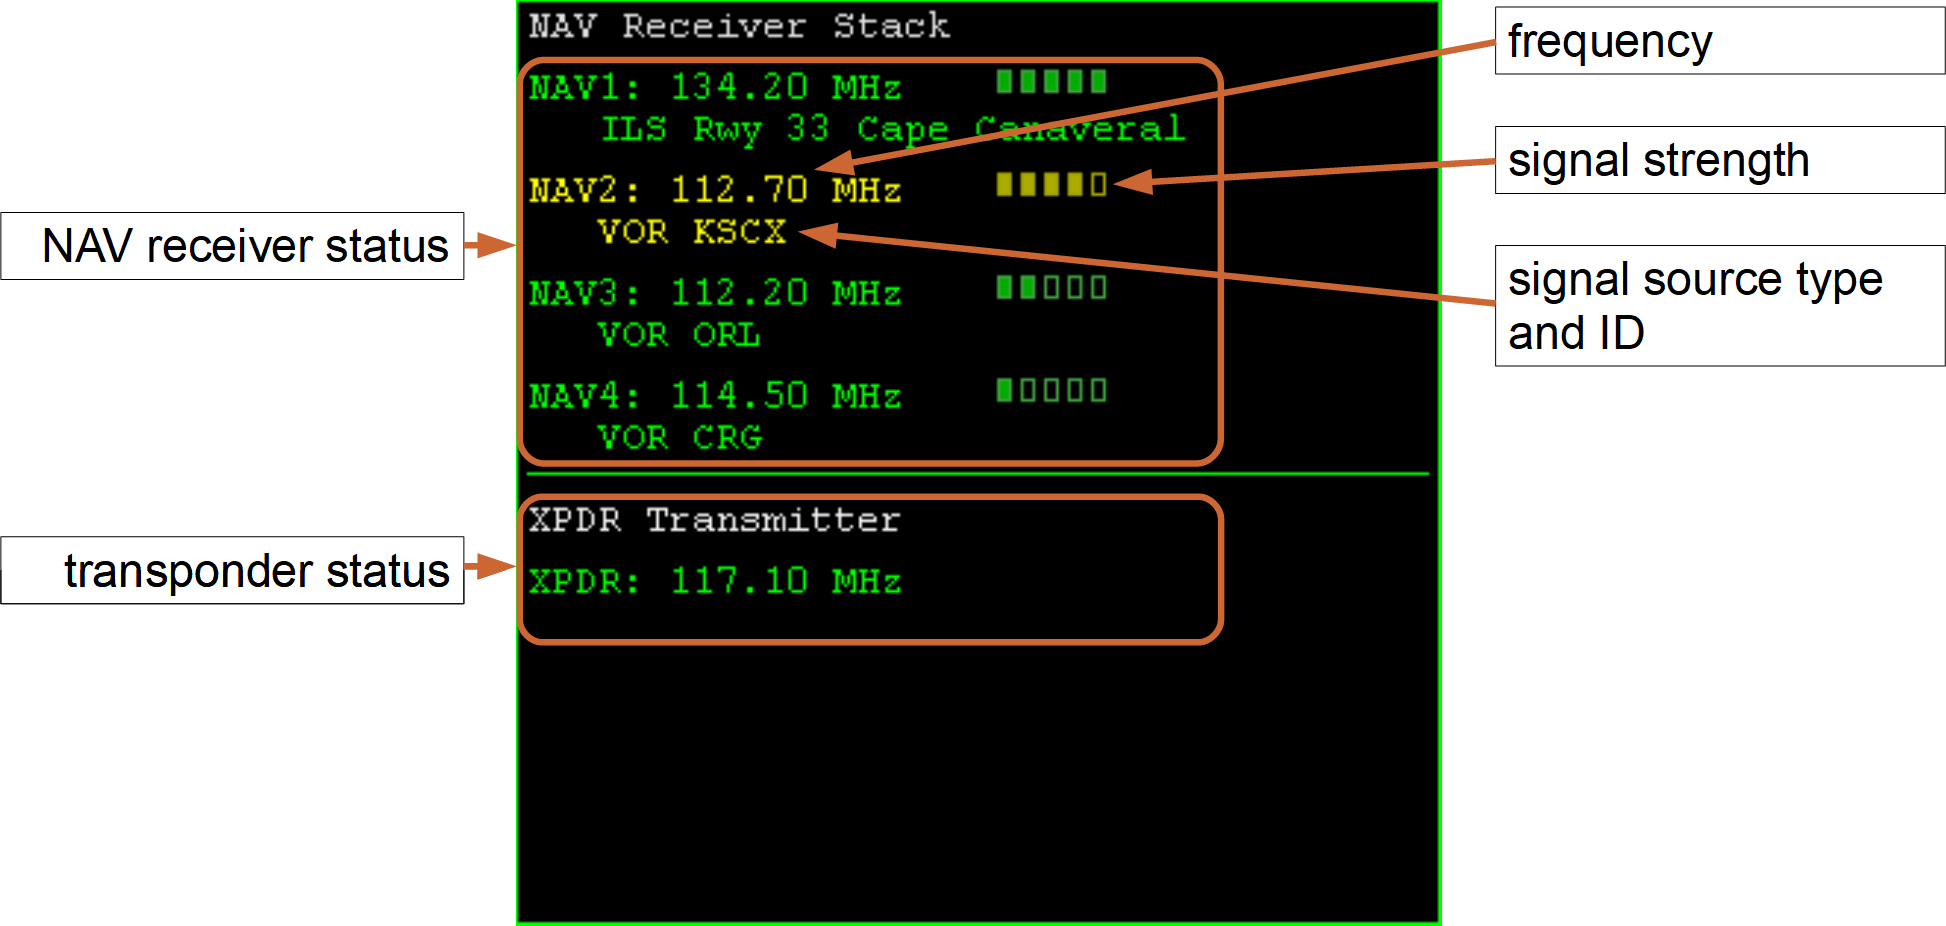
\includegraphics[width=0.99\hsize]{nav_layout.png}
\end{figure}

\noindent
In Orbiter, NAV transmitter types include VOR (VHF omnidirectional range), ILS (instrument landing system) for runway approaches and VTOL (vertical take-off and landing) pads, XPDR (vessel transponders) and IDS (instrument docking system). Each transmitter type provides information which can be fed to other MFD modes or avionics instrumentation to provide situational awareness to the pilot.\\
The \textit{Object info} (\Ctrl\keystroke{I}, see section \ref{ssec:menu_info}) and \textit{Map} (\Ctrl\keystroke{M}, see \ref{ssec:menu_map}) windows are useful tools to obtain surface or vessel-based transmitter frequencies.

\begin{figure}[H]
  \centering
  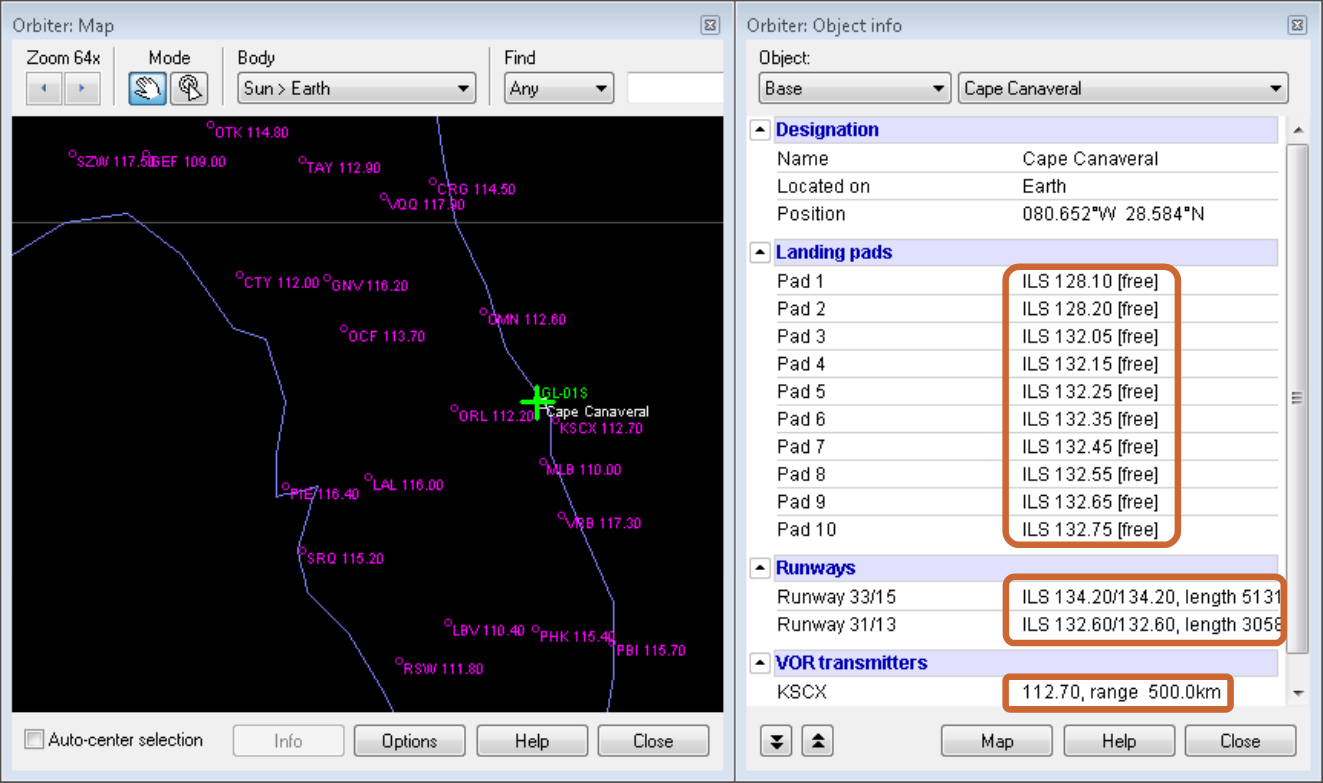
\includegraphics[width=0.75\hsize]{freq_map_info.png}
  \caption{Map window (left) and object info dialog (right) with NAV transmitter information}
\end{figure}

\noindent
The positions and frequencies of VOR stations in your vicinity can also be displayed directly in the simulation window via the VOR Markers option in the \textit{Visual helpers} dialog box (\Ctrl\keystroke{F9}).


\subsection{Surface}
The \textit{Surface} MFD mode provides avionics data useful in flight situations close to planetary surfaces. It contains an attitude indicator (artificial horizon) displaying the vessel's attitude relative to the local horizon plane, various tapes for altitude, speed and acceleration readouts, as well as position, pressure and temperature data.\\
\\
\textbf{Key options:}

%\begin{table}[H]
	%\centering
	\begin{longtable}{ |p{0.15\textwidth}|p{0.15\textwidth}|p{0.6\textwidth}| }
	\hline\rule{0pt}{2ex}
	\textbf{Button} & \textbf{Shortcut} & \textbf{Action}\\
	\hline\rule{0pt}{2ex}
	IAS & \Shift\keystroke{I} & Switch speed readout to indicated airspeed\\
	\hline\rule{0pt}{2ex}
	TAS & \Shift\keystroke{T} & Switch speed readout to true airspeed\\
	\hline\rule{0pt}{2ex}
	GS & \Shift\keystroke{G} & Switch speed readout to ground-relative speed\\
	\hline\rule{0pt}{2ex}
	OS & \Shift\keystroke{O} & Switch speed readout to orbital speed\\
	\hline\rule{0pt}{2ex}
	HUD & \Shift\keystroke{H} & Set HUD to Surface mode\\
	\hline
	\end{longtable}
%\end{table}

\noindent
\textbf{MFD control layout:}

\begin{figure}[H]
  \centering
  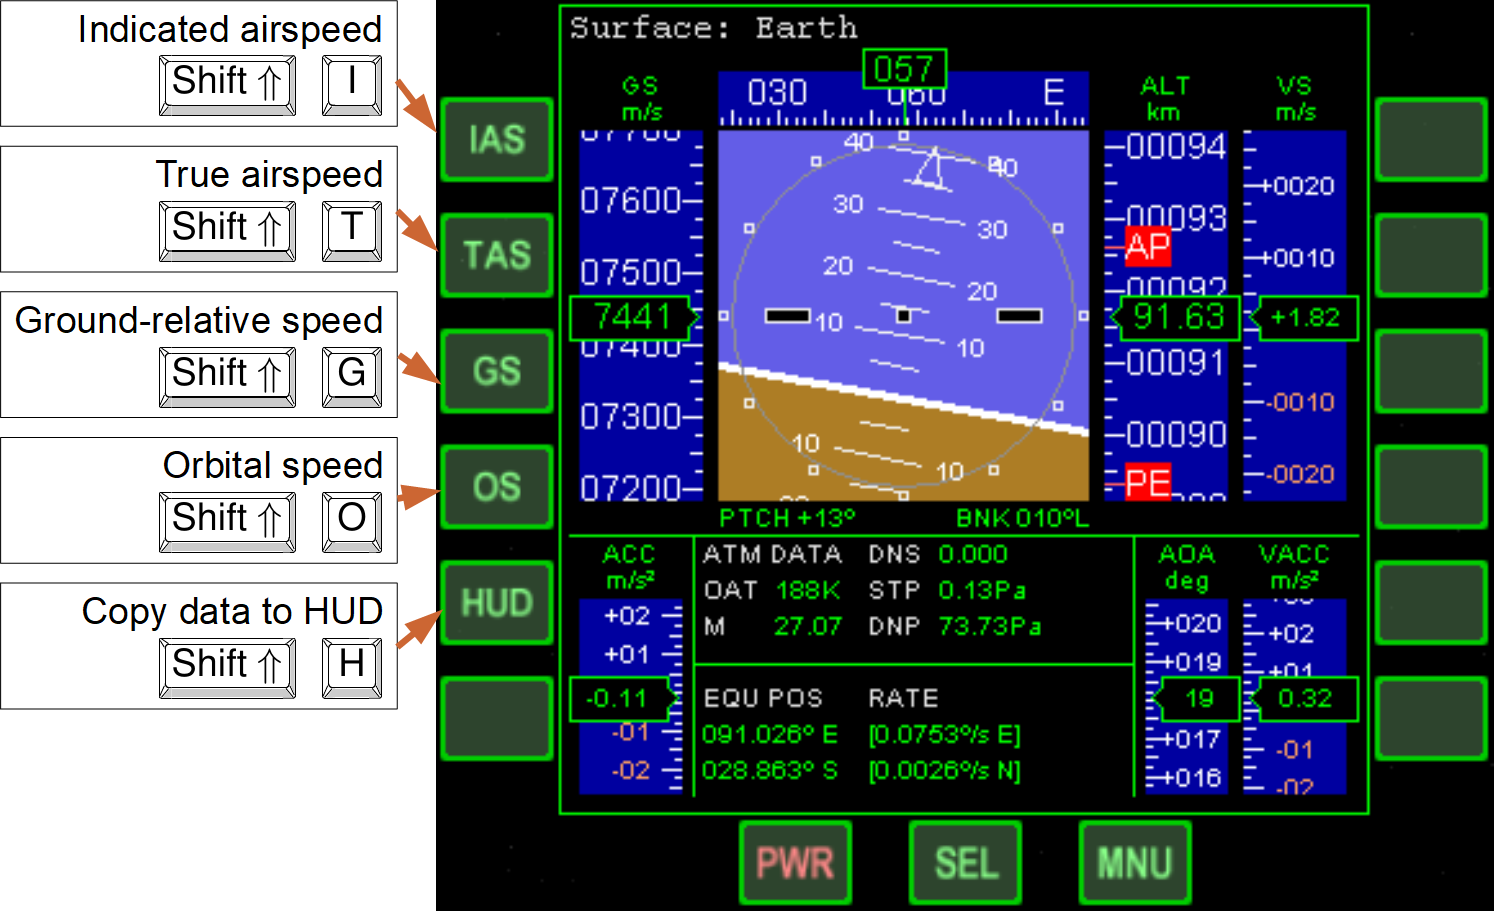
\includegraphics[width=0.75\hsize]{surface_input.png}
\end{figure}

\noindent
\textbf{MFD display components:}\\
The display contains an attitude indicator (AI) with horizon line and pitch ladder indicating pitch and bank attitude (including numerical readouts). Above is a compass ribbon with a heading readout. To the left of the AI is the speed readout which can be set to different modes with the MFD buttons:

\begin{itemize}
\item TAS (true airspeed): The speed of the spacecraft relative to the surrounding atmosphere. Airspeed is usually measured with a pitot tube in the airstream recording the difference between free-stream and stagnation point pressure. The TAS mode is only available if the free-stream pressure $p_{1}$ > 10$^{-3}$ Pa (on Earth, this corresponds to approx. 140 km altitude). If TAS cannot be measured, the speed tape is reset to 0 and the readout shows "-{}-{}-{}-".
\item IAS (indicated airspeed): Commonly used in conventional aircraft. IAS is calibrated to atmospheric density and speed of sound at sea level. IAS and TAS are similar at low altitude, but start to diverge at higher altitudes, with IAS < TAS. The limit $p_{1}$ > 10$^{-3}$ Pa also applies to IAS availability.
\item GS (ground-relative speed): The magnitude of the vessel's velocity vector in the rotating planet reference frame. This is similar to TAS at lower altitudes, but diverges at higher altitudes. Usually, TAS is no longer available where the differences would become significant. \textit{Note:} for an object in geostationary orbit, GS would be zero since it is stationary relative to the rotating planet frame.
\item OS (orbital speed): The magnitude of the vessel's velocity relative to the planet's centre in a non-rotating frame. This is identical to the Vel readout in the \textit{Orbit} MFD. Note: OS is usually non-zero for a vessel at rest on the planet surface, because the planet itself is rotating.
\end{itemize}

\begin{figure}[H]
  \centering
  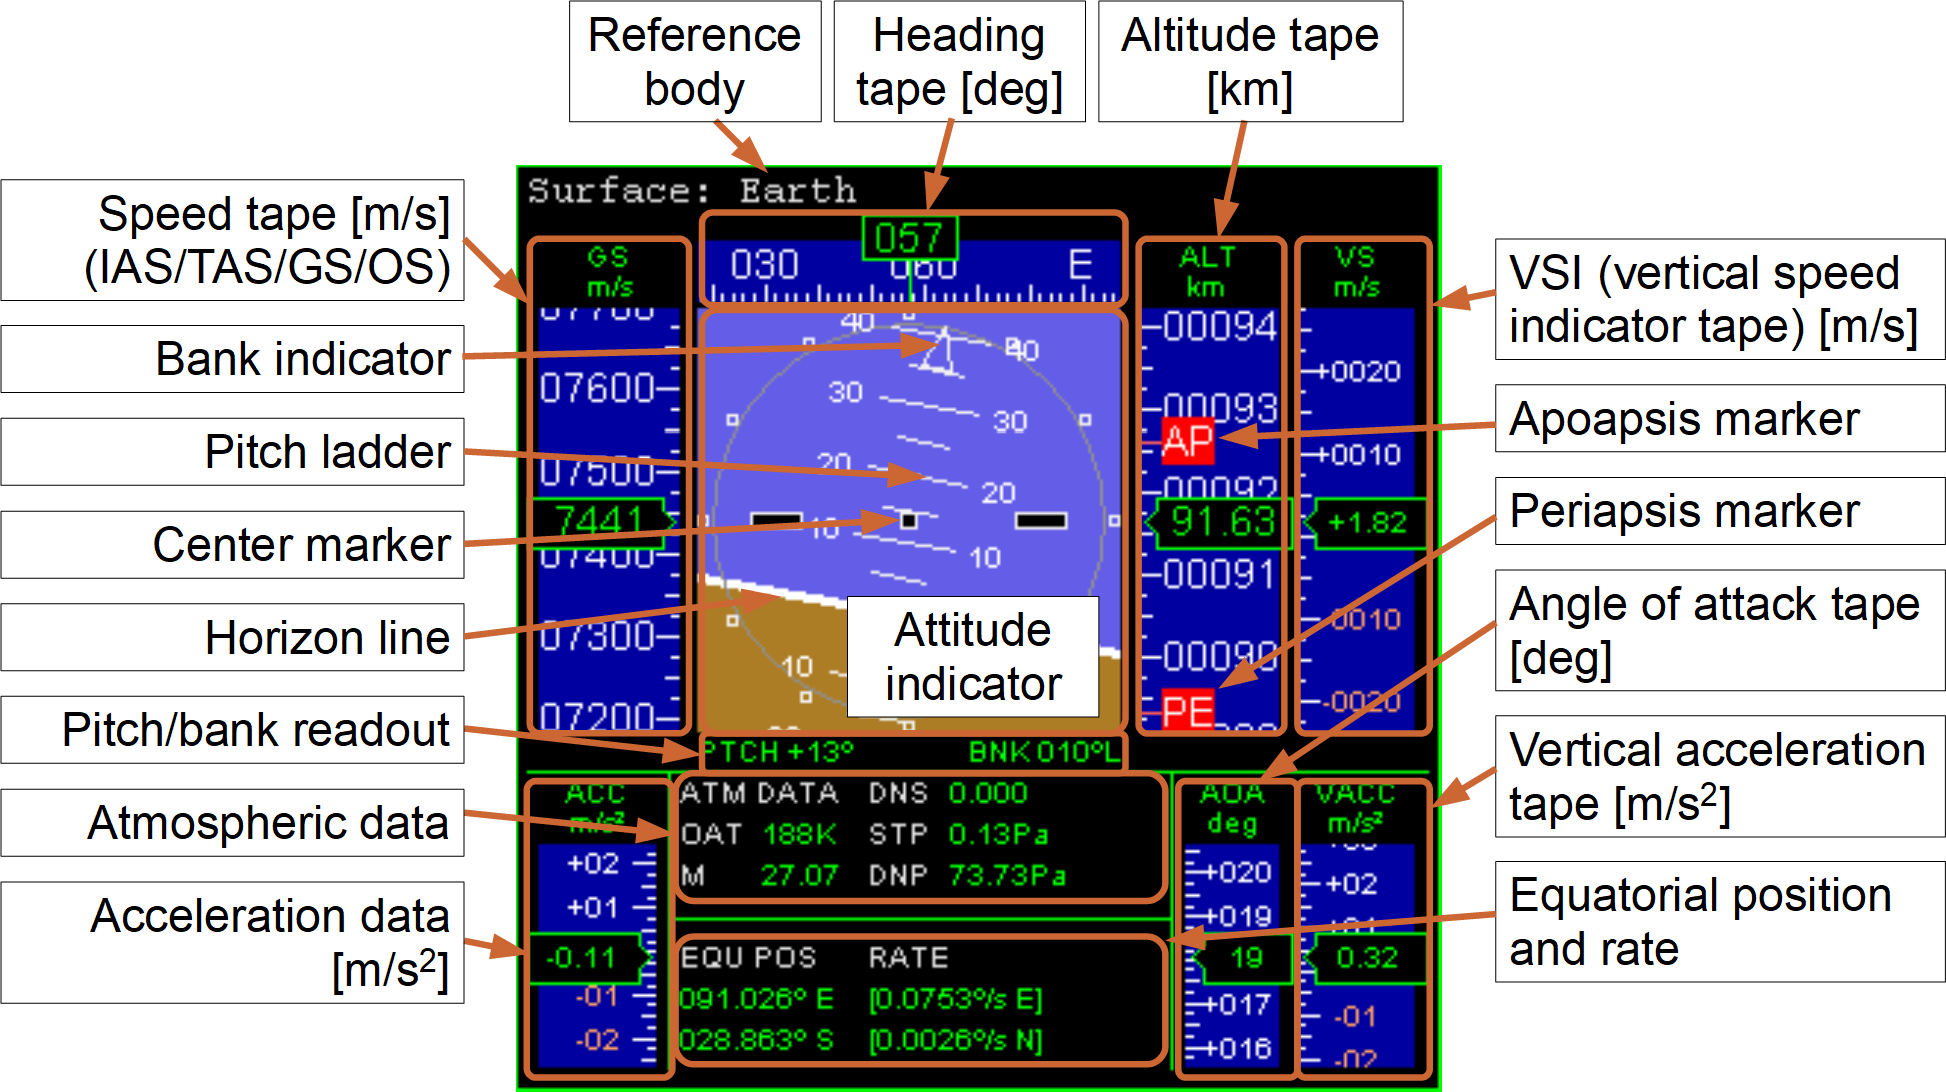
\includegraphics[width=0.99\hsize]{surface_layout.png}
\end{figure}

\noindent
To the right of the IA is the altitude tape showing the vessel altitude [km] above the surface (ALT-R) at altitudes < 10 km, or altitude above mean planet radius (ALT) otherwise. To the right of the altitude tape is the vertical speed tape (VS) [m/s].\\
In the lower part of the display are the acceleration tape (ACC) [m/s$^{2}$] (left), and the AOA (angle of attack) and vertical acceleration (VACC) [m/s$^{2}$] tapes (right).\\
Below the AI are atmospheric data readouts: atmospheric density (DNS), static pressure (STP), dynamic pressure (DNP), outside air temperature (OAT) and Mach number (M). In the block below are vessel's equatorial position (longitude, latitude) [deg] and their rates [deg/s].


\subsection{Map}
\label{ssec:mfd_map}
The \textit{Map} MFD mode shows the surface of a celestial body in a cylindrical projection, including coastlines and contour lines. It can display surface markers for bases and VOR beacons, as well as ground tracks or orbital plane intersections for objects orbiting the body. The display elements are similar to the \textit{Map} dialog (see section \ref{ssec:menu_map}).\\
\\
\textbf{Key options (map view):}

%\begin{table}[H]
	%\centering
	\begin{longtable}{ |p{0.15\textwidth}|p{0.15\textwidth}|p{0.6\textwidth}| }
	\hline\rule{0pt}{2ex}
	\textbf{Button} & \textbf{Shortcut} & \textbf{Action}\\
	\hline
	\multicolumn{3}{|c|}{\rule{0pt}{2ex}\textbf{\textit{Map view:}}}\\
	\hline\rule{0pt}{2ex}
	REF & \Shift\keystroke{R} & Select a celestial body for map display\\
	\hline\rule{0pt}{2ex}
	TGT & \Shift\keystroke{T} & Select a target object\\
	\hline\rule{0pt}{2ex}
	ZM- & \Shift\keystroke{X} & Zoom out by factor 2 down to 1x (global view)\\
	\hline\rule{0pt}{2ex}
	ZM+ & \Shift\keystroke{Z} & Zoom in by factor 2 up to 128x (2.8° x 2.8° cover)\\
	\hline\rule{0pt}{2ex}
	TRK & \Shift\keystroke{K} & Toggle automatic vessel track mode on/off\\
	\hline\rule{0pt}{2ex}
	DSP & \Shift\keystroke{D} & Display parameter configuration page\\
	\hline\rule{0pt}{2ex}
	UP & \Shift\keystroke{-} & Scroll map display up (disabled in track mode)\\
	\hline\rule{0pt}{2ex}
	DN & \Shift\keystroke{=} & Scroll map display down (disabled in track mode)\\
	\hline\rule{0pt}{2ex}
	< & \Shift\keystroke{[} & Scroll map display left (disabled in track mode)\\
	\hline\rule{0pt}{2ex}
	> & \Shift\keystroke{]} & Scroll map display right (disabled in track mode)\\
	\hline
	\multicolumn{3}{|c|}{\rule{0pt}{2ex}\textbf{\textit{Parameter selection view:}}}\\
	\hline\rule{0pt}{2ex}
	UP & \Shift\keystroke{-} & Move selection marker up\\
	\hline\rule{0pt}{2ex}
	DN & \Shift\keystroke{=} & Move selection marker down\\
	\hline\rule{0pt}{2ex}
	MOD & \Shift\keystroke{M} & Modify the currently selected option\\
	\hline\rule{0pt}{2ex}
	OK & \Shift\keystroke{O} & Return to map view\\
	\hline
	\end{longtable}
%\end{table}

\noindent
\textbf{MFD control layout:}

\begin{figure}[H]
  \centering
  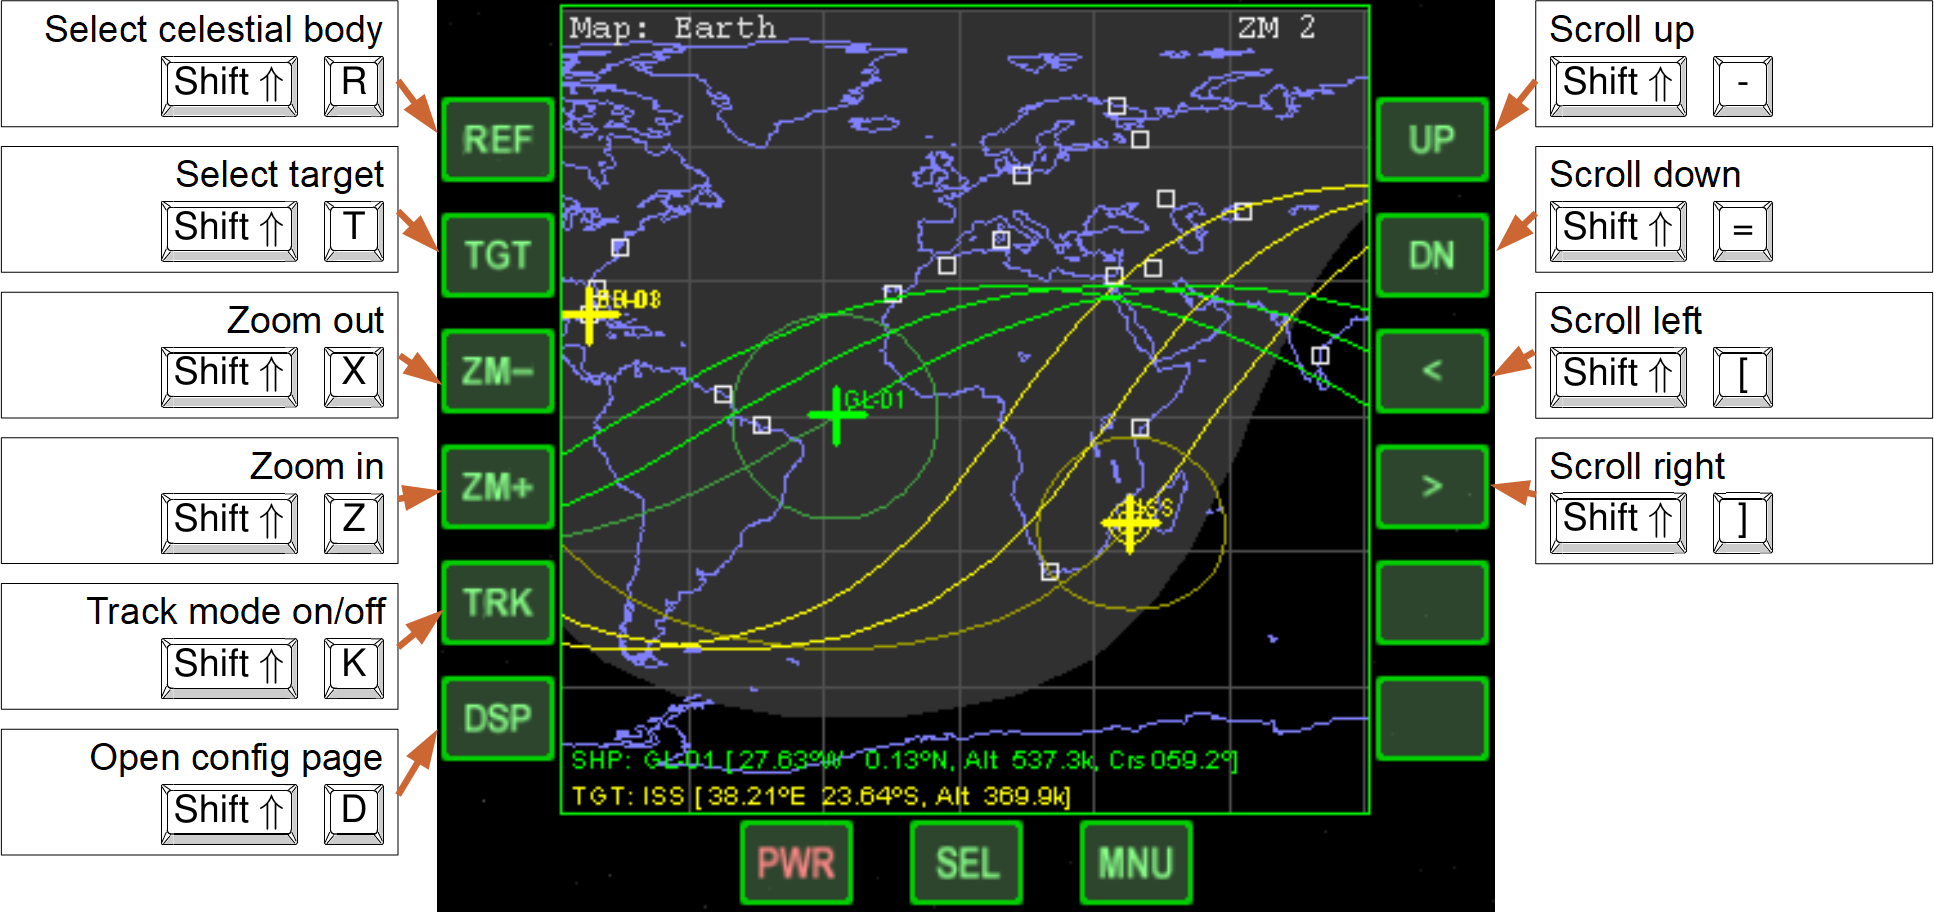
\includegraphics[width=0.99\hsize]{map_input.png}
\end{figure}

\noindent
\textbf{MFD display components:}\\
The map display elements include:

\begin{itemize}
\item Current position (green +) projected onto the planet surface.
\item Positions of any other spacecraft currently located on the planet surface or orbiting the planet (yellow +)
\item Orbit ground track (past and predicted for a few orbits), or alternatively orbit plane (the great circle defined by the intersection of the orbital plane with the planet surface)
\item Horizon line: indicates the limit of visibility of the planet surface as seen from the current vessel position (or equivalently, the area of the planet surface from which the spacecraft would appear above the horizon for a ground-based observer).
\item Terminator line: indicates the lit hemisphere of the planet with a boundary line and/or a shaded area.
\item Coastlines and contour lines (e.g. topographical levels) where supported.
\item Location of surface bases, VOR transmitters with frequencies and other surface features (cities or geological features)
\item The current position (longitude, latitude, altitude) and course of the vessel, and the position data of an optional target object or surface base are shown at the bottom of the screen. If the target is a base, distance and bearing from the current vessel position are also displayed.
\end{itemize}

\noindent
The map can be zoomed and scrolled. It is also possible track the current position (which disables manual scrolling). At high zoom levels, labels for marked surface features are shown.

\begin{figure}[H]
  \centering
  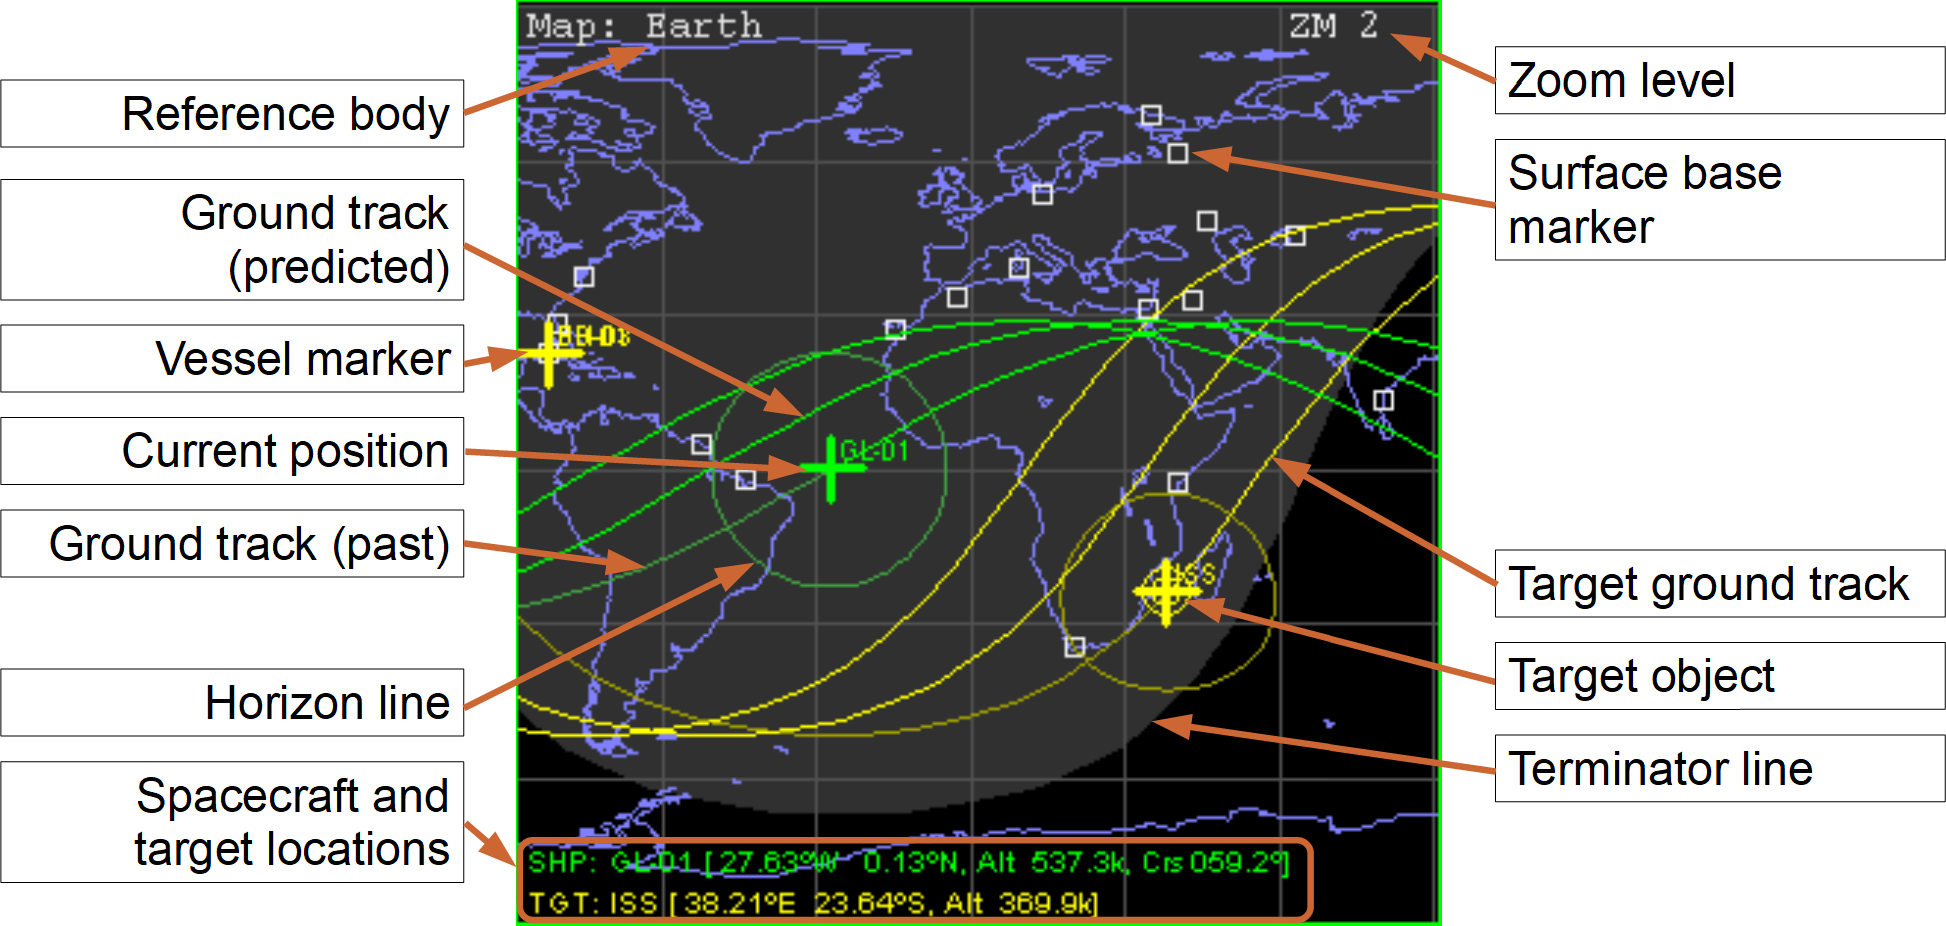
\includegraphics[width=0.99\hsize]{map_layout_1.png}
\end{figure}

\begin{figure}[H]
  \centering
  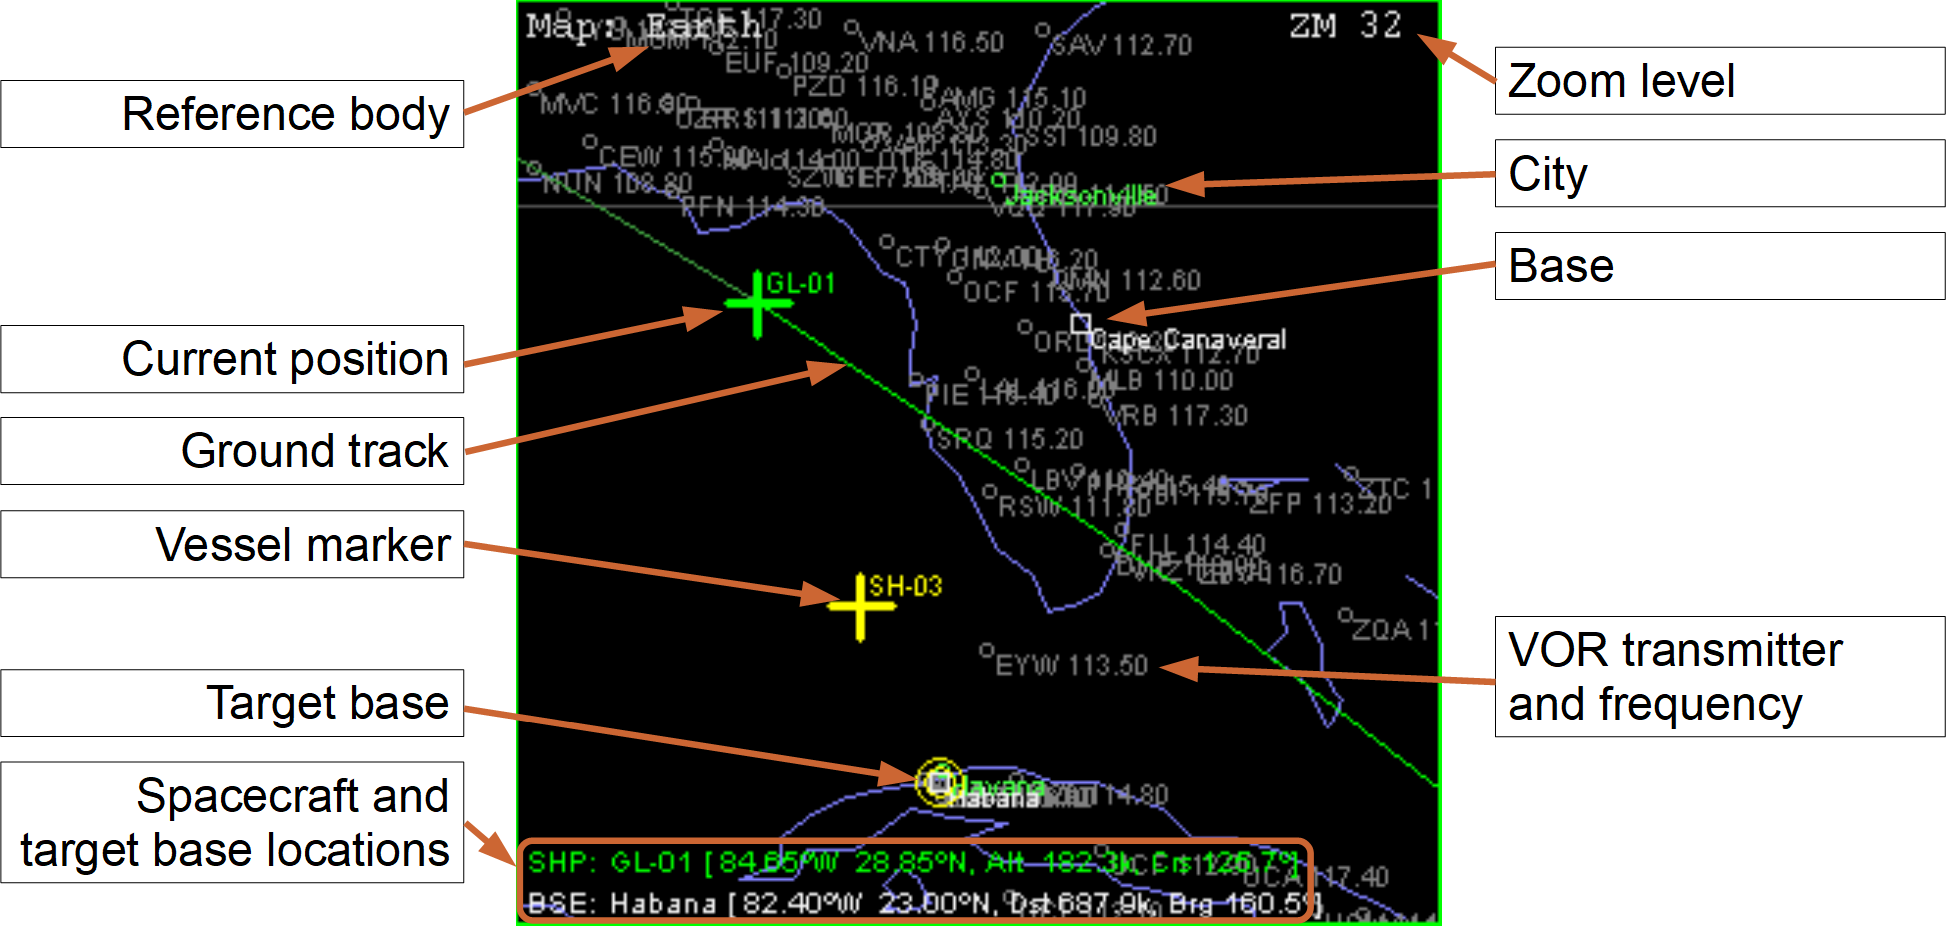
\includegraphics[width=0.99\hsize]{map_layout_2.png}
\end{figure}

\noindent
Display options can be selected from the configuration page (DSP, \Shift\keystroke{D}). Select an item with the UP (\Shift\keystroke{-}) and DN (\Shift\keystroke{=}) buttons, then cycle its settings with MOD (\Shift\keystroke{M}). Return to the map screen with OK (\Shift\keystroke{O}).

\begin{figure}[H]
  \centering
  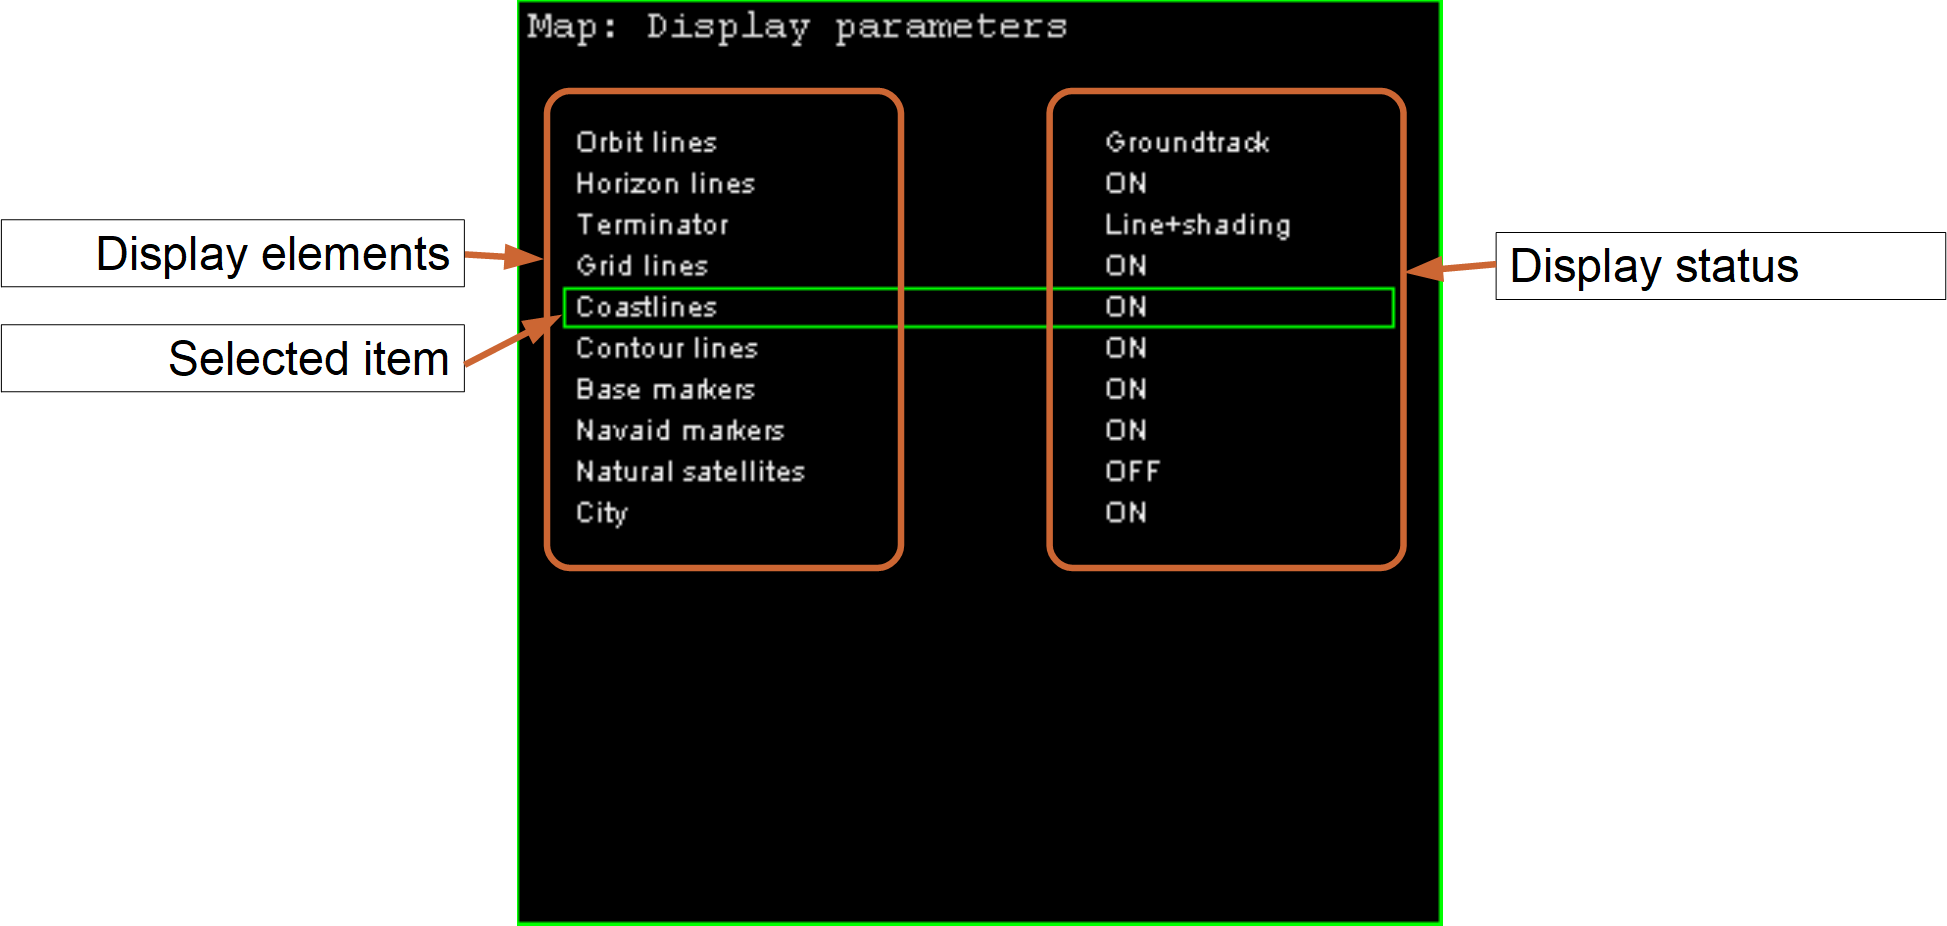
\includegraphics[width=0.99\hsize]{map_params.png}
\end{figure}

\begin{itemize}
\item Only objects (ships, stations or moons) orbiting the displayed celestial body will be accepted as orbit targets. Likewise, only surface bases located on the body will be accepted as target bases.
\item Your ship's orbital plane will only be plotted if you are orbiting the displayed body.
\end{itemize}


\subsection{VOR/VTOL}
The VOR/VTOL MFD mode is a navigational aid that provides position information with respect to a signal transmitter (VOR) or a landing pad for vertical take-off and landing. (see also section \ref{ssec:mfd_hsi} on HSI mode). The circular display on the left shows a top-down view of the transmitter location and bearing relative to the current vessel position in the centre of the display. The two bars to the right show vessel altitude and vertical speed.\\
This MFD mode can be linked to one of the ship's NAV receivers. The current receiver and frequency are shown in the upper right corner of the display. If a signal is received, the transmitter ID is displayed in the second line. If the ship is equipped with more than a single NAV receiver, the receiver stack can be cycled with \Shift\keystroke{N}. To set the receiver frequencies, use the COM/NAV MFD mode (see section \ref{ssec:mfd_comnav}).\\
\\
\textbf{Key options:}

%\begin{table}[H]
	%\centering
	\begin{longtable}{ |p{0.15\textwidth}|p{0.15\textwidth}|p{0.6\textwidth}| }
	\hline\rule{0pt}{2ex}
	\textbf{Button} & \textbf{Shortcut} & \textbf{Action}\\
	\hline\rule{0pt}{2ex}
	NAV & \Shift\keystroke{N} & Select navigation (NAV) receiver for VOR or VTOL information input.\\
	\hline
	\end{longtable}
%\end{table}

\noindent
\textbf{MFD control layout:}

\begin{figure}[H]
  \centering
  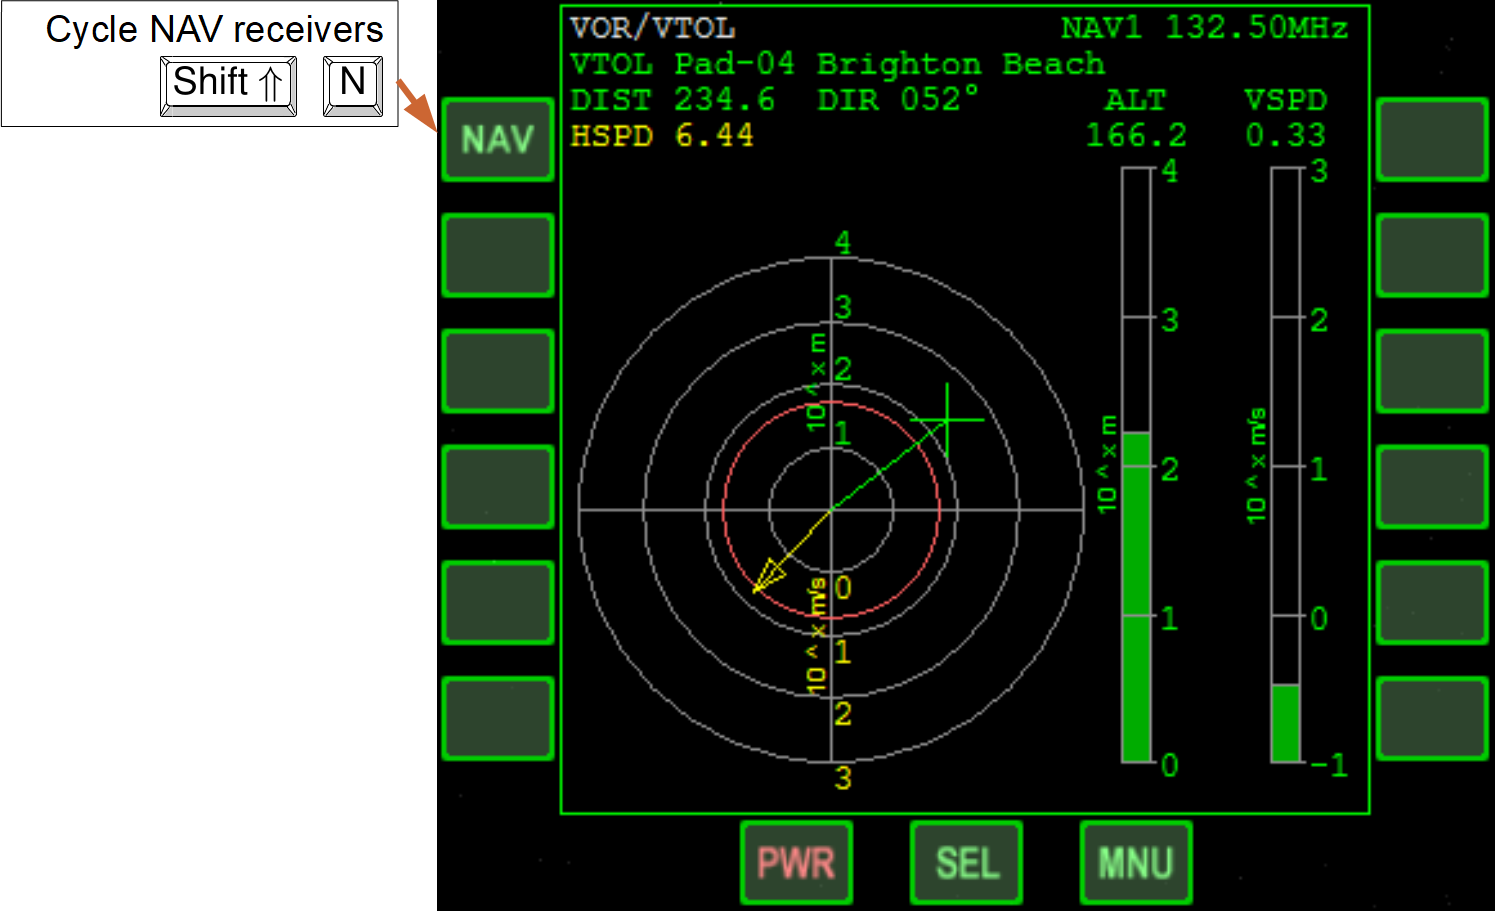
\includegraphics[width=0.75\hsize]{vorvtol_input.png}
\end{figure}

\noindent
\textbf{MFD display components:}

\begin{figure}[H]
  \centering
  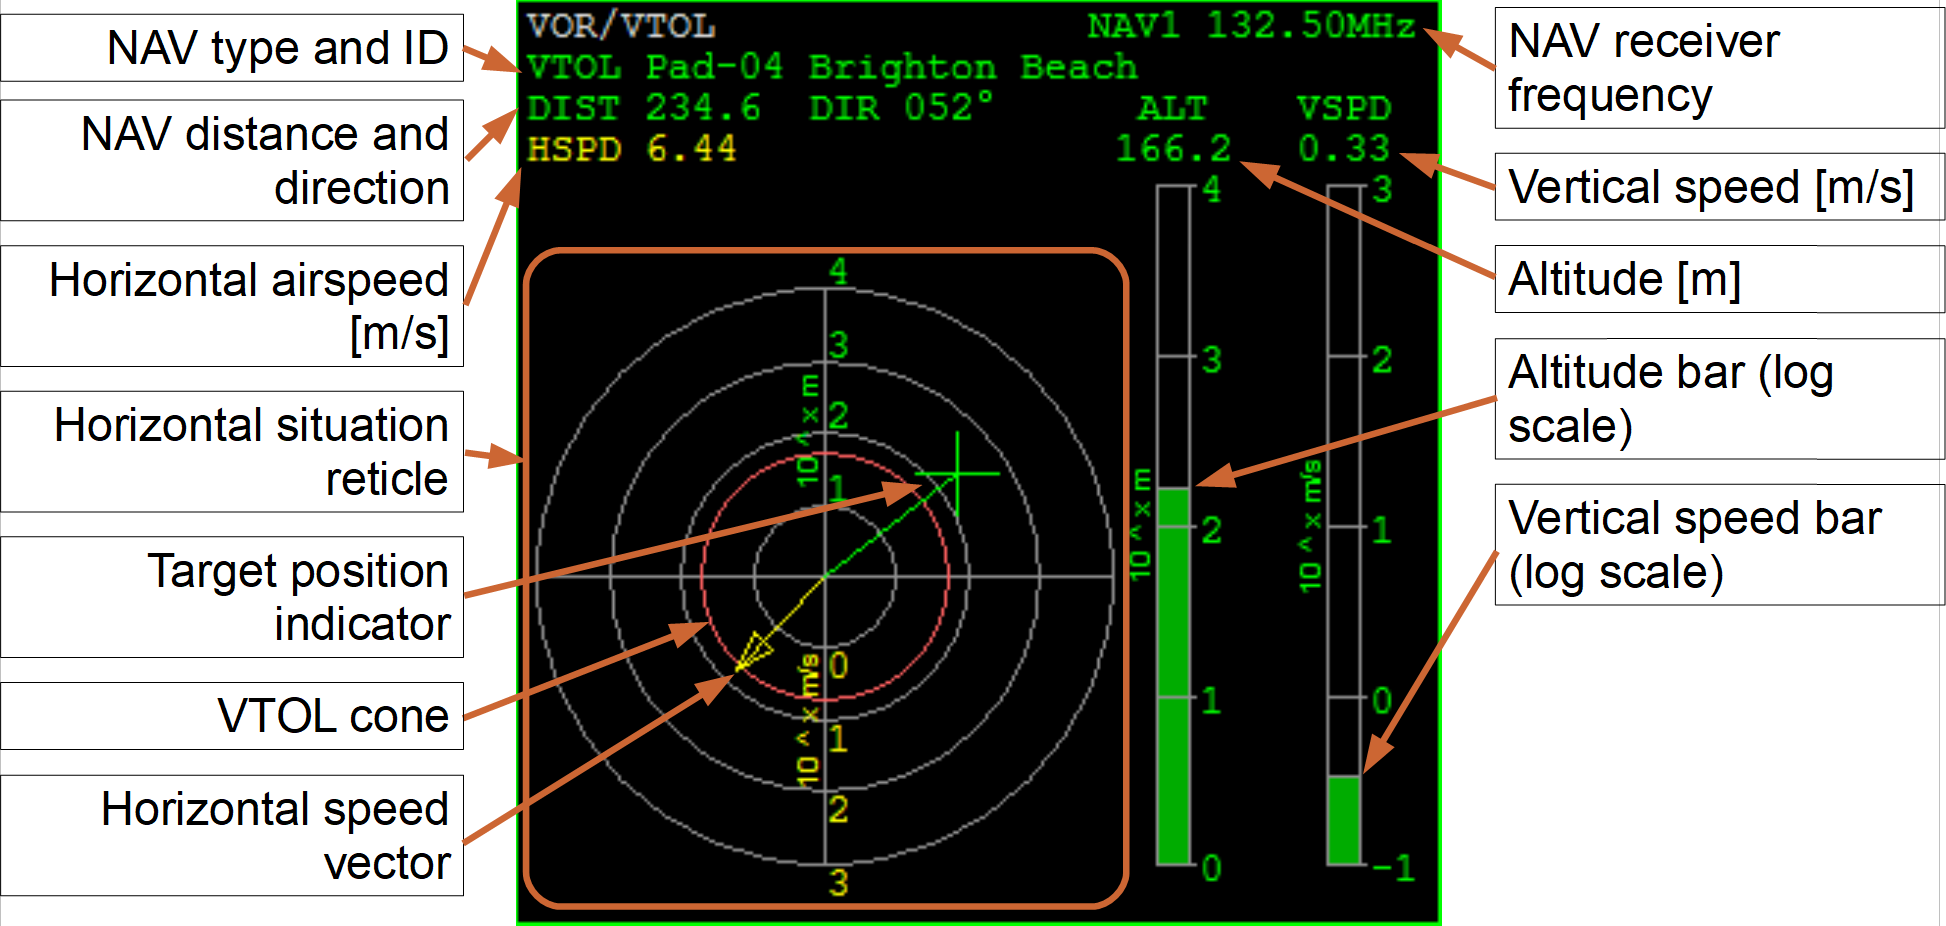
\includegraphics[width=0.99\hsize]{vorvtol_layout.png}
\end{figure}

\begin{itemize}
\item \textbf{DIST:} distance to NAV transmitter [m]
\item \textbf{DIR:} NAV transmitter direction (ship-relative)
\item \textbf{HSPD:} horizontal airspeed [m/s]
\item \textbf{ALT:} altitude [m]. The altitude bar has a range from 1 to 10$^{4}$ m (logarithmic scale)
\item \textbf{VSPD:} vertical airspeed [m/s]. The vertical speed bar has a range from $\pm$0.1 to $\pm$10$^{3}$ m/s (logarithmic scale). Positive vertical speed is indicated by a green bar, negative vertical speed by a yellow or red bar. \textit{Red} is a surface impact warning.
\item \textbf{Horizontal reticle:} Top-down view with the vessel in the centre pointing towards the 12 o'clock position. 
\item \textbf{Target indicator:} Shows the horizontal location of the transmitter source (green cross) relative to the vessel. The radial scale is logarithmic with a range from 1 to 10$^{4}$ m.
\item \textbf{Hspeed vector:} Yellow arrow shows the horizontal component of the speed vector (vessel-relative). The radial scale is logarithmic with a range from 0.1 to 10$^{3}$ m/s.
\item \textbf{VTOL cone:} This circle indicates the admissible horizontal displacement from the landing pad centre during descent for vertical landing. The circle becomes smaller with decreasing altitude. The target position marker should be kept inside the cone during descent. A red circle signals too large a displacement. The VTOL cone is displayed only if the MFD is linked to a VTOL transmitter signal.
\end{itemize}


\subsection{Horizontal Situation Indicator}
\label{ssec:mfd_hsi}
The Horizontal Situation Indicator (HSI) consists of two independent displays. Each display can be linked to a NAV receiver and show directional and relative bearing information from surface-based transmitters such as VOR (very high frequency omnidirectional range) and ILS (instrument landing system). The operation of the displays is similar to instrument navigation systems found in aircraft.\\
Each display represents a gyro-compass indicating the current heading at the 12 o'clock position. The yellow arrow in the centre of the display is the \textit{course arrow} or \textit{Omni Bearing Selector} (OBS). When the linked NAV receiver is tuned to a VOR transmitter, the OBS can be adjusted with the OB- (\Shift\keystroke{[}) and OB+ (\Shift\keystroke{]}) keys. For ILS transmitters, the OBS is automatically fixed to the approach direction.\\
The middle section of the course arrow is the \textit{Course Deviation Indicator} (CDI). It can deflect to the left and right to show the deviation of the OBS setting from the current bearing to the NAV transmitter. If the CDI is deflected to the left, then the selected radial is to the left of the current position.\\
In the lower left corner of the display is the TO/FROM indicator. "TO" means that you are working with a bearing from you \textit{to} the ground station. "FROM" indicates a radial \textit{from} the ground station to you.\\
When tuned to an ILS (instrument landing system) transmitter, the display shows an additional horizontal glide-slope bar for vertical guidance to the runway. If the bar is centred in the instrument, you are on the correct glide-slope. If it is above the centreline, the glide-slope is \textit{above} you, i.e. you are too low. If it is below the centreline, the glide-slope is \textit{below} you and you are approaching too high. For instrument-guided landing approaches see also section \ref{ssec:basic_landing}.\\
The refresh rate for the HSI MFD mode is 4 Hz or the user selection in the Launchpad dialog, whichever is higher.\\
\\
\textbf{Key options:}

%\begin{table}[H]
	%\centering
	\begin{longtable}{ |p{0.15\textwidth}|p{0.15\textwidth}|p{0.6\textwidth}| }
	\hline\rule{0pt}{2ex}
	\textbf{Button} & \textbf{Shortcut} & \textbf{Action}\\
	\hline\rule{0pt}{2ex}
	L/R & \Shift\keystroke{F} & Switch focus between left/right HSI display\\
	\hline\rule{0pt}{2ex}
	NAV & \Shift\keystroke{N} & Cycle through NAV receiver stack\\
	\hline\rule{0pt}{2ex}
	OB- & \Shift\keystroke{[} & Rotate OBS left\\
	\hline\rule{0pt}{2ex}
	OB+ & \Shift\keystroke{]} & Rotate OBS right\\
	\hline
	\end{longtable}
%\end{table}

\noindent
\textbf{MFD control layout:}

\begin{figure}[H]
  \centering
  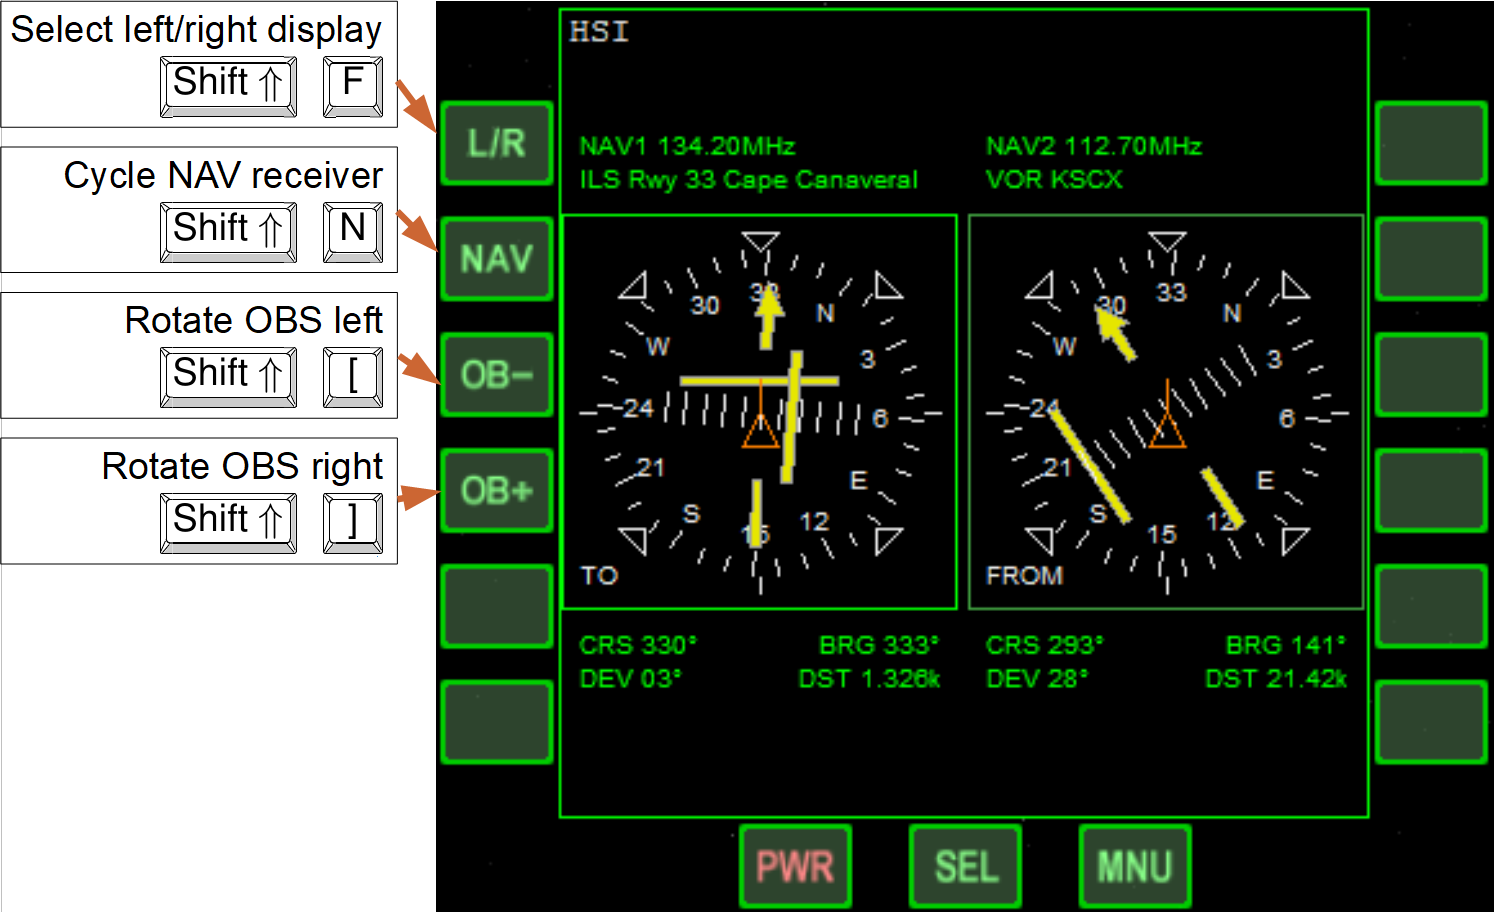
\includegraphics[width=0.75\hsize]{hsi_input.png}
\end{figure}

\noindent
\textbf{MFD display components:}

\begin{figure}[H]
  \centering
  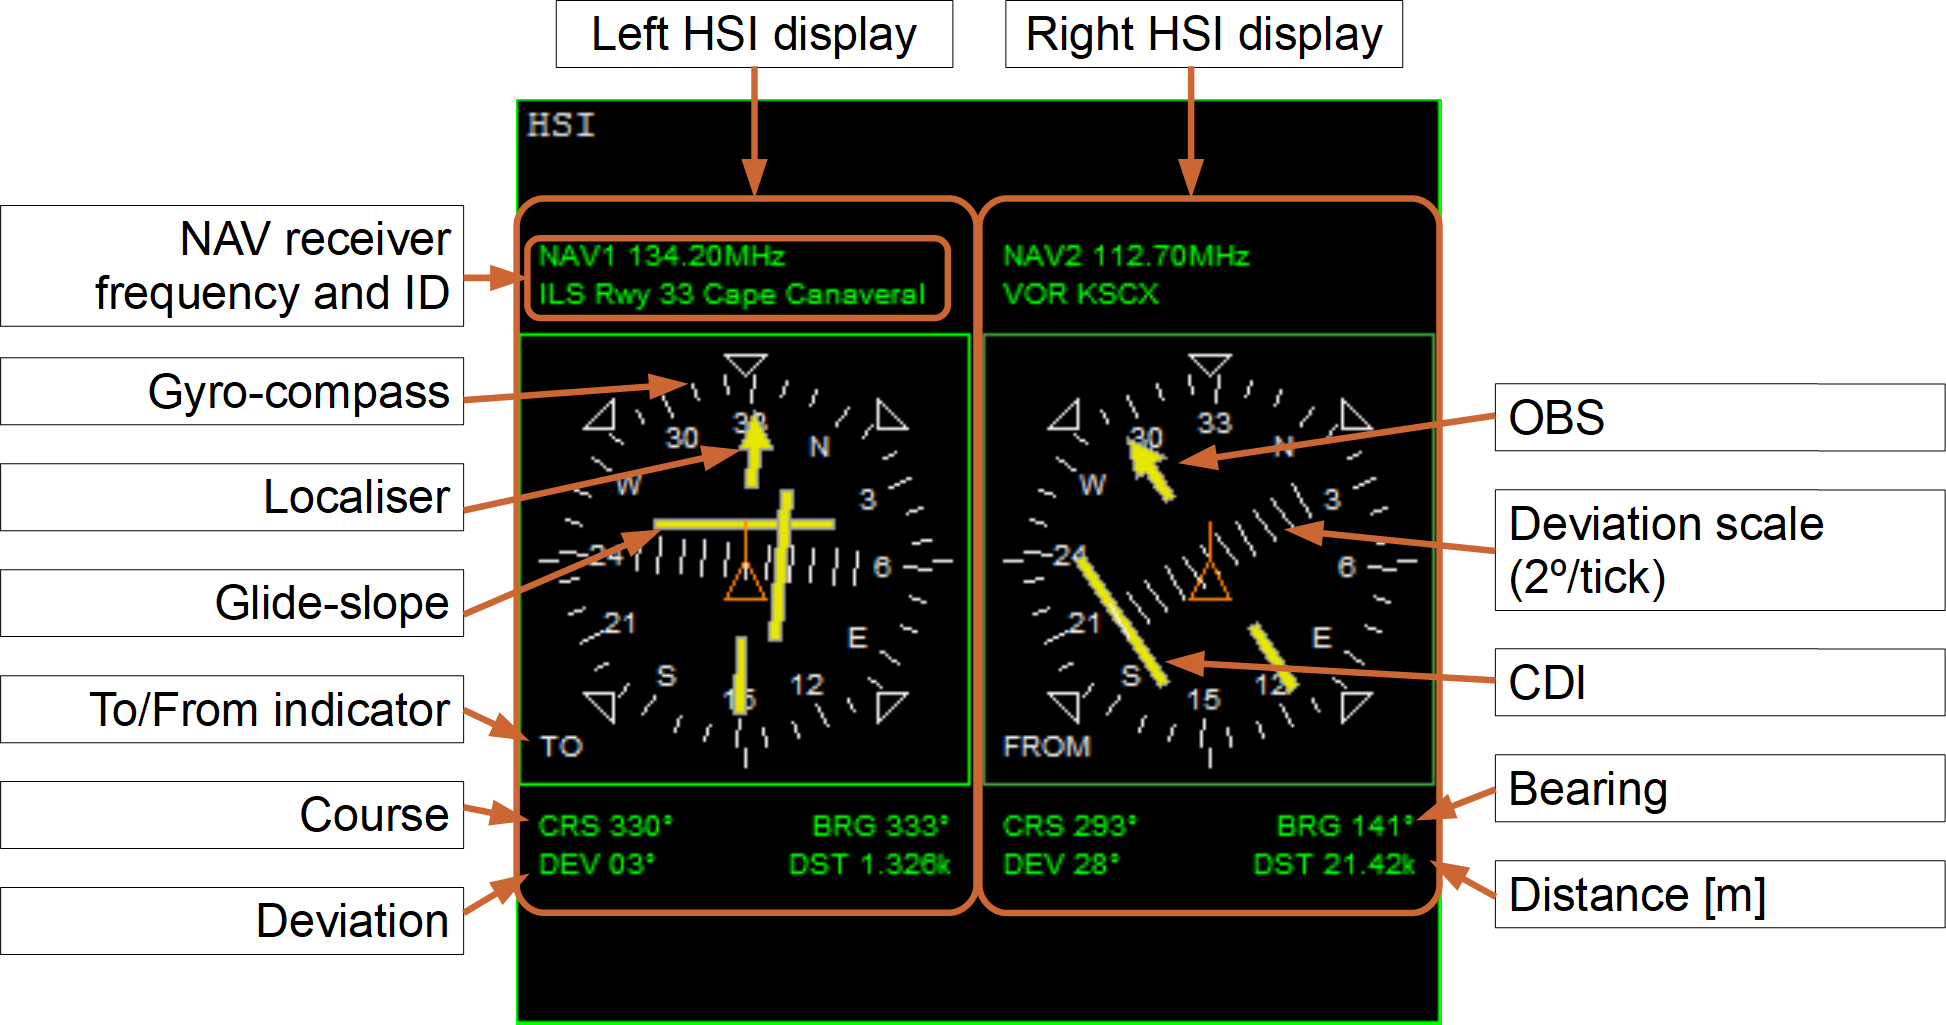
\includegraphics[width=0.99\hsize]{hsi_layout.png}
\end{figure}

\noindent
\textbf{To use the HSI for surface navigation:}

\begin{itemize}
\item Determine the frequency of the VOR station you want to use (e.g. from the Map \Ctrl\keystroke{M} or spaceport info dialog \Ctrl\keystroke{I}) and tune one of your NAV receivers to that frequency, using the COM/NAV MFD mode (see section \ref{ssec:mfd_comnav}).
\item Link one of the HSI displays to that receiver with \Shift\keystroke{N}.
\item To fly directly towards the transmitter, turn the OBS indicator until the CDI aligns with the OBS arrow, and the TO/FROM indicator shows "TO".
\item Turn the spacecraft until the OBS indicator points to the 12 o'clock position.
\item If the CDI wanders off to the left or right, turn the spacecraft to that direction until the arrow is aligned again.
\item To fly away from the station, use the same procedure, but make sure that the TO/FROM indicator shows "FROM".
\end{itemize}

\noindent
\textbf{To use the HSI for instrument landing:}

\begin{itemize}
\item Make sure the runway is equipped with ILS (use he spaceport info dialog, \Ctrl\keystroke{I}), and tune one of your NAV receivers to the appropriate frequency.
\item As soon as the ILS transmitter is in range, the OBS indicator turns to the approach direction and can be used as a localiser indicator for longitudinal alignment with the runway centreline.
\item At the same time, the glideslope indicator will become active. When both indicators are centred to form a cross-hair, you are on course and on glideslope to the runway.
\end{itemize}


\subsection{Orbit}
\label{ssec:mfd_orbit}
The \textit{Orbit} MFD mode displays a list of elements and parameters which characterise the ship's orbit around a central body, as well as a graphical representation. In addition, a target object (ship, orbital station or moon) orbiting the same central body can be selected, whose orbital track and parameters will then be displayed as well. The mode is selected via the Orbit entry from the MFD mode selection page (shortcut: \Shift\keystroke{F1}+\Shift\keystroke{O}).\\
The display shows the \textit{osculating orbits} at the current epoch, that is, the unperturbed 2-body orbit corresponding to the vessel's current state vectors with respect to the reference celestial body. The orbital parameters may change with time due to the influence of perturbing effects (additional gravity sources, distortions of the gravitational field due to non-spherical planet shape, atmospheric drag, thruster action, etc.)\\
The celestial body to which the data in the MFD are referenced is shown in the title line. This is automatically set to the dominant gravitational source at the current spacecraft location. The reference body can be changed manually with REF (\Shift\keystroke{R}) and reset to the default with AR (\Shift\keystroke{A}).\\
The orbital elements can be displayed with respect to one of two frames of reference: \textit{ecliptic} or \textit{equatorial}. The plane of the ecliptic is defined by the Earth's mean orbital plane at a reference date (in Orbiter this is J2000.0), and is useful for interplanetary flights, because most planets orbit close to the ecliptic. The equatorial plane is defined by the equator of the current reference body, and is useful for low orbital and surface-to-orbit operations. Use FRM (\Shift\keystroke{F}) to switch between the two frames of reference. The current frame is displayed in the top line of the display (Frm).\\
The plane into which the graphical display of the orbit is projected can be selected with PRJ (\Shift\keystroke{P}). The current projection plane is indicated in the top right corner of the display (Prj). In addition to projecting into the principal plane of the selected reference frame (ECL or EQU, depending on the frame setting), you can project into the current orbital plane of your spacecraft (SHP) or of the target (TGT), if defined.\\
Target objects can be specified with TGT (\Shift\keystroke{T}). Only targets orbiting the current reference body will be accepted. The target can be deselected with NT (\Shift\keystroke{N}).\\
Pressing HUD (\Shift\keystroke{H}) switches the vessel's head-up-display to Orbit mode and copies the reference body from the MFD to the HUD. This is often more convenient than selecting the HUD reference directly with \Ctrl\keystroke{R}.\\
\\
\textbf{Key options:}

%\begin{table}[H]
	%\centering
	\begin{longtable}{ |p{0.15\textwidth}|p{0.15\textwidth}|p{0.6\textwidth}| }
	\hline\rule{0pt}{2ex}
	\textbf{Button} & \textbf{Shortcut} & \textbf{Action}\\
	\hline\rule{0pt}{2ex}
	REF & \Shift\keystroke{R} & Select new reference celestial body for element calculation\\
	\hline\rule{0pt}{2ex}
	AR & \Shift\keystroke{A} & Auto-select the reference body\\
	\hline\rule{0pt}{2ex}
	TGT & \Shift\keystroke{T} & Select orbit target\\
	\hline\rule{0pt}{2ex}
	NT & \Shift\keystroke{N} & Disable target orbit display\\
	\hline\rule{0pt}{2ex}
	MOD & \Shift\keystroke{M} & Cycle display mode (list only, graphics only and both)\\
	\hline\rule{0pt}{2ex}
	FRM & \Shift\keystroke{F} & Toggle frame of reference (ecliptic, equator of reference body)\\
	\hline\rule{0pt}{2ex}
	PRJ & \Shift\keystroke{P} & Cycle orbit projection mode (reference plane, ship's or target's orbital plane)\\
	\hline\rule{0pt}{2ex}
	DST & \Shift\keystroke{D} & Toggle radius, apoapsis and periapsis data between planetocentric distance and altitude above mean planet radius\\
	\hline\rule{0pt}{2ex}
	HUD & \Shift\keystroke{H} & Set HUD to Orbit mode and copy current reference body\\
	\hline
	\end{longtable}
%\end{table}

\noindent
\textbf{MFD control layout:}

\begin{figure}[H]
  \centering
  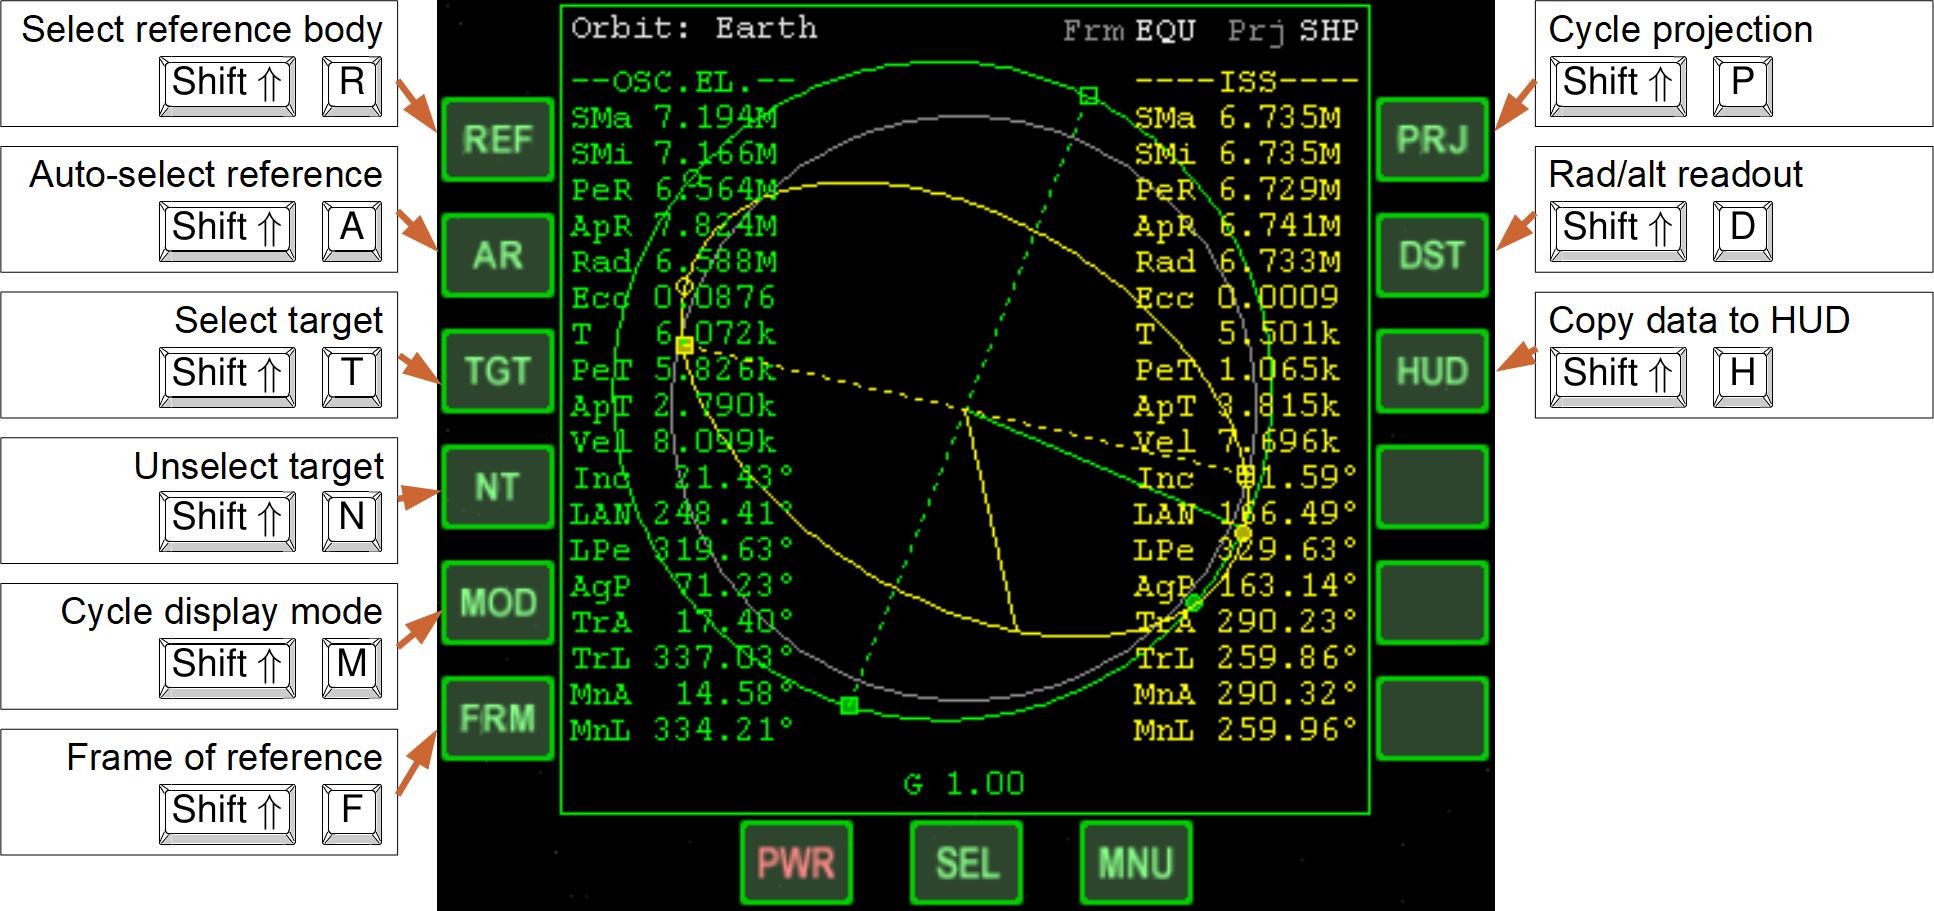
\includegraphics[width=0.99\hsize]{orbit_input.png}
\end{figure}

\noindent
\\
\textbf{MFD display components:}\\
\textbf{a) Graphic display mode}

\begin{figure}[H]
  \centering
  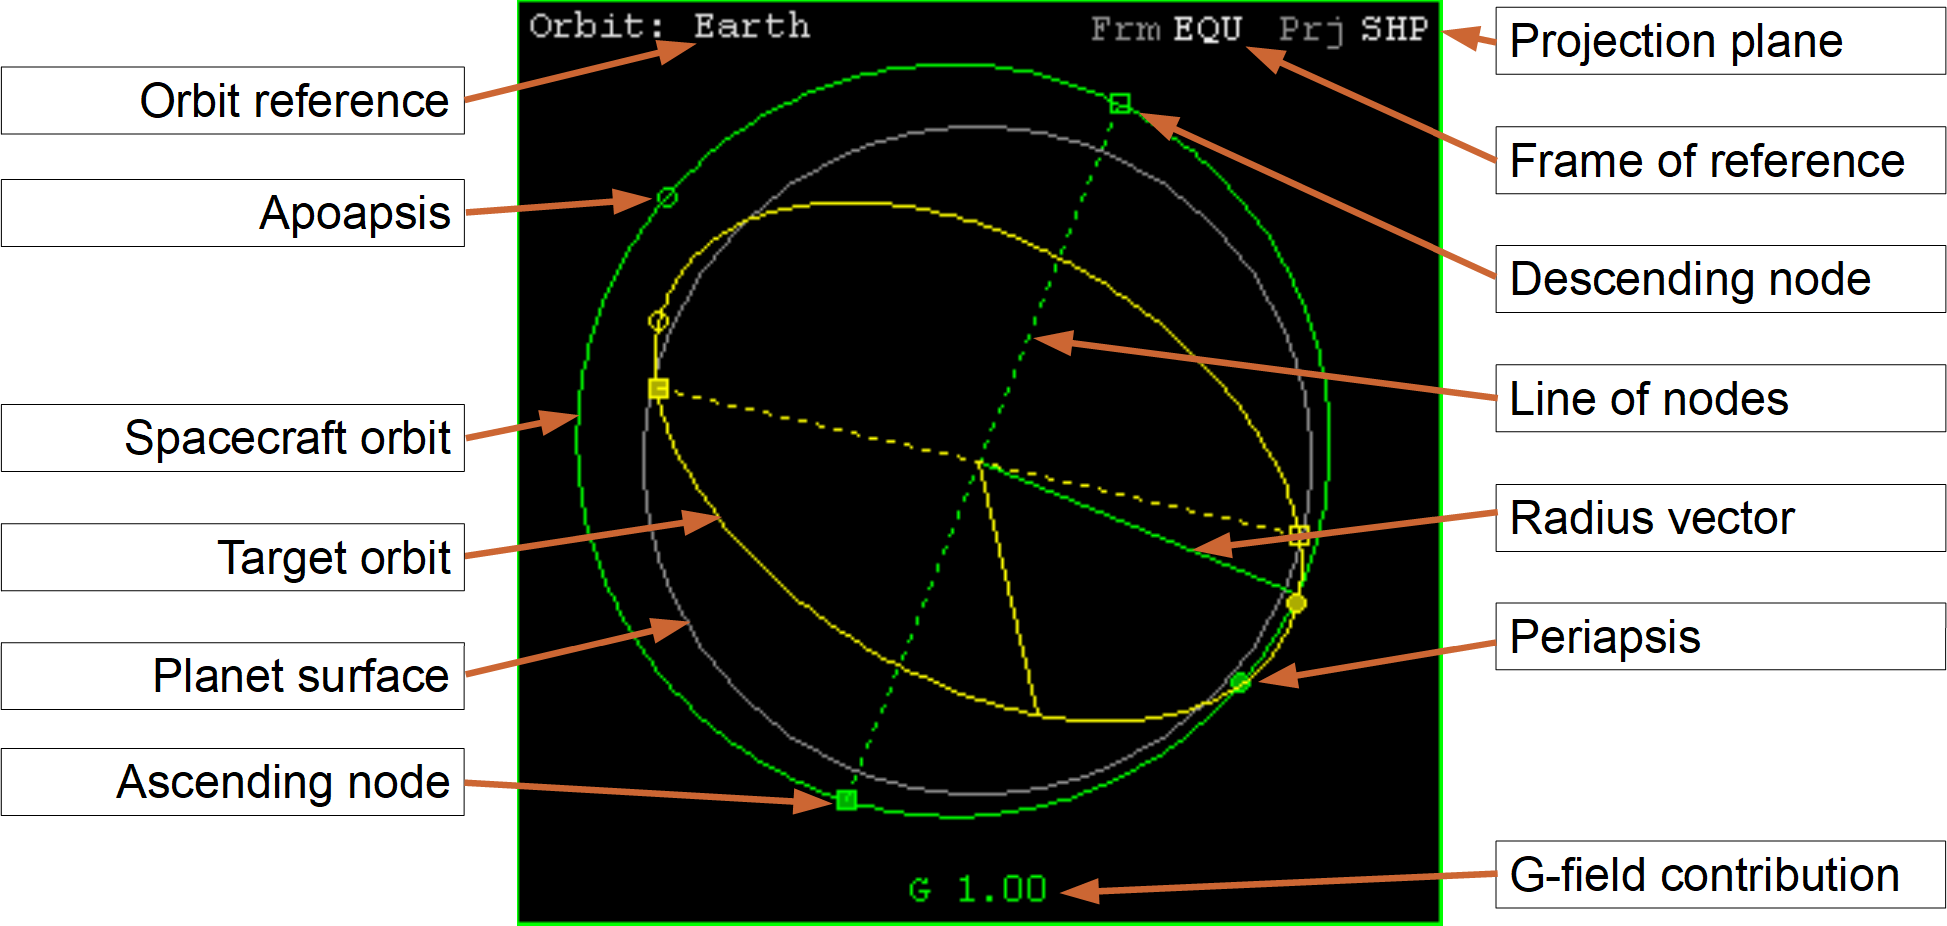
\includegraphics[width=0.99\hsize]{orbit_layout_1.png}
\end{figure}

\noindent
In graphical mode, the Orbit MFD shows the ship's orbit (green) and optionally the orbit of a target object (yellow) around the reference body (surface represented by a grey circle). The display also shows the ship's and target's current positions (radius vectors), the periapses (lowest orbit points) and apoapses (highest points), and the ascending and descending nodes with respect to the reference plane.\\
The user can select the plane into which the orbit representations are projected.\\
\\
\textbf{b) Orbital element list mode}

\begin{figure}[H]
  \centering
  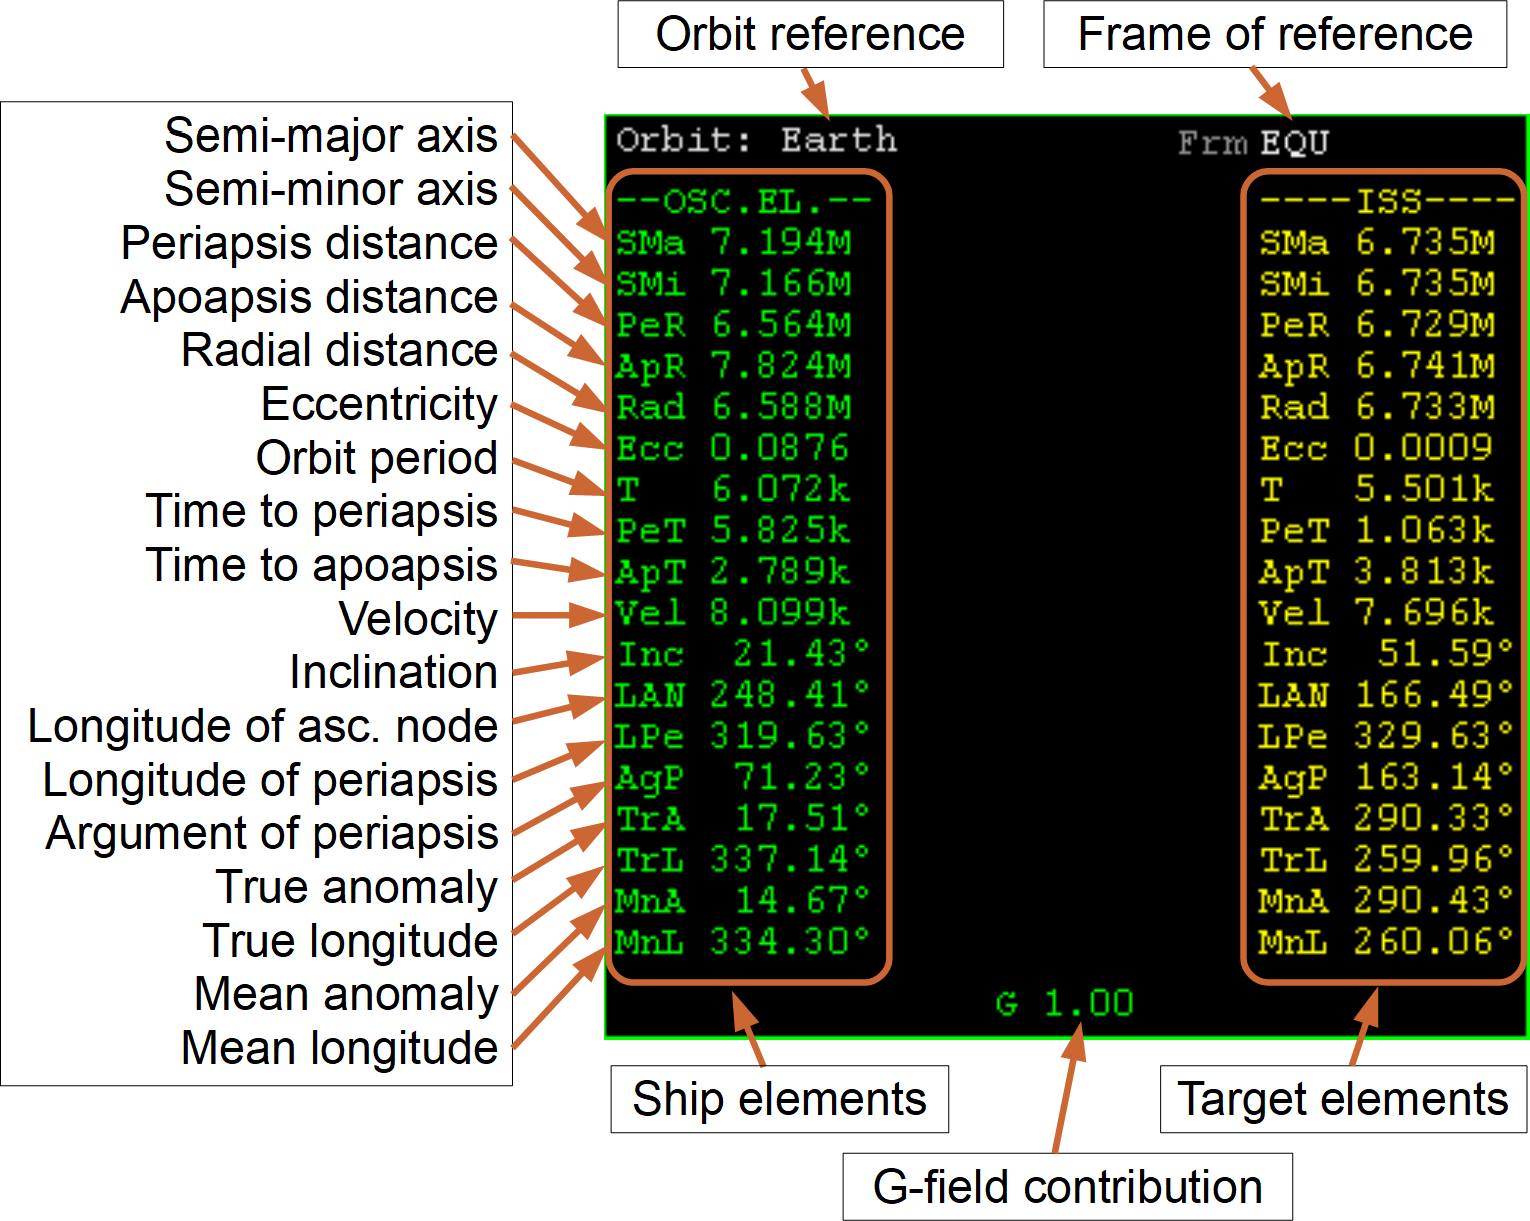
\includegraphics[width=0.75\hsize]{orbit_layout_2.png}
\end{figure}

\noindent
In list mode, the ship's orbital elements and other orbital parameters are listed in a column down the left side of the display (green). If a target is selected, its elements are listed on the right (yellow). The elements refer to the selected frame of reference, so they will change when switching between ecliptic (ECL) and equatorial (EQU) frame.\\
\\
\textbf{Notation:}

\begin{itemize}
\item Semi-major axis: the longest semi-diameter of the orbit ellipse
\item Semi-minor axis: the shortest semi-diameter of the orbit ellipse
\item Periapsis: the lowest point of the orbit (For Earth orbits, this is also called perigee. For solar orbits, this is also called perihelion.)
\item Apoapsis: the highest point of the orbit (For Earth orbits, this is also called apogee. For solar orbits, this is also called aphelion.)
\item Line of nodes: the intersection line of the orbital plane with the reference plane
\item Ascending node: the point at which the orbit passes through the reference plane from below
\item Descending node: the point at which the orbit passes through the reference plane from above
\item Radius vector: the line from the orbit's focus to the current position of the orbiting body
\end{itemize}

\noindent
For further explanation of orbital elements see section \ref{ssec:sol_orb_mech}.\\
For hyperbolic (non-periodic) orbits, the following parameters are interpreted specially:

\begin{itemize}
\item SMa: real semi-axis \textit{a}: distance from coordinate origin (defined by the intersection of the asymptotes of the hyperbola) to periapsis. The semi-major axis is displayed negative in this case.
\item SMi: imaginary semi-axis $b = a \sqrt{e^{2} - 1}$
\item ApD: apoapsis distance: not applicable
\item T: orbit period: not applicable
\item PeT: time to periapsis: negative after periapsis passages
\item ApT: time to apoapsis: not applicable
\item MnA: mean anomaly, defined as $M = e \cdot sinh(E) - E$, with \textit{E} hyperbolic eccentric anomaly
\end{itemize}

\noindent
\textbf{G-field contribution}\\
The G value at the bottom of the display shows the relative contribution of the current reference body to the total gravity field at the ship's position. This can be used to estimate the reliability of the Keplerian (2-body) orbit data displayed in the MFD. For values close to 1, a 2-body approximation is accurate. For low values the true orbit will deviate from the analytic calculation, resulting in a change of the osculating elements over time.\\
As a warning indicator, the G display will turn yellow for contributions < 0.8, and red if the selected reference body is not the dominant contributor to the gravity field. In that case, AR (\Shift\keystroke{A}) will select the dominant body.



\subsection{Align Orbital Plane}
\label{ssec:mfd_align}
This MFD mode aids in rotating the orbital plane in space so that it matches a target plane, e.g. the orbital plane of another object. The instrument displays the relevant orbital elements (inclination and longitude of the ascending node) of the current and target objects. It also shows the relative inclination (the angle between the two planes), the angles between the current target vector and the ascending and descending nodes, the time to intercept the next node, and the predicted required thruster burn time. See section \ref{ssec:basic_plane} on an introduction to plane change and how to use this MFD mode effectively.\\
The target plane can either be defined in terms of the orbital elements of another orbiting object, or by explicitly entering the required elements (inclination and longitude of the ascending node with respect to the ecliptic frame of reference).\\
\\
\textbf{Key options:}

%\begin{table}[H]
	%\centering
	\begin{longtable}{ |p{0.15\textwidth}|p{0.15\textwidth}|p{0.6\textwidth}| }
	\hline\rule{0pt}{2ex}
	\textbf{Button} & \textbf{Shortcut} & \textbf{Action}\\
	\hline\rule{0pt}{2ex}
	REF & \Shift\keystroke{R} & Select reference body\\
	\hline\rule{0pt}{2ex}
	AR & \Shift\keystroke{A} & Auto-reference\\
	\hline\rule{0pt}{2ex}
	TGT & \Shift\keystroke{T} & Input a new target orbit or target orbital parameters\\
	\hline\rule{0pt}{2ex}
	ELS & \Shift\keystroke{E} & Input target plane as ecliptic inclination and longitude of ascending node\\
	\hline\rule{0pt}{2ex}
	MOD & \Shift\keystroke{M} & Cycle display modes auto $\rightarrow$ orbit $\rightarrow$ ballistic $\rightarrow$ surface\\
	\hline
	\end{longtable}
%\end{table}

\noindent
\textbf{MFD control layout:}

\begin{figure}[H]
  \centering
  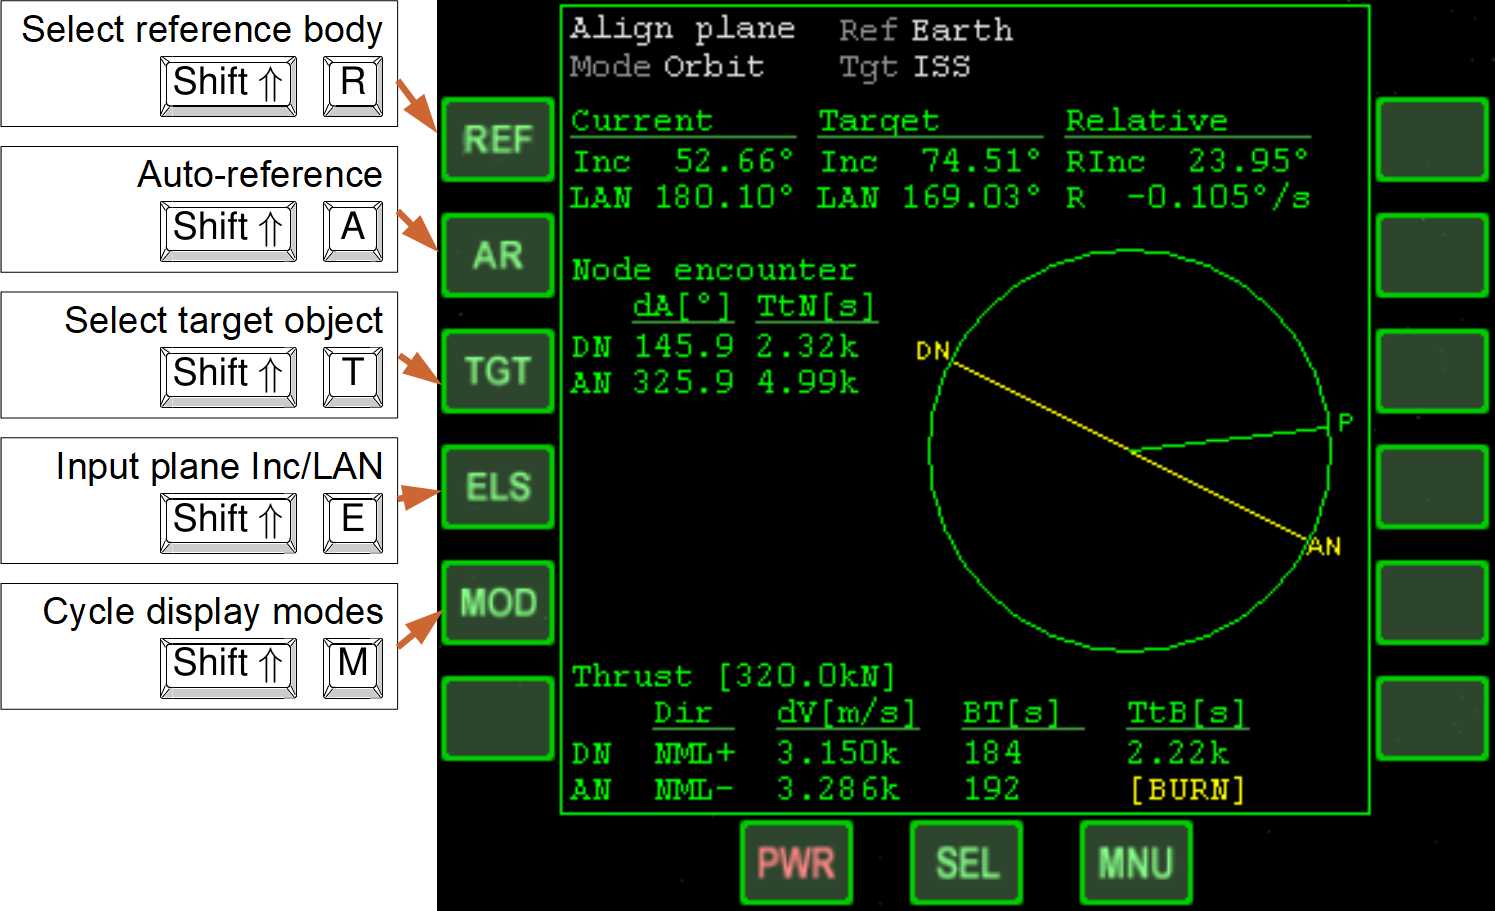
\includegraphics[width=0.75\hsize]{align_input.png}
\end{figure}

\noindent
\textbf{MFD display components:}\\
The Align-plane MFD mode can be used in two distinct situations

\begin{itemize}
\item while in orbit, to rotate the orbital plane to a target orientation
\item while on the ground, to find the optimal launch window for matching a target plane
\end{itemize}

\begin{figure}[H]
  \centering
  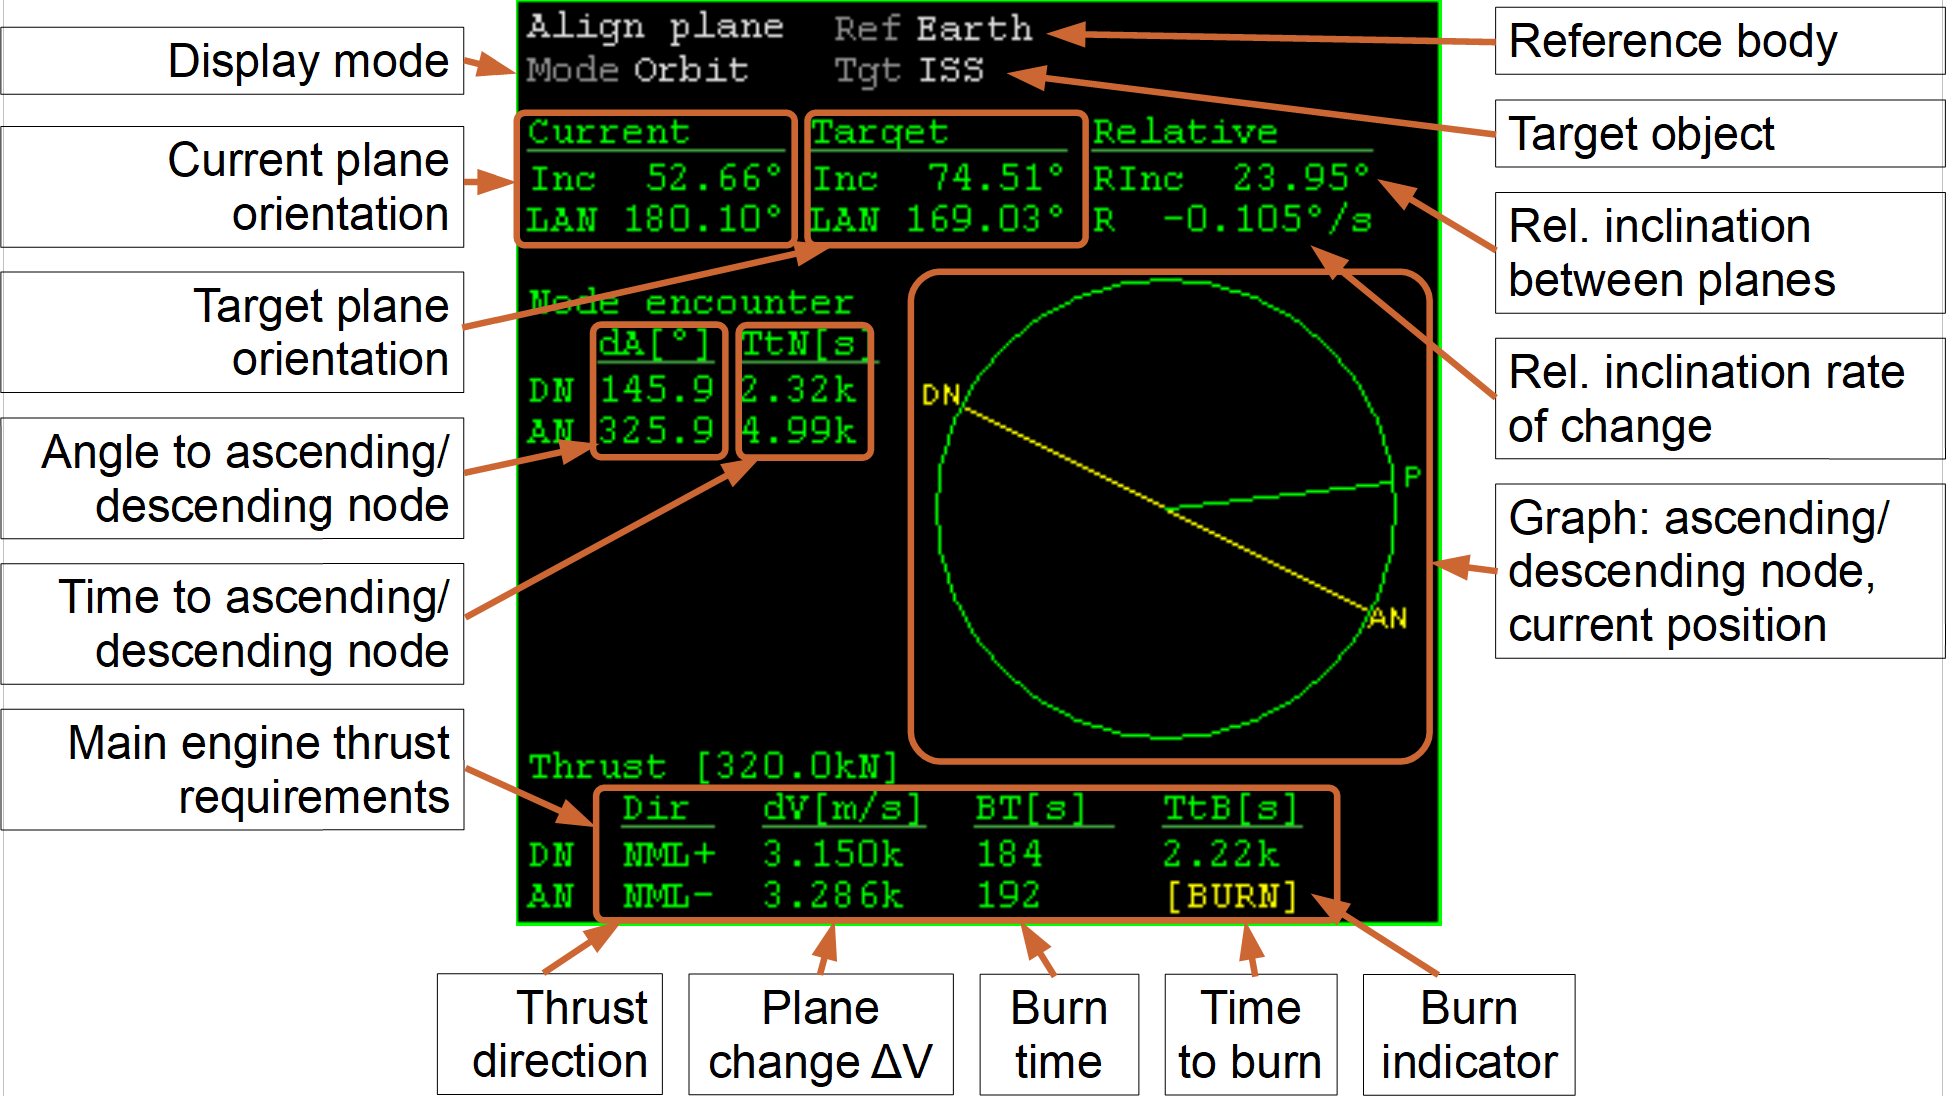
\includegraphics[width=0.99\hsize]{align_layout_1.png}
\end{figure}

\noindent
The two modes make different assumptions about the vessel trajectory. In \textit{orbit} mode, the vessel is assumed to follow its current osculating elements. The current and target planes always intersect, and the reference body's centre of mass always lies on the line of nodes.\\
In \textit{surface} mode, the vessel is expected to spin with the reference body at its current surface-relative position. Its trajectory is therefore on a plane parallel to the reference body's equator. It only intersects the target plane if the current latitude is lower than the target plane's inclination against the equator.\\
In addition, a \textit{ballistic} mode is supported. This is useful in transition from the surface to orbit, while the periapsis of the orbit constructed from the vessel's state vectors is still below the surface. In this mode, the orbit prediction is modified by altering the semi-major axis and eccentricity values such that the periapsis is on the planet surface, and the entire orbit is above ground. This mode provides more realistic burn times than orbit mode, which uses the osculating elements directly. Once the periapsis is above ground, orbit and ballistic mode are identical.\\
The user can select auto-mode to leave the mode selection to the software. In this case, surface mode is selected while the vessel is in contact with the surface, ballistic mode while the predicted periapsis is below surface, and orbit mode otherwise.\\
\\
\textbf{a) Orbit mode}

\begin{figure}[H]
  \centering
  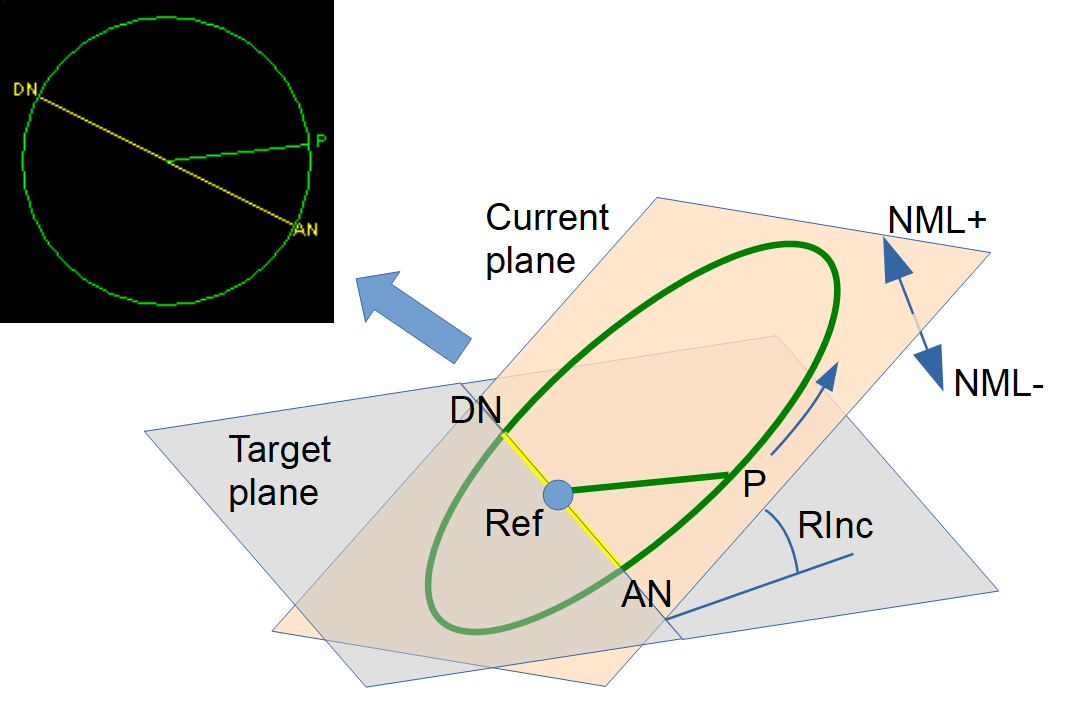
\includegraphics[width=0.75\hsize]{align_mode_a.png}
\end{figure}

\noindent
The current vessel and target plane orientations are shown in terms of two rotation angles in the ecliptic frame: Inc (inclination against the reference plane) and LAN (longitude of the ascending node - rotation of the ascending node against the vernal equinox).\\
The relative inclination between the planes and rate of change are also shown.\\
The \textit{Node encounter} data show the angles from the current position to the ascending and descending nodes (dA) and the times to the nodes (TtN).\\
The Thrust data show the required main engine burn parameters required for the plane change: thrust direction (Dir) - either normal (NML+) or anti-normal (NML-) to the current plane orientation, required velocity change (dV), required burn time (BT) and time to burn (TtB). The data are shown for plane change at the next ascending node (AN) or descending node (DN) passage.\\
\\
\textbf{b) Ballistic mode}

\begin{figure}[H]
  \centering
  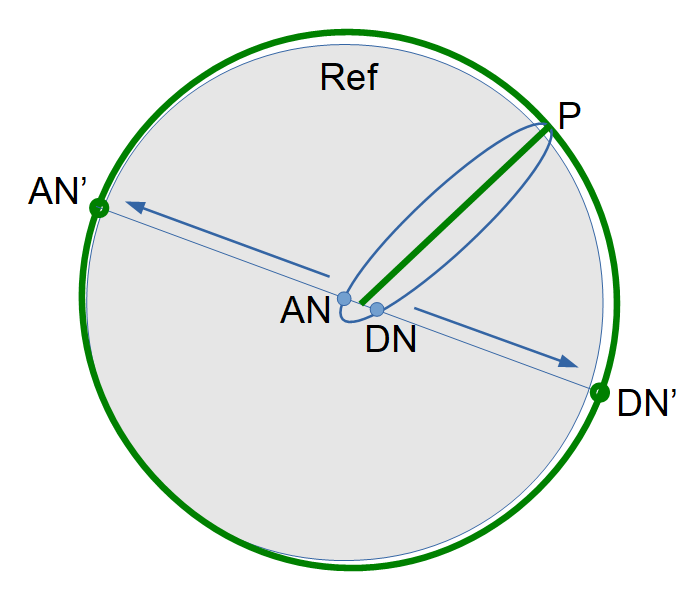
\includegraphics[width=0.5\hsize]{align_mode_b.png}
\end{figure}

\noindent
After launch, while the vessel's tangential velocity is low compared to circular orbital velocity, most of the orbit predicted from state vectors will be below surface, including the line of nodes, leading to inaccurate burn time predictions. In ballistic mode, the shape of the predicted orbit is altered by modifying the \textit{a} (semi-major axis) and \textit{e} (eccentricity) parameters such that the entire orbit is above the surface, with periapsis on the surface. The orientation of the orbital plane remains unchanged. This mode provides more realistic burn time predictions for a vessel in low altitude suborbital flight.\\
\\
\textbf{c) Surface mode}

\begin{figure}[H]
  \centering
  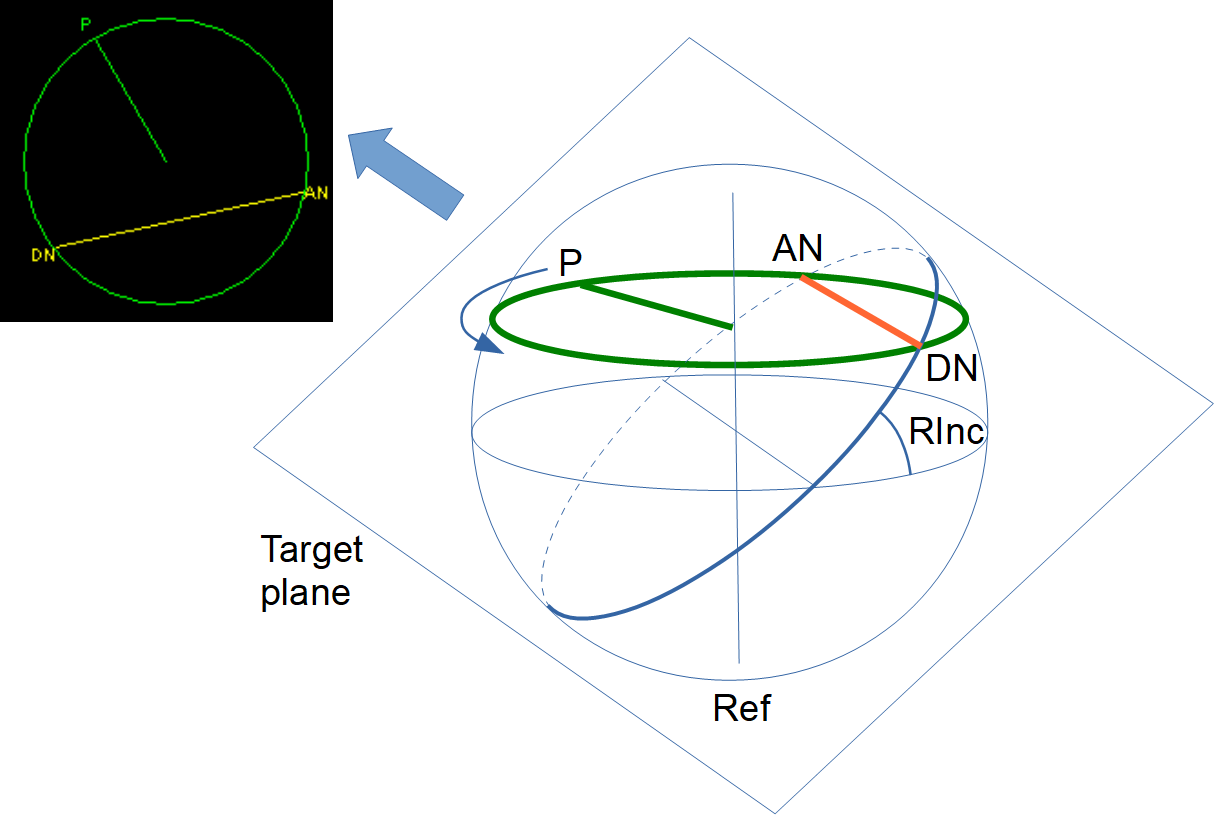
\includegraphics[width=0.75\hsize]{align_mode_c.png}
\end{figure}

\noindent
In surface mode, the vessel is assumed to remain at a fixed position at the planet surface. Its trajectory and velocity are defined by the planet radius and spin, and the latitude of the vessel position. These data are used to calculate the intersection (if any) with the target plane, the nodes, time to nodes and burn times.\\
The line of nodes in Surface mode is not displayed to go through the centre of the display, because the vessel trajectory will intersect the target plane only with a small arc (left image below), or not at all (right image below), depending on the latitude of the vessel position and the target plane inclination. If there is no intersection, the data in the MFD instead refer to the point of closest encounter (CE), the point of the vessel trajectory closest to the intersection of the two planes.

\begin{figure}[H]
  \centering
  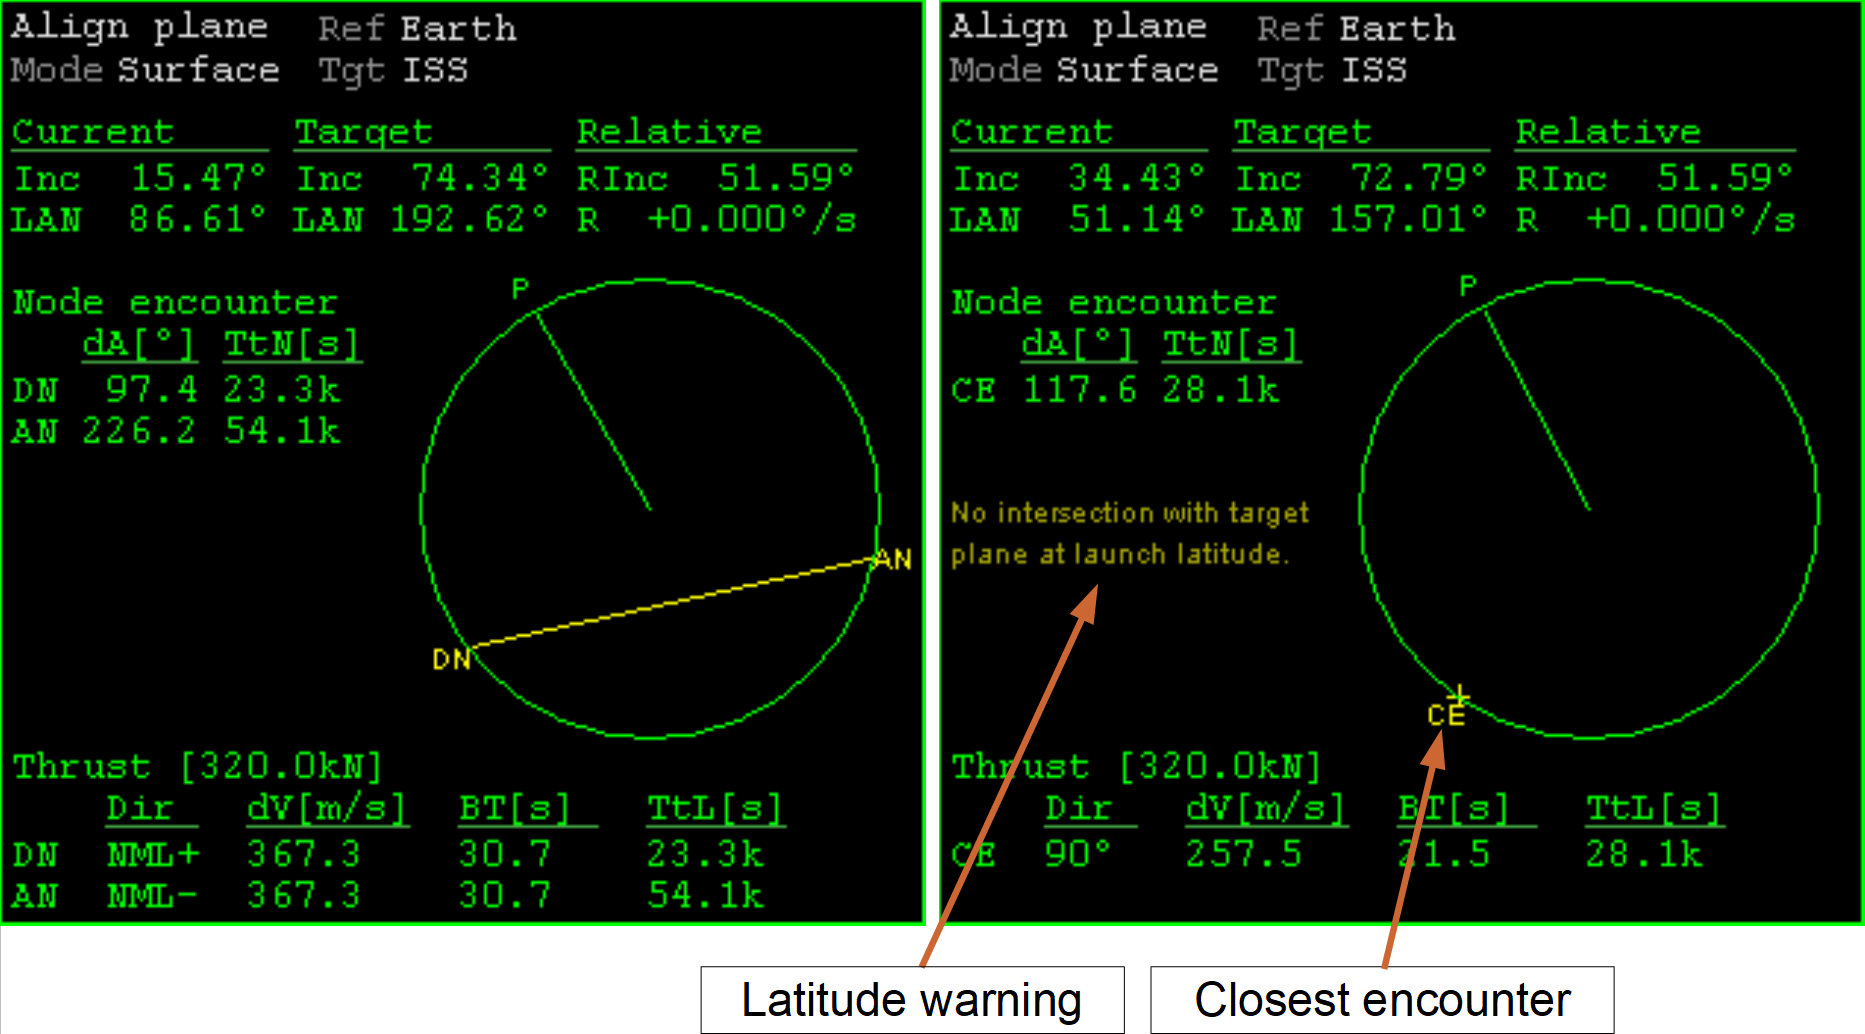
\includegraphics[width=0.99\hsize]{align_layout_2.png}
\end{figure}

\noindent
If the MFD is used in Orbit mode while the vessel is located on the surface, some of the readouts will show incorrect data because they refer to an unrealistic orbit constructed from the vessel's current state vectors which has the vessel at the apoapsis of a highly eccentric orbit with the periapsis close to the planet centre.


\subsection{Synchronise orbit}
The \textit{Synchronise Orbit} MFD mode assists in catching up with an orbiting body once the orbital planes have been aligned (see section \ref{ssec:mfd_align}).\\
The display shows the ship's and target body's orbits, together with a reference axis. It lists the times it will take both objects to reach this axis for a series of orbits.\\
For this mode to work properly, the orbital planes of both objects' orbits should be closely matched. The relative inclination between the two planes is shown in the lower left corner (RInc). If this becomes too large (e.g. > 1°), re-align the planes with the \textit{Align Orbital Planes} mode. Plane alignment and orbit synchronisation manoeuvres tend to take place at different positions of the orbit (plane alignment at the nodes, synchronisation at apoapsis/periapsis, so they can usually be queued without interfering with each other. Plane alignment burns are out-of-plane, while synchronisation burns are in-plane.\\
\\
\textbf{Key options:}

%\begin{table}[H]
	%\centering
	\begin{longtable}{ |p{0.15\textwidth}|p{0.15\textwidth}|p{0.6\textwidth}| }
	\hline\rule{0pt}{2ex}
	\textbf{Button} & \textbf{Shortcut} & \textbf{Action}\\
	\hline\rule{0pt}{2ex}
	TGT & \Shift\keystroke{T} & Select target object. Only objects orbiting the same body will be accepted.\\
	\hline\rule{0pt}{2ex}
	MOD & \Shift\keystroke{M} & Select reference axis mode. Intersection 1 and 2 are only available if the orbits intersect.\\
	\hline\rule{0pt}{2ex}
	LEN & \Shift\keystroke{N} & Select number of lines in the orbit timing list\\
	\hline\rule{0pt}{2ex}
	R- & \Shift\keystroke{,} & Rotate the reference axis counter-clockwise (manual mode only)\\
	\hline\rule{0pt}{2ex}
	R+ & \Shift\keystroke{.} & Rotate the reference axis clockwise (manual mode only)\\
	\hline
	\end{longtable}
%\end{table}

\noindent
\textbf{MFD control layout:}

\begin{figure}[H]
  \centering
  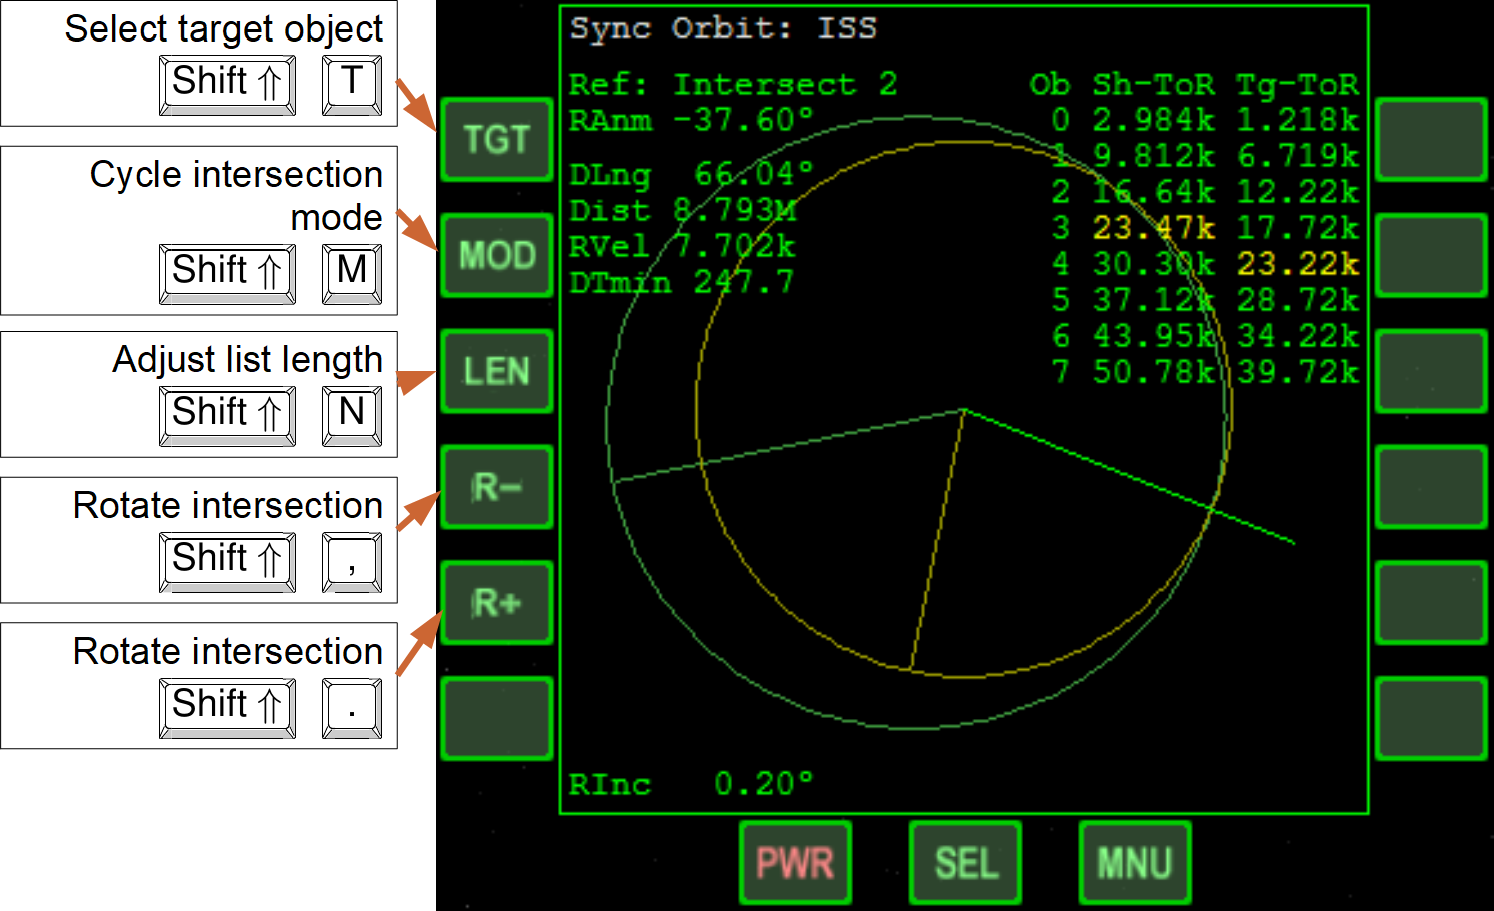
\includegraphics[width=0.75\hsize]{sync_input.png}
\end{figure}

\noindent
\textbf{MFD display components:}

\begin{figure}[H]
  \centering
  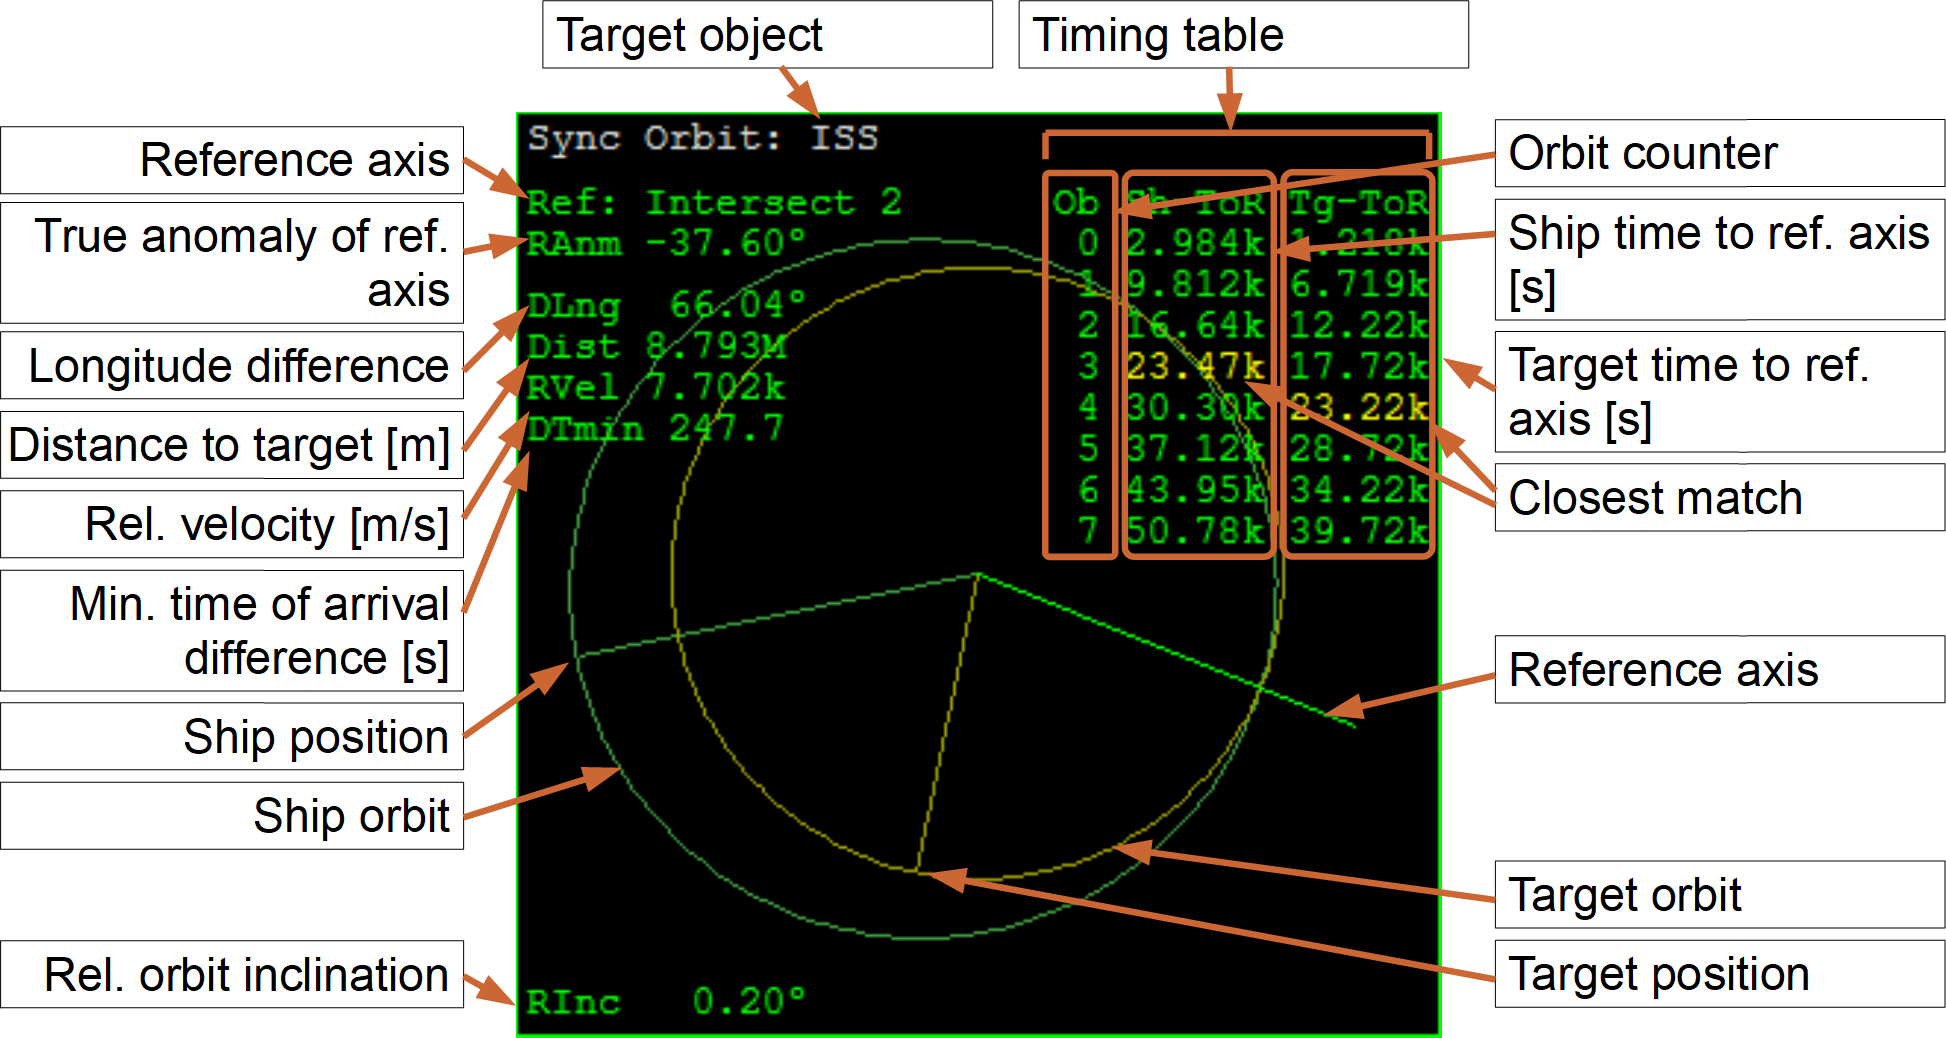
\includegraphics[width=0.99\hsize]{sync_layout.png}
\end{figure}


\begin{itemize}
\item \textbf{Target object:} The synchronisation target is displayed in the title line. It can be selected with \Shift\keystroke{T}.
\item \textbf{Reference axis:} A selectable axis for which the rendezvous timings are computed. Can be selected with \Shift\keystroke{M} from one of the following: orbit intersection 1 and 2 (if applicable), ship and target apoapsis and periapsis, and manual. The manual axis can be rotated \Shift\keystroke{,} and \Shift\keystroke{.}.
\item \textbf{True anomaly of ref. Axis (RAnm):} The angle between the reference axis and the ship's periapsis direction.
\item \textbf{Longitude difference (DLng):} The angle between ship and target measured from the central body.
\item \textbf{Distance (Dist):} Linear distance between ship and target [m].
\item \textbf{Rel. velocity (RVel):} Relative velocity between ship and target [m/s].
\item \textbf{Time-of-arrival difference (DTmin):} The minimum time difference [s] between the ship's and target's arrival at the reference axis for any of the listed orbits (see below).
\item \textbf{Rel. orbit inclination (RInc):} Angle between ship's and target's orbital planes.
\item \textbf{Time-to-reference lists (Sh-ToR and Tg-ToR):} A list of time intervals for the ship and target to reach the reference axis for the next n orbits. (\textit{n} can be selected with \Shift\keystroke{N}). The closest matched pair of timings is indicated in yellow. The DTmin value refers to this pair.
\end{itemize}

\noindent
See also section \ref{ssec:basic_sync} on some basic concepts for orbit synchronisation.


\subsection{Docking}
The \textit{Docking} MFD mode assists during final approach to dock with another vessel or orbital station. It provides indicators for translational and rotational alignment with the approach path, as well as distance and closing speed readouts.\\
This instrument relies on docking approach data received by your spacecraft from the target vessel. Approach data can be acquired in three different modes:

\begin{itemize}
\item IDS mode: Data are acquired from a radio signal sent by the docking target. The IDS (Instrument Docking System) signal is obtained by tuning a NAV receiver to the appropriate frequency and linking the Docking MFD to that receiver. The typical range for IDS is $\sim$20 km. To select a NAV receiver, press \Shift\keystroke{N}. The selected frequency is displayed in the upper right corner of the MFD.
\item Visual mode: Docking parameters are required from onboard visual systems (typically video cameras mounted in the docking port). The visual system aids in docking with targets that do not provide IDS. The typical range for visual mode is $\sim$100 m. To switch to visual mode, press \Shift\keystroke{V}.
\item Direct target selection: If you want to avoid the need to tune into a navigation transmitter signal, you can select a target directly (\Shift\keystroke{T}) by entering the target name and optional docking port index $\geq$ 1. (This shortcut method may be dropped in a future version.)
\end{itemize}

\noindent
Apart from their different operational range, the three modes provide identical data output on the MFD display.\\
While out of range of an IDS transmitter, the MFD can also be linked to the target vessel's long range transponder (XPDR) signal. This typically has a range of 1000 km, but only provides distance data, no alignment information.\\
\\
\textbf{Key options:}

%\begin{table}[H]
	%\centering
	\begin{longtable}{ |p{0.15\textwidth}|p{0.15\textwidth}|p{0.6\textwidth}| }
	\hline\rule{0pt}{2ex}
	\textbf{Button} & \textbf{Shortcut} & \textbf{Action}\\
	\hline\rule{0pt}{2ex}
	DCK & \Shift\keystroke{D} & Select local docking port. Only available if the vessel has more than one docking port.\\
	\hline\rule{0pt}{2ex}
	NAV & \Shift\keystroke{N} & Select NAV receiver for data input\\
	\hline\rule{0pt}{2ex}
	VIS & \Shift\keystroke{V} & Switch to visual docking data acquisition mode\\
	\hline\rule{0pt}{2ex}
	TGT & \Shift\keystroke{T} & Direct target and docking port selection\\
	\hline\rule{0pt}{2ex}
	SCL & \Shift\keystroke{S} & Toggle display resolution (coarse/fine) in the aiming reticle and radial scales.\\
	\hline\rule{0pt}{2ex}
	HUD & \Shift\keystroke{H} & Set HUD to Docking mode and copy data from MFD to HUD\\
	\hline
	\end{longtable}
%\end{table}

\noindent
\textbf{MFD control layout:}

\begin{figure}[H]
  \centering
  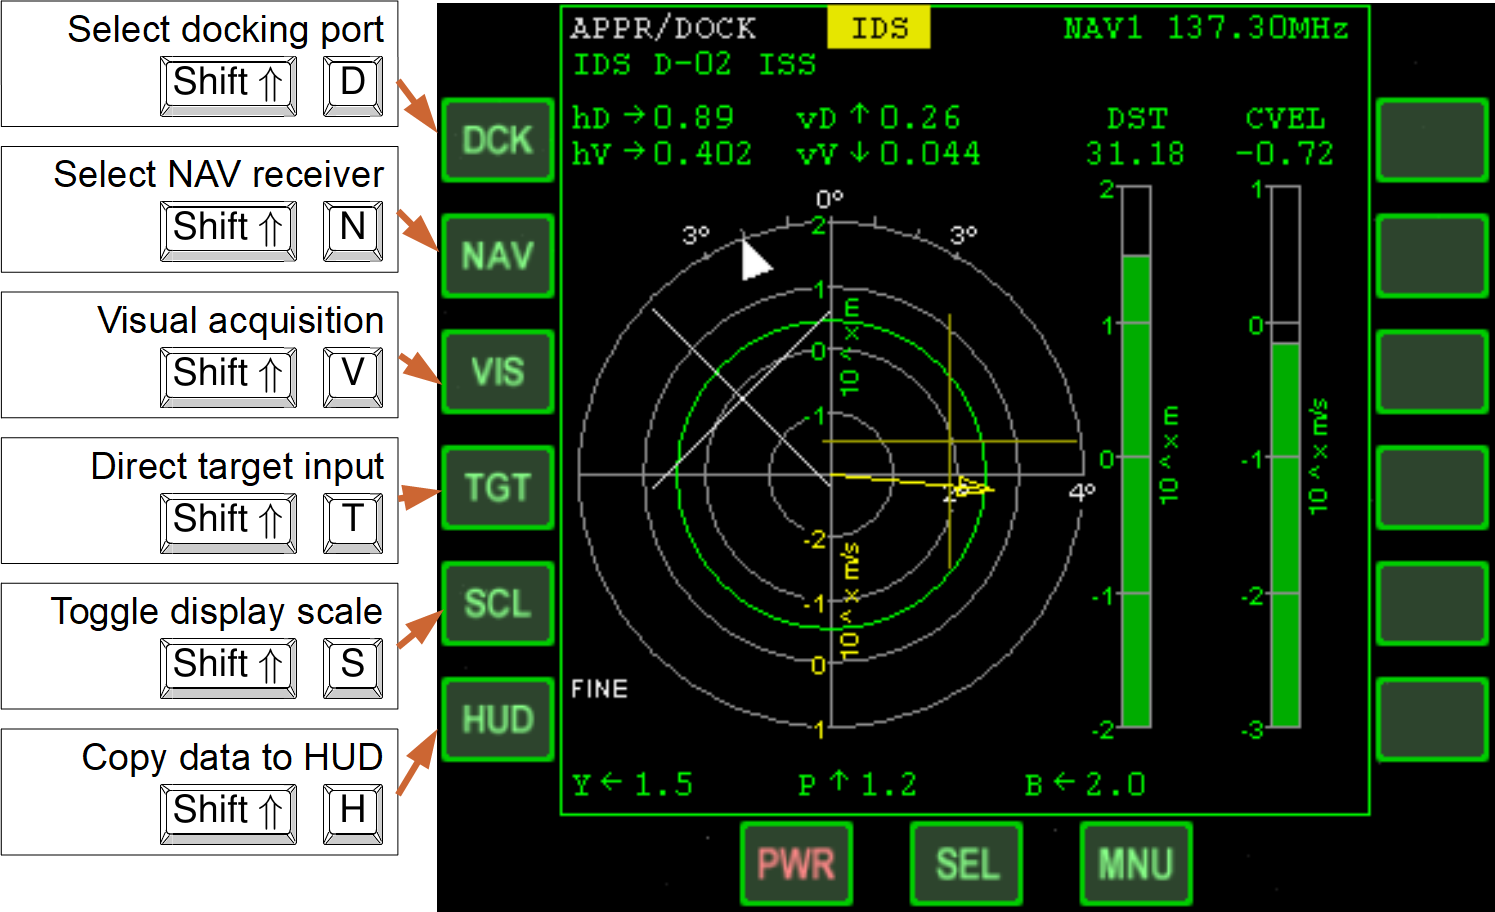
\includegraphics[width=0.75\hsize]{dock_input.png}
\end{figure}

\noindent
\textbf{MFD display components:}

\begin{figure}[H]
  \centering
  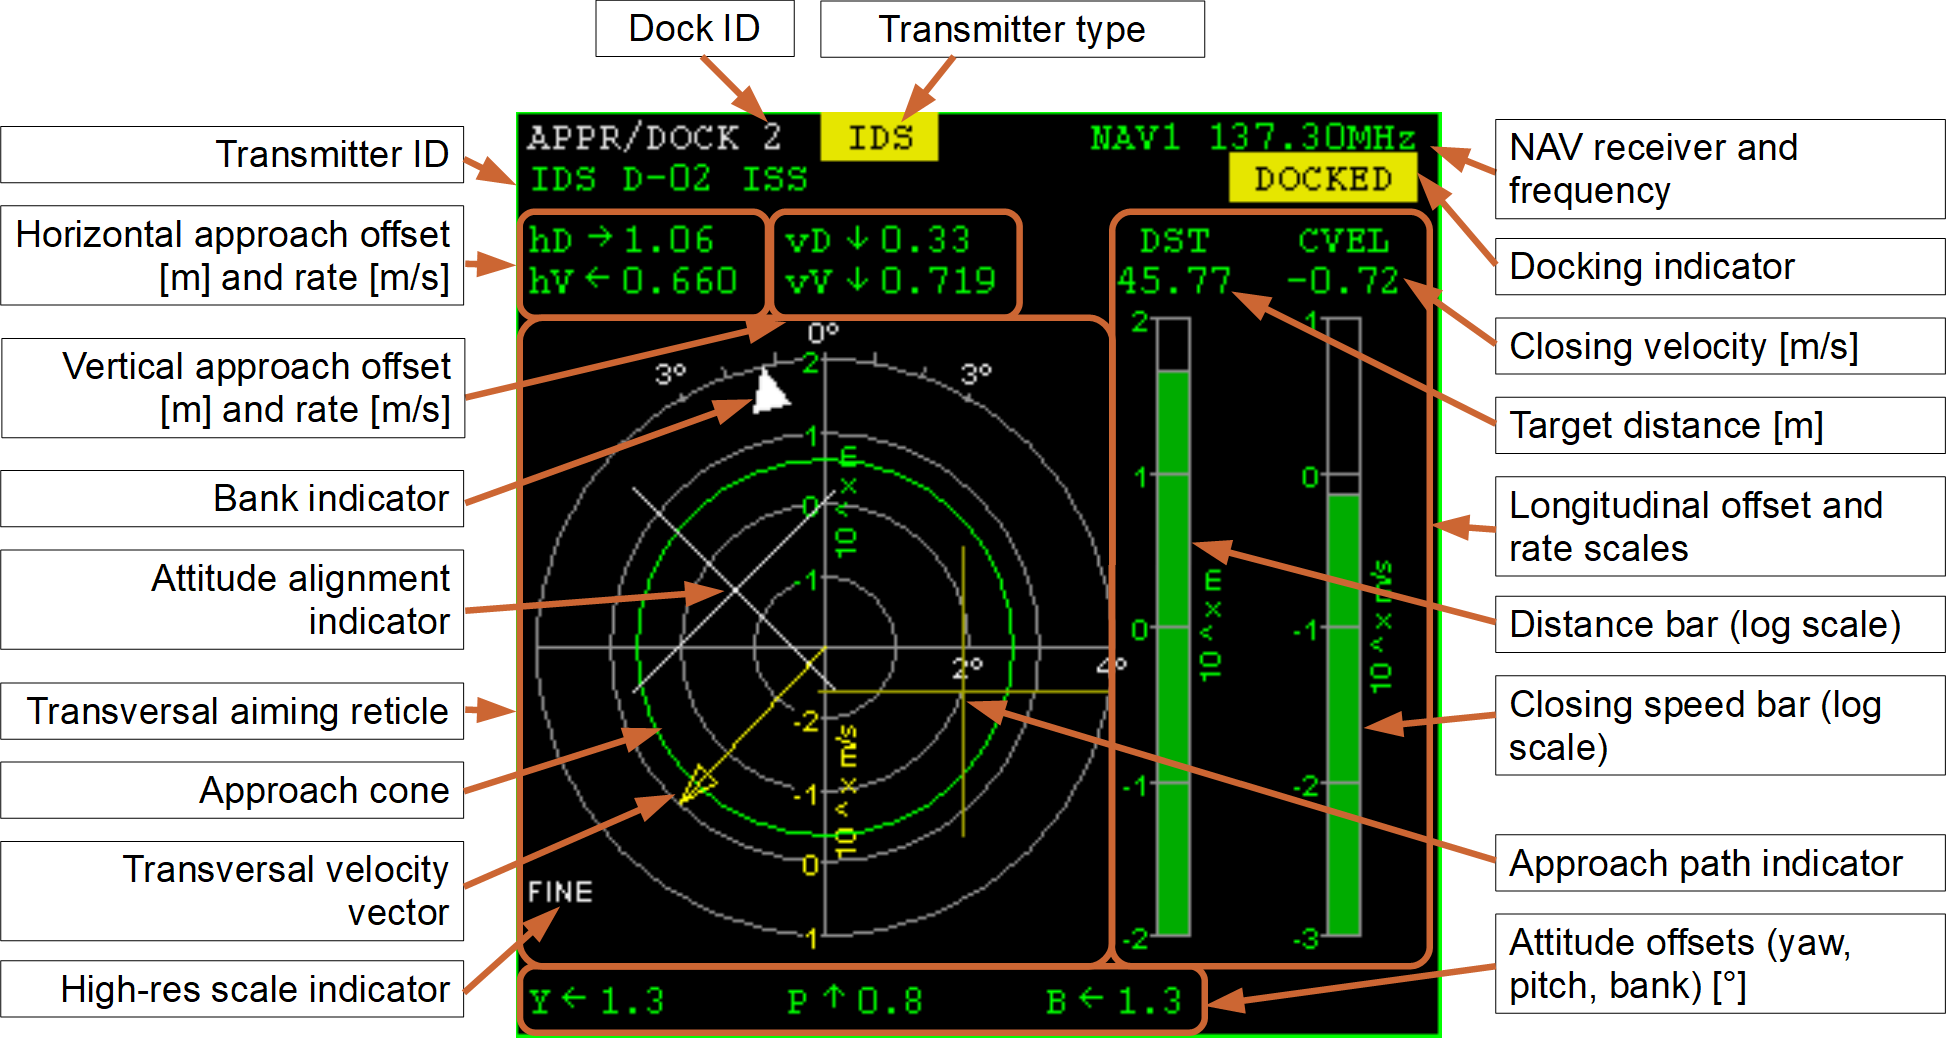
\includegraphics[width=0.99\hsize]{dock_layout.png}
\end{figure}

\noindent
The top two lines of the display contain information about the selected local docking port (dock ID, only applicable if the vessel has more than one port) and signal status of the targeted docking port on the remote vessel (the linked NAV receiver ID and its frequency setting, the type and identifying string of the received signal, if any). Also shown is the docking indicator (DOCKED) once the docking connection has been established.


\begin{itemize}
\item \textbf{Dock ID:} Identifies the docking port for which the instrument is computing approach parameters. Only applicable if the vessel has more than one docking port.
\item \textbf{Transmitter type/transmitter ID:} Identifies the source of the currently received transmitter signal, if any. This can either be a long-range transponder (XPDR) or an instrument docking (IDS) sender on the target vessel.
\end{itemize}

\noindent
The left part of the display shows a circular aiming reticle which contains a visual representation of both the lateral displacement from the approach path and the rotational alignment with the target docking port.

\begin{itemize}
\item \textbf{Approach path indicator:} The upright cross (+) indicates the position of the approach path relative to the ship (at the centre of the reticle). When the indicator is centred in the display, the ship is located on the approach path. The radial scale is logarithmic in the range 0.1-1000 m (coarse) or 0.01-100 m (fine). Tangential alignment is performed with attitude thrusters in \textit{linear} mode (see section \ref{ssec:control_att}).
\item \textbf{Transversal velocity vector:} The yellow arrow indicates the relative tangential velocity of your vessel with respect to the target. The radial scale is logarithmic in the range 0.01-100 m/s (coarse) or 0.001-10 m/s (fine). If the relative velocity is below the lower range limits, the arrow is not shown. To move the vessel onto the approach path, engage RCS thrusters in linear configuration so that the arrow points towards the approach path indicator.
\item \textbf{Attitude alignment indicator:} The white or red $\times$ symbol indicates the alignment of the ship's docking port orientation with the approach path direction. When centred, the docking ports on the local and remote vessels are aligned in yaw and pitch. The symbol turns red if the misalignment is > 2.5°. The radial scale is linear in the range 0-20° (coarse) or 0-4° (fine). Rotational alignment is performed with RCS in rotational configuration (see section \ref{ssec:control_att}).
\item \textbf{Bank rotation indicator:} This arrow moves along the circumference of the reticle to indicate the ship's longitudinal (bank) alignment with the docking port. To align, the indicator must be moved into the 12 o'clock position (0°) by rotating the ship around its longitudinal axis, engaging bank attitude thrusters in rotational configuration (see section \ref{ssec:control_att}).When alignment is achieved, the indicator turns white (misalignment < 2.5°). Note that this indicator is only displayed when directional alignment (see above) is within 5°. The tick marks at the top of the aiming reticle represent 10° (coarse) or 1° (fine) misalignments.
\item \textbf{Approach cone:} The concentric green or red circle indicates the size of the approach cone at the current distance to the target dock. The ship should approach the dock so that the approach path indicator is always inside the approach cone (green). The approach cone cross section becomes smaller as the ship approaches the dock.
\end{itemize}

\noindent
The readouts above the reticle show the numerical values of the linear offsets and rates.

\begin{itemize}
\item \textbf{hD/vD:} Transversal (horizontal/vertical) displacements from the approach path [m]. These are the distances (projected into the plane normal to the approach path) of the current vessel position from the approach path. The arrows indicate the direction of the approach path from the vessel position. In the aiming reticle the offset from the approach path is graphically represented by the approach path indicator (+).
\item \textbf{hV/vV:} Transversal (horizontal/vertical) velocities relative to the approach path [m/s]. These are the velocity components relative to the target, projected into the plane normal to the approach path. The arrows indicate the velocity directions. If the velocity direction indicators match the offset direction indicators, the vessel is moving towards the approach path. In the aiming reticle the relative transversal velocity is represented by the transversal velocity vector.
\end{itemize}

\noindent
The readouts below the reticle show the rotational misalignment values.

\begin{itemize}
\item \textbf{Y/P/B:} Vessel attitude rotation from the required docking attitude (yaw/pitch/bank) [degrees]. The arrows indicate the directions in which the vessel must be rotated to align with the docking port orientation. This alignment is done in rotational RCS configuration. In the aiming reticle the attitude misalignments are represented by the attitude alignment indicator (yaw, pitch) and the bank rotation indicator.
\end{itemize}

\noindent
The scales in the right half of the display show the longitudinal distance and rate along the approach path direction.

\begin{itemize}
\item \textbf{DST:} dock-to-dock distance [m]. The bar shows the distance on a logarithmic scale in the range 0.1-1000 m (coarse) or 0.01-100 m (fine).
\item \textbf{CVEL:} Closing speed [m/s]. The bar shows the closing speed on a logarithmic scale in the range 0.01-100 m/s (coarse) or 0.001-10 m/s (fine). Yellow indicates positive closing speed.
\end{itemize}

\noindent
Closing speed should be reduced as the ship approaches the dock (using RCS in linear configuration). The relative velocity at contact should be < 0.1 m/s.\\
\\
\textbf{Notes:}

\begin{itemize}
\item To dock successfully you must approach the dock to within 0.3 m. Additional restrictions may be implemented in the future (speed, alignment, etc.)
\item No collision checks are currently performed. If you fail to dock and keep closing in, you may fly your ship through the target vessel.
\end{itemize}


\subsection{RCS Attitude}
The \textit{Attitude} MFD mode provides advanced functions for orbital attitude control beyond the built-in attitude modes (pro-/retrograde, normal/anti-normal). This MFD mode is an example for a script-driven MFD definition. To make it available, the \textit{ScriptMFD} module must be activated in the Launchpad Modules tab.\\
The attitude MFD mode operates by taking control of the vessel's RCS thrusters to orient it in the commanded attitude. This only works for vessels with a full RCS that allows alignment in all three vessel axes.\\
A new attitude mode is defined by first selecting a \textit{Base} mode and then adding additional rotations to it. Press SET to open the mode definition page. If an attitude mode is currently active, the definition page initially displays the parameters of this mode. Otherwise, a default prograde mode is shown. You can use the BAS button to cycle through the available base modes: \textit{prograde}, \textit{normal}, \textit{perpendicular} and \textit{radial}. Each mode can be inverted by pressing the INV button, e.g. prograde $\rightarrow$ retrograde, or normal $\rightarrow$ anti-normal, etc. The following table shows the orientation of each base mode from two principal vessel axes (forward, +\textbf{z}, and up, +\textbf{y}), relative to the orbital velocity vector (\textbf{v}), radius vector (\textbf{r}) and orbital plane normal (\textbf{n} = \textbf{r} $\times$ \textbf{v}).

%\begin{table}[H]
	%\centering
	\begin{longtable}{ |p{0.3\textwidth}|p{0.6\textwidth}| }
	\hline\rule{0pt}{2ex}
	\textbf{Mode} & \textbf{Vessel orientation}\\
	\hline\rule{0pt}{2ex}
	prograde & +z $\rightarrow$ +v, +y $\rightarrow$ +n\\
	\hline\rule{0pt}{2ex}
	retrograde & +z $\rightarrow$ -v, +y $\rightarrow$ -n\\
	\hline\rule{0pt}{2ex}
	normal & +z $\rightarrow$ +n, +y $\rightarrow$ -v\\
	\hline\rule{0pt}{2ex}
	antinormal & +z $\rightarrow$ -n, +y $\rightarrow$ -v\\
	\hline\rule{0pt}{2ex}
	perpendicular (in) & +z $\rightarrow$ -v $\times$ n, +y $\rightarrow$ +v\\
	\hline\rule{0pt}{2ex}
	perpendicular (out) & +z $\rightarrow$ +v $\times$ n, +y $\rightarrow$ -v\\
	\hline\rule{0pt}{2ex}
	radial (down) & +z $\rightarrow$ -r, +y $\rightarrow$ +v\\
	\hline\rule{0pt}{2ex}
	radial (up) & +z $\rightarrow$ +r, +y $\rightarrow$ -v\\
	\hline
	\end{longtable}
%\end{table}

\noindent
After defining the base mode, additional rotations can be added to modify the vessel orientation. Press the +R button to add a rotation. You can select a rotation axis (pitch, yaw, roll) by pressing the AX button. Set a rotation angle with the +V and -V buttons. You can add multiple rotations, but note that the order is significant. Rotations do not commute. You can select a rotation with the UP and DN buttons. Rotations can be deleted with the -R button.\\
When the mode definition is complete, press the GO button to activate it. You can continue editing the mode, and activate the modifications by pressing GO again. To return to the main page, press RTN.\\
\\
\textbf{Key options:}

%\begin{table}[H]
	%\centering
	\begin{longtable}{ |p{0.15\textwidth}|p{0.15\textwidth}|p{0.6\textwidth}| }
	\hline\rule{0pt}{2ex}
	\textbf{Button} & \textbf{Shortcut} & \textbf{Action}\\
	\hline
	\multicolumn{3}{|c|}{\rule{0pt}{2ex}\textbf{\textit{Main page:}}}\\
	\hline\rule{0pt}{2ex}
	SET & \Shift\keystroke{S} & Set/adjust attitude mode\\
	\hline\rule{0pt}{2ex}
	DCK & \Shift\keystroke{D} & Switch to docking alignment mode\\
	\hline\rule{0pt}{2ex}
	SUS & \Shift\keystroke{P} & Suspend/activate attitude mode\\
	\hline\rule{0pt}{2ex}
	END & \Shift\keystroke{X} & Cancel active attitude mode\\
	\hline\rule{0pt}{2ex}
	CFG & \Shift\keystroke{C} & Define offset angles for default attitude modes\\
	\hline
	\multicolumn{3}{|c|}{\rule{0pt}{2ex}\textbf{\textit{Attitude definition page:}}}\\
	\hline\rule{0pt}{2ex}
	BAS & \Shift\keystroke{B} & Cycle through attitude base modes\\
	\hline\rule{0pt}{2ex}
	INV & \Shift\keystroke{I} & Invert current base mode\\
	\hline\rule{0pt}{2ex}
	CUR & \Shift\keystroke{K} & Bind target mode to current attitude\\
	\hline\rule{0pt}{2ex}
	+R & \Shift\keystroke{A} & Add a rotation to the base mode\\
	\hline\rule{0pt}{2ex}
	-R & \Shift\keystroke{X} & Delete the currently selected rotation\\
	\hline\rule{0pt}{2ex}
	+V & \Shift\keystroke{.} & Increase the angle of the currently selected rotation\\
	\hline\rule{0pt}{2ex}
	-V & \Shift\keystroke{,} & Decrease the angle of the currently selected rotation\\
	\hline\rule{0pt}{2ex}
	AX & \Shift\keystroke{C} & Cycle through rotation axes for currently selected rotation\\
	\hline\rule{0pt}{2ex}
	UP & \Shift\keystroke{U} & Switch to the previous rotation\\
	\hline\rule{0pt}{2ex}
	DN & \Shift\keystroke{D} & Switch to the next rotation\\
	\hline\rule{0pt}{2ex}
	GO & \Shift\keystroke{Q} & Activate the attitude mode\\
	\hline\rule{0pt}{2ex}
	RTN & \Shift\keystroke{R} & Return to main page\\
	\hline
	\multicolumn{3}{|c|}{\rule{0pt}{2ex}\textbf{\textit{Docking alignment page:}}}\\
	\hline\rule{0pt}{2ex}
	NAV & \Shift\keystroke{N} & Cycle through NAV receiver stack\\
	\hline\rule{0pt}{2ex}
	ACT & \Shift\keystroke{A} & Activate dock alignment mode\\
	\hline\rule{0pt}{2ex}
	CNC & \Shift\keystroke{X} & Cancel docking alignment mode\\
	\hline\rule{0pt}{2ex}
	RTN & \Shift\keystroke{R} & Return to main page\\
	\hline
	\multicolumn{3}{|c|}{\rule{0pt}{2ex}\textbf{\textit{Offset configuration page:}}}\\
	\hline\rule{0pt}{2ex}
	+R & \Shift\keystroke{A} & Add a new rotation offset\\
	\hline\rule{0pt}{2ex}
	-R & \Shift\keystroke{X} & Delete the currently selected rotation offset\\
	\hline\rule{0pt}{2ex}
	AX & \Shift\keystroke{C} & Cycle through rotation axes for currently selected rotation\\
	\hline\rule{0pt}{2ex}
	+V & \Shift\keystroke{.} & Increase angle for currently selected rotation\\
	\hline\rule{0pt}{2ex}
	-V & \Shift\keystroke{,} & Decrease angle for currently selected rotation\\
	\hline\rule{0pt}{2ex}
	UP & \Shift\keystroke{U} & Switch to previous rotation\\
	\hline\rule{0pt}{2ex}
	DN & \Shift\keystroke{D} & Switch to next rotation\\
	\hline\rule{0pt}{2ex}
	GO & \Shift\keystroke{Q} & Activate offset configuration\\
	\hline\rule{0pt}{2ex}
	RTN & \Shift\keystroke{R} & Return to main page\\
	\hline
	\end{longtable}
%\end{table}

\noindent
\textbf{MFD control layout (main page):}

\begin{figure}[H]
  \centering
  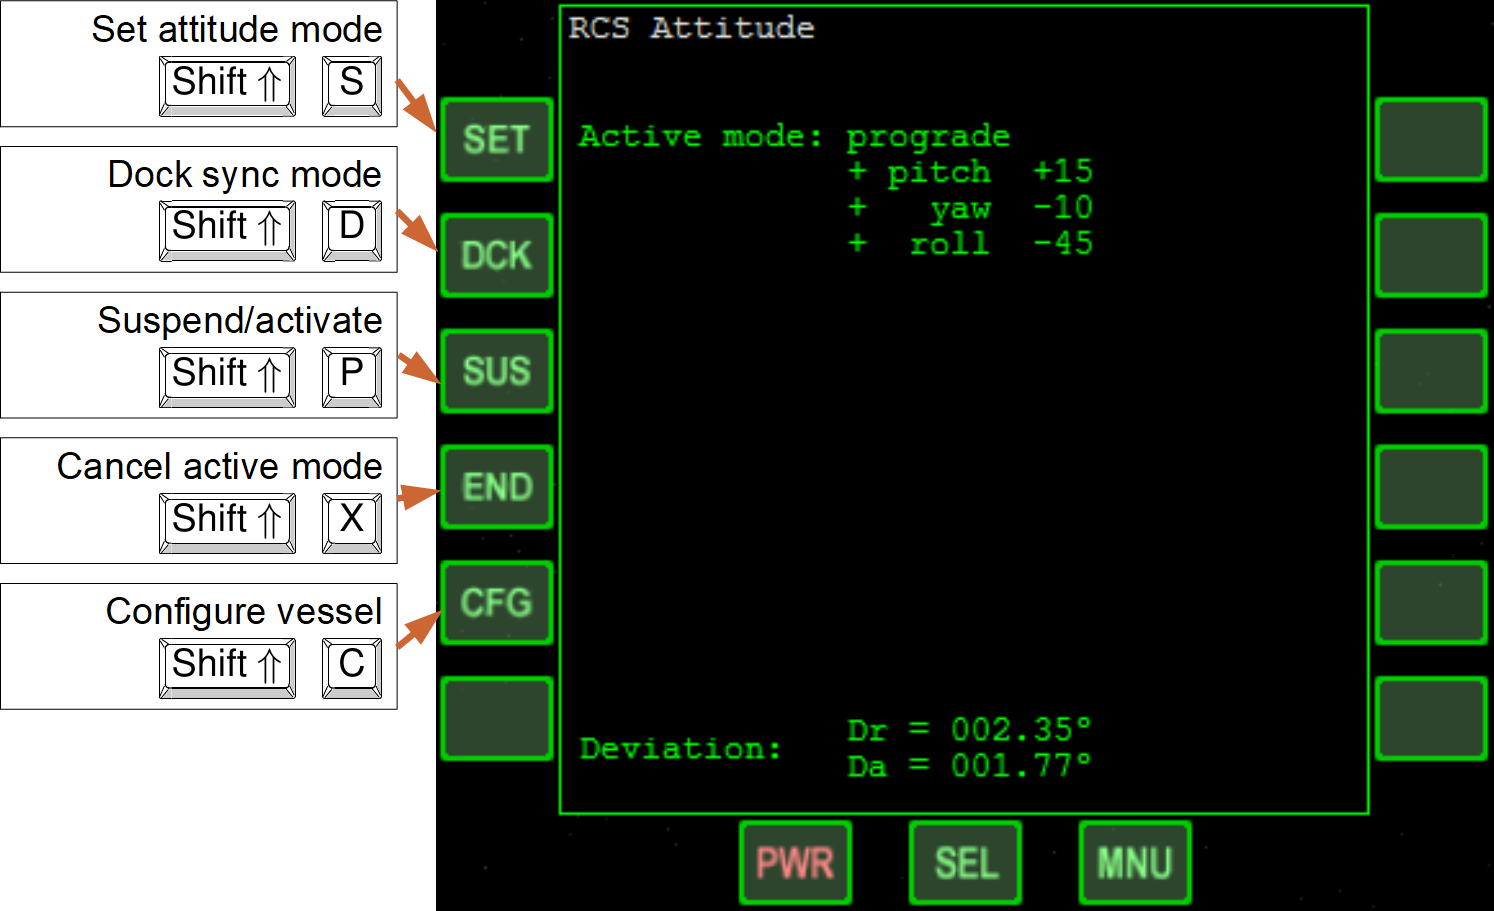
\includegraphics[width=0.75\hsize]{rcs_input.png}
\end{figure}

\noindent
\textbf{MFD display components (main page):}

\begin{figure}[H]
  \centering
  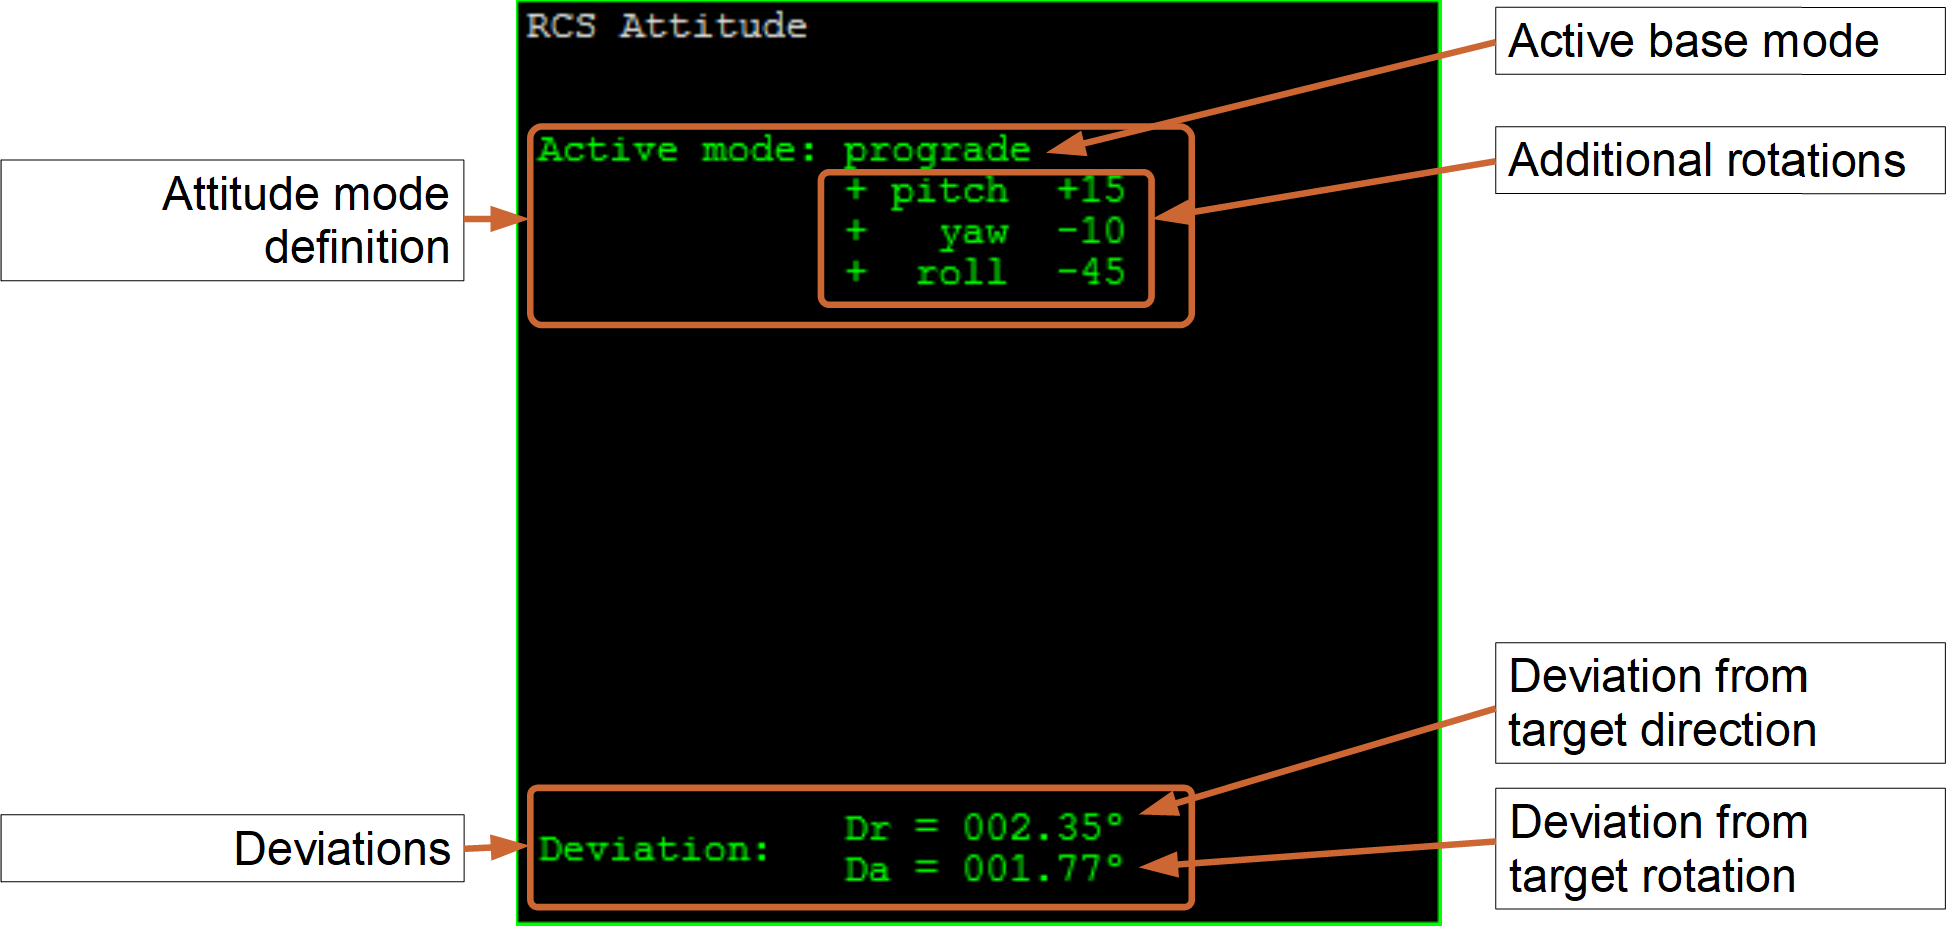
\includegraphics[width=0.99\hsize]{rcs_layout.png}
\end{figure}

\noindent
\textbf{Rotational docking alignment}\\
The Attitude MFD can also align the vessel with the target docking port orientation. From the main page, press the DCK button. This opens the Dock alignment page. Docking alignment is performed with data from an IDS (instrument docking system) transmitter. Make sure that one of your NAV radios is tuned to the IDS of the target dock. Use the NAV button to select the appropriate receiver from the stack. Docking alignment can only be activated once an IDS signal is received. Press ACT to activate the alignment mode. You can then return to the main page with RTN.\\
Docking alignment mode is cancelled if the IDS transmitter goes out of range, or if the NAV receiver is re-tuned.\\
Docking alignment also works for docking ports not oriented in the vessel's forward (+z) axis.\\
\\
\textbf{Pre-multiplying an angular offset}\\
Sometimes it is useful to apply an angular offset to all attitude modes. For example, the Space Shuttle's OMS engines are tilted by 15° against the longitudinal axis. The resulting thrust vector therefore points to -15° pitch. For a prograde OMS burn, the Shuttle needs to pitch up by 15° against the orbital velocity vector. This constant offset due to engine arrangement can be taken into account with the Attitude MFD.\\
Open the Configuration page by pressing CFG from the main page. You can now add angular offsets by pressing the ADD button. You can then set the rotation axis and angle similar to the attitude mode setup. For example for the Shuttle, add a pitch rotation of +15°. When done, press RTN to return to the main page. The additional offset will be added to all attitude modes, except for the docking alignment mode.


\subsection{Transfer}
\label{ssec:mfd_transfer}
The Transfer MFD mode is used for calculating transfer orbits between planets or moons (or more generally, between any objects with significantly different orbits, for which the Sync orbit MFD mode is not sufficient).\\
Note that Orbiter now contains Duncan Sharpe's TransX MFD mode as a plug-in module, which supersedes and extends most of the Transfer MFD functionality (see section \ref{ssec:mfd_transx}).\\
\\
\textbf{Key options:}

%\begin{table}[H]
	%\centering
	\begin{longtable}{ |p{0.15\textwidth}|p{0.15\textwidth}|p{0.6\textwidth}| }
	\hline\rule{0pt}{2ex}
	\textbf{Button} & \textbf{Shortcut} & \textbf{Action}\\
	\hline\rule{0pt}{2ex}
	REF & \Shift\keystroke{R} & Select the reference celestial body\\
	\hline\rule{0pt}{2ex}
	SRC & \Shift\keystroke{S} & Select the source object\\
	\hline\rule{0pt}{2ex}
	TGT- & \Shift\keystroke{T} & Select target\\
	\hline\rule{0pt}{2ex}
	NT & \Shift\keystroke{N} & Unselect target\\
	\hline\rule{0pt}{2ex}
	HTO & \Shift\keystroke{X} & Toggle HTO (hypothetical transfer orbit) display on/off\\
	\hline\rule{0pt}{2ex}
	NUM & \Shift\keystroke{M} & Toggle numerical multi-body trajectory calculation\\
	\hline\rule{0pt}{2ex}
	UPD & \Shift\keystroke{U} & Refresh numerical trajectory if displayed\\
	\hline\rule{0pt}{2ex}
	STP & \Shift\keystroke{Z} & Set up time step length\\
	\hline\rule{0pt}{2ex}
	EJ- & \Shift\keystroke{,} & Rotate transfer orbit ejection point counter-clockwise\\
	\hline\rule{0pt}{2ex}
	EJ+ & \Shift\keystroke{.} & Rotate transfer orbit ejection point clockwise\\
	\hline\rule{0pt}{2ex}
	DV- & \Shift\keystroke{-} & Decrease ejection velocity difference\\
	\hline\rule{0pt}{2ex}
	DV+ & \Shift\keystroke{=} & Increase ejection velocity difference\\
	\hline\rule{0pt}{2ex}
	ST- & \Shift\keystroke{F} & Decrease step scale\\
	\hline\rule{0pt}{2ex}
	ST+ & \Shift\keystroke{G} & Increase step scale\\
	\hline
	\end{longtable}
%\end{table}

\noindent
\textbf{MFD control layout:}

\begin{figure}[H]
  \centering
  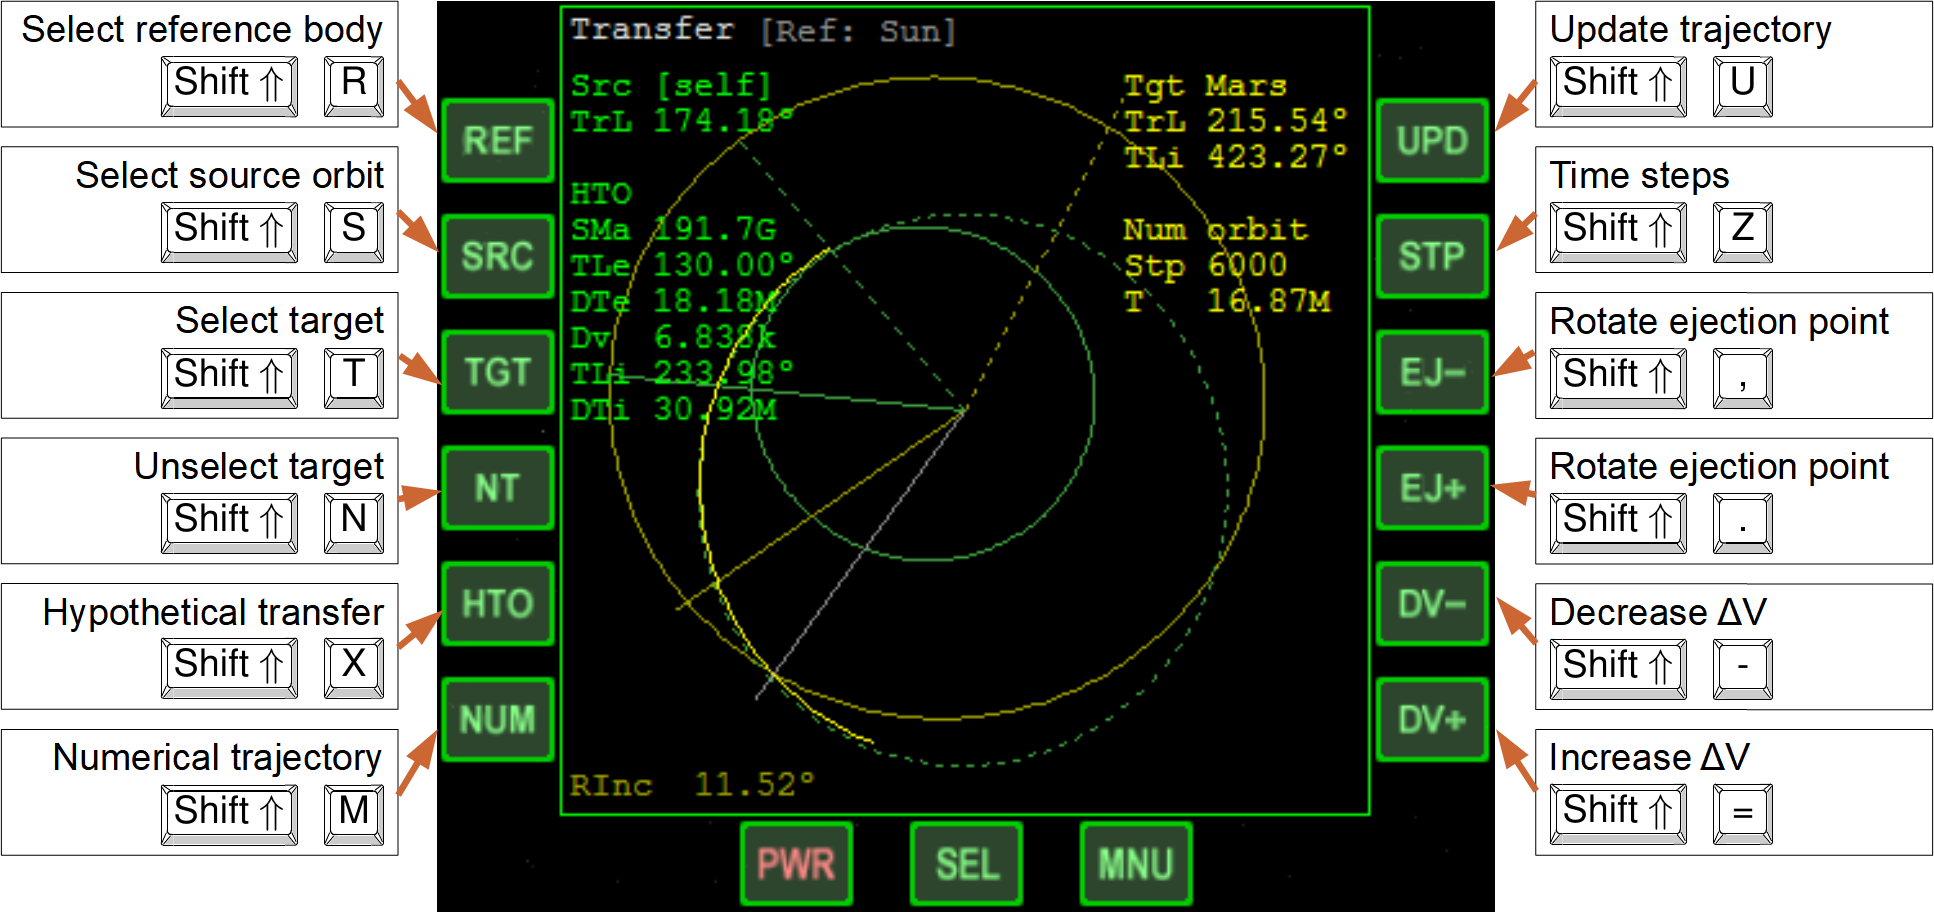
\includegraphics[width=0.99\hsize]{transfer_input_1.png}
\end{figure}

\begin{figure}[H]
  \centering
  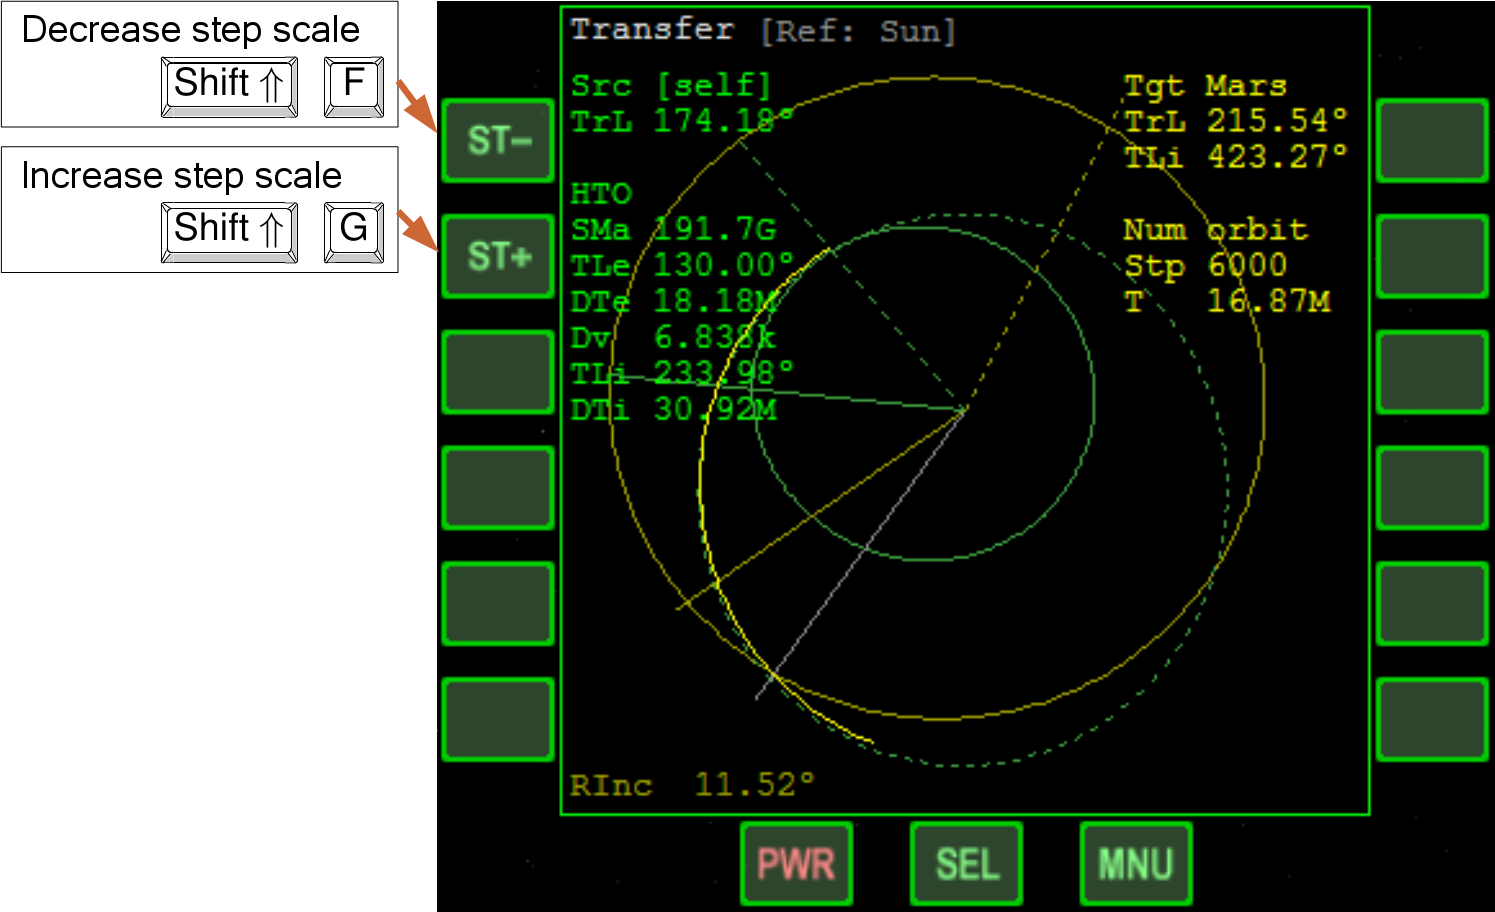
\includegraphics[width=0.75\hsize]{transfer_input_2.png}
\end{figure}

\noindent
\textbf{MFD display components:}

\begin{figure}[H]
  \centering
  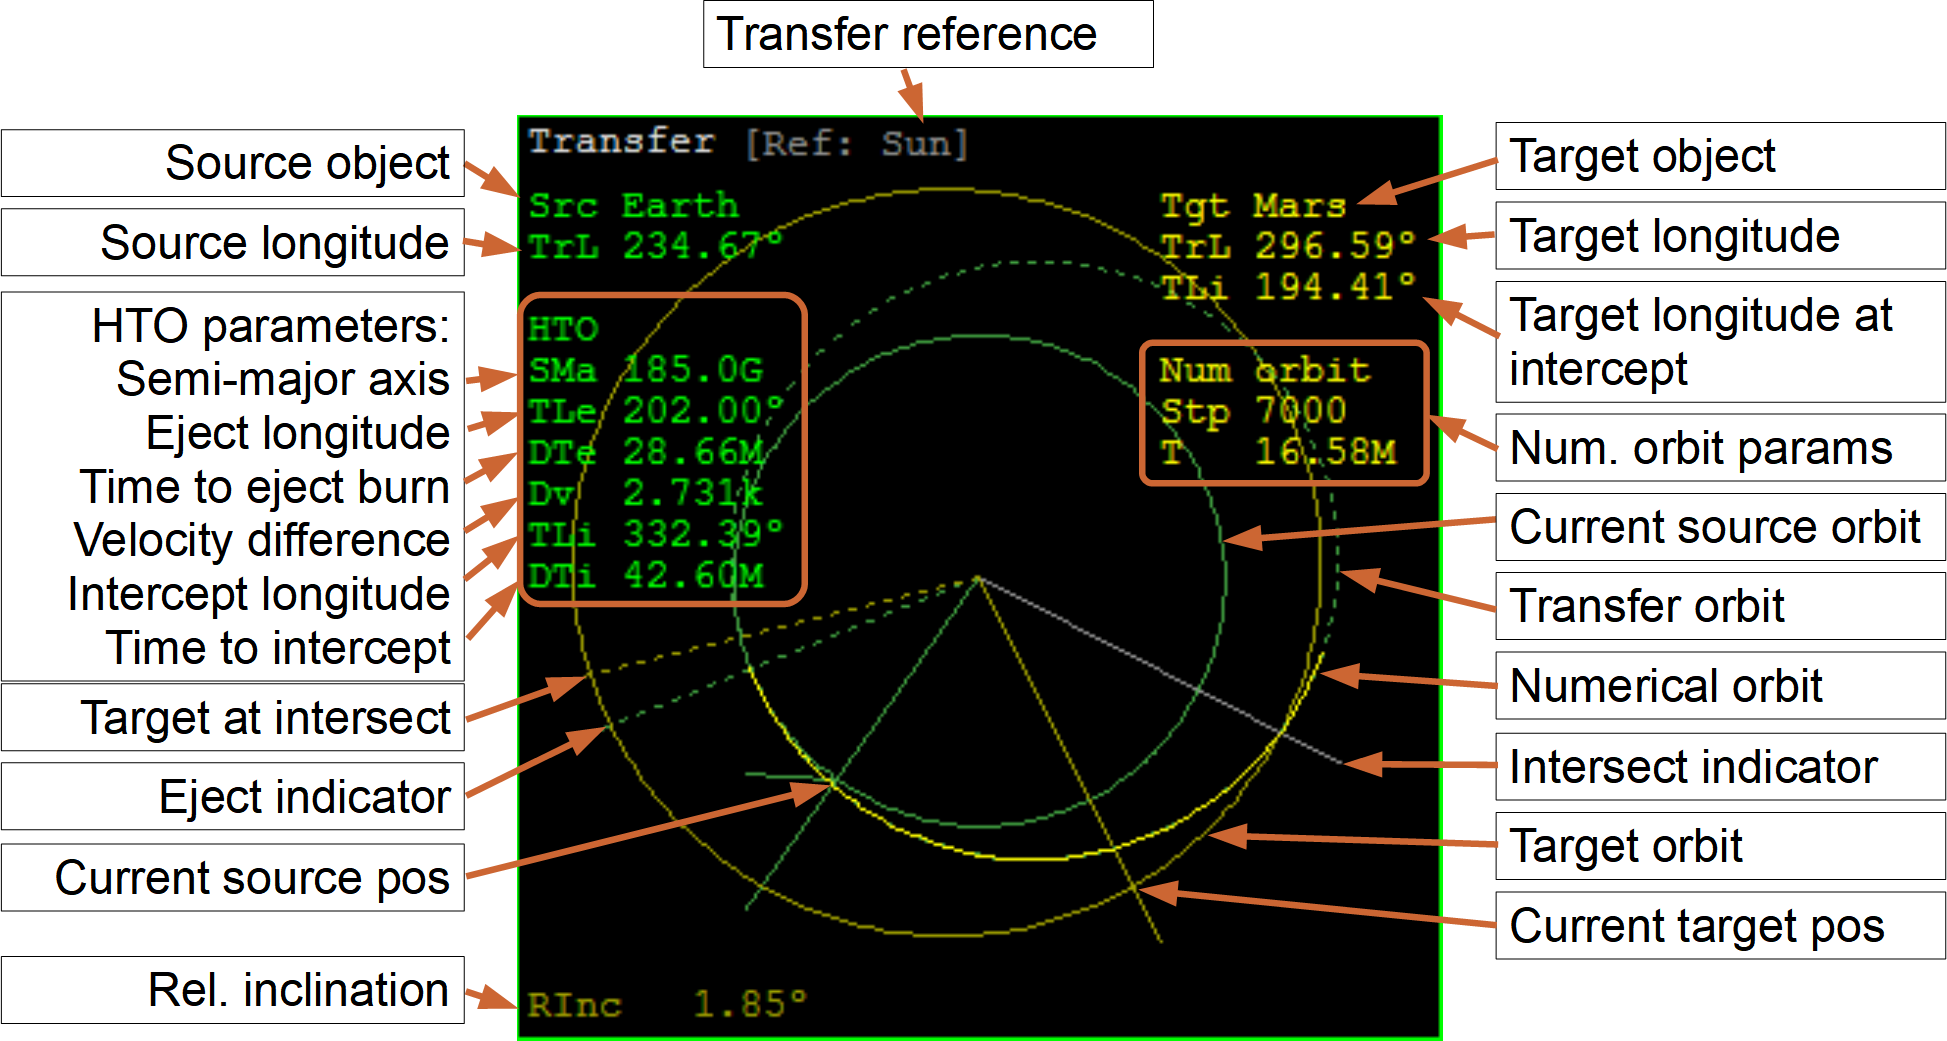
\includegraphics[width=0.99\hsize]{transfer_layout.png}
\end{figure}

\noindent
The Transfer MFD looks similar to the Orbit MFD: it displays a \textit{source} and \textit{target} orbit, relative to an \textit{orbit reference} body. The source orbit is usually your ship's current orbit, although sometimes a different source is more appropriate (see below). The Transfer MFD mode only works correctly for in-plane operation (i.e. assumes matching source and target orbital planes), although this condition usually can not be precisely satisfied for interplanetary transfers.\\
\\
\textbf{Source orbit selection}\\
The source orbit is the orbit from which to eject into the transfer orbit. Usually the source orbit will be the ship's current orbit. In certain situations however it is better to use a different source. Consider for example an interplanetary transfer from Earth to Mars, using the Sun as reference. Since the ship's primary gravitational source will be Earth rather than the Sun, its orbit with respect to the Sun will be strongly distorted by the Earth's gravity. In this case it is better to directly use Earth as the source object.\\
Whenever the source is a body other than the ship, a small direction indicator is displayed at the current source position which shows the ship's position relative to the source. This helps with timing the ejection burn. For example, to make use of the ship's orbital velocity around the source body, the ejection burn should take place when the direction indicator points away from the sun (assuming a prograde orbit).\\
\\
\textbf{Hypothetical transfer orbit}\\
To plan the transfer, a hypothetical transfer orbit (HTO) can be plotted given an ejection time and velocity difference (Dv), which allows to set up "what if" scenarios, before changing the actual orbit. The HTO display is toggled on/off with \Shift\keystroke{X}. It is calculated assuming that somewhere along the current source orbit a prograde or retrograde orbit ejection burn occurs. The HTO has two parameters: the longitude at which the ejection burn takes place (adjusted with \Shift \keystroke{,}/\keystroke{.}), and the velocity change during the burn (adjusted with \Shift \keystroke{-}/\keystroke{=}). The HTO is displayed as a dashed green curve. The position of the ejection burn is indicated by a dashed green radius vector.\\
A number of parameters is shown when the HTO is active:
\begin{itemize}
\item \textbf{SMa:} semi-major axis of the transfer orbit
\item \textbf{TLe:} True longitude of the orbit ejection point
\item \textbf{Dv:} Velocity difference from ejection burn
\item \textbf{TLi:} True longitude of intercept point with target orbit (if applicable)
\item \textbf{DTi:} Time to intercept with target orbit [s] (if applicable)
\end{itemize}

\noindent
\textbf{Intercept indicator}\\
If the source orbit (or, if shown, the HTO) intersects the target orbit, the intersect point is marked by a grey line, and the intersect longitude is displayed (TLi). The position of the target at the time when the ship reaches the intersect point is marked by a dashed yellow line. To plan an encounter with the target body, the objective is to adjust the HTO so that the grey and dashed yellow lines coincide (ship and target arrive at the intersect point simultaneously) by adjusting the ejection time and $\Delta$v.\\
\\
\textbf{Hohmann transfer orbit}\\
A transfer orbit which just touches the target orbit, and where ejection and intersect longitudes are 180° apart, is called a Hohmann minimum energy transfer orbit, because it minimises the amount of fuel used during the orbit ejection and insertion burns. Transfer orbits with larger major axis require more fuel, but are faster than Hohmann orbits.\\
\\
\textbf{Ejection burn}\\
Once the HTO has been set up, the ejection burn takes place when the ejection longitude is reached (when the solid and dashed green lines coincide). The ejection burn is prograde (or retrograde) given the orbit w.r.t. the current orbit reference. As the burn takes place, the current orbit (solid green line) will approach the HTO. The burn is terminated when the orbit coincides with the HTO and Dv has reached zero. After ejection the HTO should be turned off so that the intercept parameters are displayed for the actual transfer orbit.\\
\\
\textbf{Numerical multi-body trajectory calculation}\\
The source, target and transfer orbits discussed above are analytic 2-body solutions. The Transfer MFD however also supports a numerical trajectory calculation to account for the effect of multiple gravitational sources. The display of the numerical trajectory is toggled with \Shift\keystroke{M}. The trajectory is displayed as a solid bright yellow line. The calculation is performed in discrete time steps, starting from the current source position, or (if active) from the HTO ejection point. Since the calculation of the trajectory can be time-consuming, it is not automatically updated, but can be refreshed with \Shift\keystroke{U}. The interval between time steps is automatically adjusted to provide consistent accuracy. The number of time steps, and the total time interval covered by the trajectory segment, can be selected with \Shift\keystroke{Z}. The number of time steps and the total time interval, are displayed under \textit{Num orbit} in the MFD.\\
\\
\textbf{Interplanetary transfers}\\
Using the Transfer MFD for Earth to Moon orbits should be straightforward. For interplanetary transfers, e.g. Earth to Mars, a few caveats apply:
\begin{itemize}
\item For interplanetary transfers, the reference should be the Sun, and the source body should be the planet currently being orbited. This is because the ship's orbit relative to the Sun is significantly distorted by the planet.
\item The ship should be in an orbit with zero inclination against the ecliptic before ejection. The relative inclination between source and target orbits cannot be adjusted - it is simply given by the relative inclinations between the planets' orbits.
\item The ejection burn should take place with the Sun in opposition (on the planet's 'dark' side) so that the ship's orbital velocity is added to the planetary velocity. This is the case when the source $\rightarrow$ ship direction indicator is pointing away from the Sun.
\item Immediately before the ejection burn, switch the source orbit to your ship, so that Dv can be estimated.
\end{itemize}



\subsection{TransX}
\label{ssec:mfd_transx}
% TODO transx

\end{document}
